%\documentclass[10pt,preprint]{aastex}  % for e-submission to ApJ
%\documentclass[12pt,preprint2]{aastex}  % for e-submission to ApJ - two column
\documentclass[onecolumn,iop]{emulateapj}  % this makes everything look like ApJ

\usepackage{graphicx, natbib, color, bm, hyperref, breakurl}

%%%% PUT NEW COMMANDS AND DEFINITIONS HERE %%%%
%%%% PUT NEW COMMANDS AND DEFINITIONS HERE %%%%

\newcommand{\Lmax}{\ell_{\rm max}}
\newcommand{\enzo}{{\small Enzo}}
\newcommand{\moray}{{\small Enzo+Moray}}
\newcommand{\zeus}{{\small ZEUS}}
\newcommand{\Lbox}{L_{\rm box}}
\newcommand{\Nroot}{N_{\rm root}}
\newcommand{\K}{\,\rm K}

%dcc color commands
\newcommand{\gtt}[1]{\textcolor{green}{{\tt#1}}}
\newcommand{\red}[1]{\textcolor{red}{#1}}
\newcommand{\blue}[1]{\textcolor{blue}{#1}}
\newcommand{\dcc}[1]{\textcolor{blue}{{\emph{#1}}}}

%mqk commands
\newcommand{\mqk}[1]{\textcolor{red}{mqk: #1}}
\renewcommand{\div}{\bm{\nabla} \cdot}
\newcommand{\grad}{\bm{\nabla}}
\newcommand{\curl}{\bm{\nabla} \times}

%%%% use this if you want \paragraph{} sections to be numbered.
%% \setcounter{secnumdepth}{5}

%dcc misc defs.
\def\grid{{\tt grid}}

\def\etal{{\sl et al.}}
\def\kms{{\rm km/s}}
\def\Ms{{\rm M_\odot}}
\def\nd#1{n_{ \rm #1}}
\def\k#1 {k_{{\rm #1}}}
\def\HH{H$_2$}
\def\HHp{H$_2^+$}
\def\Hp{H$^+$}
\def\Hm{H$^-$}
\def\Hep{He$^+$}
\def\Hepp{He$^{++}$}
\def\Dp{D$^+$}
\def\mHH{H_2}
\def\mH2p{H_2^+}
\def\mHp{H^+}
\def\mHm{H^-}
\def\mHep{He^+}
\def\mHepp{He^{++}}

%GB commands (overview section):
\newcommand{\myvec}[1]{\mathbf{#1}}
%\newcommand{\myvec}[1]{\vec{#1}}  %uncomment for traditional vectors
\newcommand{\rhop}{\rho^\prime}
\newcommand{\vecvp}{\myvec{v}^\prime}
\newcommand{\vecv}{\myvec{v}}
\newcommand{\vecB}{\myvec{B}}
\newcommand{\vecx}{\myvec{x}}
\newcommand{\Ep}{E^\prime}
\newcommand{\ep}{e^\prime}
\newcommand{\phip}{\phi^\prime}
\newcommand{\pp}{p^\prime}
\newcommand{\vecr}{\myvec{r}}
\newcommand{\rhob}{\rho}
\newcommand{\vecvb}{\vecv}
\newcommand{\Mach}{\mathcal{M}}
\newcommand{\fcond}{\myvec{F}_{\rm cond}}
\newcommand{\minmod}[2]{{\rm minmod} \left({#1},{#2} \right) }

%JHW commands
\newcommand{\cubecm}{\ifmmode{{\rm cm^{-3}}}\else{cm$^{-3}$}\fi}
\newcommand\unit[1]{\; \textrm{#1}}
\newcommand{\mh}{m_{\rm H}}

%SWS commands
\newcommand\abs[1]{\left|#1\right|}



%%%%%%%%%%%%%%%%%%%%%%%%%%%%%%%%%%%%%%%%%%%%%

% Paper Outline  (last updated May 17, 2013)
%
% 1.  Introduction
% 2.  Physical equations and overview of numerical methodology
%   2.1 Physical equations
%   2.2 Overview of numerical methods
% 3.  The structured AMR method
% 4.  Fluid methods
%   4.1 PPM
%   4.2 MUSCL
%   4.3 MHD-CT
%   4.4 ZEUS 
% 5.  Gravity and N-body
%   5.1 Gravity
%   5.2 N-body dynamics
% 6. Microphysics
%   6.1  Chemistry
%   6.2  Radiative Cooling and heating
% 7. Radiation
%   7.1 Radiation: Homogeneous
%   7.2 Radiation: ray-tracing
%   7.3 Radiation: FLD
% 8. Other physics
%   8.1 Thermal conduction
%   8.2 Star formation & Feedback
% 9. Timestepping
% 10.  Analysis
% 11. Code tests
%   11.1 Verifying and Validating the Enzo code
%   11.2 Representative test problems
% 12. Parallelism 
%   12.1 Parallel strategy 
%   12.2 Parallel performance 
% 13. Code development methodology
% 14. Conclusions
%
%%%%%%%%%%%%%%%%%%%%%%%%%%%%%%%%%%%%%%%%%%%%%

\citestyle{aa}  % correct formatting for ApJ style files

\begin{document}

\title{Phd: Phython Hydro-Dynamics Code for Astrophysics}
\author{Ricardo Fernandez\altaffilmark{1}}
\author{Greg L. Bryan\altaffilmark{1,2}}

\altaffiltext{1}{Columbia University, Department of Astronomy, New York, NY, 10025, USA}
\altaffiltext{2}{Center for Computational Astrophysics, Flatiron Institute, 162 Fifth Avenue, New York, NY 10010}

\begin{abstract}
This paper describes the open-source code \enzo, which uses
block-structured adaptive mesh refinement to provide high spatial and
temporal resolution for modeling astrophysical fluid flows.
\end{abstract}

\keywords{methods: numerical --- hydrodynamics}

\maketitle

%% Section: introduction
\section{Introduction}
\label{sec.intro}

The use of numerical simulations for modeling astrophysical compressible 
gas have steadily grown through the rise of computing power and decrease
in price of hardware. Astrophysical problems poses its unique set of challenges
manifesting throught its high spatial and temporal dynamic ranges. Progress
has been made over the years by the development of algorithms that leverage
computing resources to the problem at hand. The two most notable numerical methods 
are Langrangian and Eulerian schemes. A popular example of Langrangian scheme
is the smoothed particle hydrodyanmics developed by ... 

In this scheme
talk  about sph strengths and weakness

talk about eulerian

talk

For example adaptive mesh refinement
allows for dynamic addition of computing grids. This feature allows computing
resources to adaptively  

\subsection{Motivation for ALE}
\label{sec.motivation_ale}

Due to the high spatial and temporal dynamical ranges involved,

\subsection{Motivation for Python}
\label{sec.motivation_python}

Due to the high spatial and temporal dynamical ranges involved,

\subsection{Design Philosophy}
\label{sec.design_philosophy}

Due to the high spatial and temporal dynamical ranges involved,


% Section:  Overview
\section{Code Design}
In the following section we go over the design and rationale of our choices
for the development of the code. In several instances we will describe 
methods that we believe are the most important and give examples of 
implementation and modification.

\subsection{Overall Class Design Considerations}
\subsubsection{Field Registration}
Form our past experience, we have found one of the challenging problems in maintaining codes
is that of adding new fields. There are many reasons why to add new fields, for example,
an implementation of new physics (MHD, radiation, chemistry etc.) or adding a passive scalar
to track some portion of the fluid or modification of an existing algorithm that needs an auxiliary
field which has not been stored. In any case, the addition of a new field can be challenging
if the computation has been hard coded or the data structures, for example C structs, do not
allow the addition of new fields. For this reason, we early on adopted a data structure
that allows registration of fields (see Section~\ref{sec.carraycontainer}). In this manner
fields can be easily added in the future.

From these considerations we will see a common thread with our classes, most have a method
for field registration or addition:
\begin{itemize}
	\item \lstinline{register_fields()} add fields to the simulation.
    \item \lstinline{add_fields()} add fields to self by inspecting current simulation fields.
\end{itemize}
For registration, the class usually inspects the particle data structure and creates fields
necessary for the simulation. As an example, gravity registers the acceleration to the particles
in the proper dimension. In this manner, we don't have unnecessary fields during the simulation
(3D fields for 2D runs). Likewise, for addition of fields the class usually inspects the
particle data and proceeds to register the proper fields internally. For example, gravity 
registers internally tree moment fields with the proper dimension.

Since any number of fields can be registered, we have also allowed the ability to group
fields by names. This has been extensively used to group collection of fields like
primitive and conservative fields. This has allowed to easily retrieve collection of fields
that are related and can be computed as a collection.

\subsubsection{Class Dependencies}
Another source for future problems is when an algorithm depends on another. For example
our gravity tree solver depends on our load balance implementation. If the algorithms
are designed concurrently, then proper consideration is taken on how they will
interact with one another. However, because of developments of new algorithms or experimentation, 
classes will eventually need to interact with others that where not originally designed for. In these
situations common options are to re-factor the algorithm or even rewrite the algorithm itself. Both 
methods can become cumbersome as the code develops and matures and changing one portion of the code 
may create a cascade of other changes.

In our case we decided to write our classes as encapsulated computations. This means we have
tried to segregate computations as independent tasks and interactions between classes are 
defined through their api. For the most part, each computation has a base class (i.e 
\lstinline{ReconstructionBase}, \lstinline{RiemannBase}, \lstinline{InetgrateBase} etc.) that
defines the methods it can perform. Moreover, the base class only serves as a template and
returns a warning if accessed. Thus, each implementation inherits the base class and defines
the actual computation. Further if a method depends another class it has to be written in
the confines of the api. Therefore, our algorithms are designed in confirm to an api
and any development of a future class will have to abide by it.

\subsection{Particle Data Structures}
\subsubsection{Carray}
In choosing the underlying data structure several considerations where taken. First the
data had to be accessible in python and in C. Second the data structure had to
accommodate several data types. For this reason we choose a data structure that mimics
numpy arrays, in the sense that raw data is allocated in C and interface exist that
manipulates the data in either C or python. With this approach a decision had to be
made in the form of the raw data. Two choices where considered, either the data would
be held in structs or arrays. The benefit of structs would allow subfields of the data
be compact and allow easy implementations of passing and receiving data from other
processors in parallel runs. Further numpy has an interface, that treats
arrays of structs as record numpy arrays. However, this form was abandoned early on
as the sub-fields would have to be hard coded and would not allow the creation of
dynamic fields at run time. With this consideration, the raw data was chosen to be
C arrays. 

The exact implementation was taken from pysph code. The class is called Carray and
can be initialized in Python or Cython. The interface closely resembles the list
class of C++, in allowing indexing and memory management. Further, Carrays can return
a numpy array, allowing the user to use all numpy functional (i.e. slicing and fancy indexing). 
Below is a simple example using a Carray.
\begin{lstlisting}
import phd

x = phd.DoubleArray(10)
for i range(len(x)):
	x[i] = i**2
    
x.append(3.21)
x.resize(5)

xnp = x.get_npy_array()
xnp[:] = np.arange(x.length)
\end{lstlisting}
In this example a Carray is created with 10 doubles, then assigned values by indexing. Notice
that the length of the Carray can be found either by the len function or the length
attribute. The Carray then has a value appended to it followed by resizing the Carray to a length
of 5. Finally, the get npy array is called returning a numpy array which allows the use of slicing.

\subsubsection{CarrayContainer}
\label{sec.carraycontainer}
The use of Carrays allow to easily manipulate arrays of certain type of data. However, there are
many circumstances for the need of a collection of Carrays. For example the x, y, and z position
of a particle or the center of mass and moments of a node in the gravitational tree. Therefore,
another data structure has been implemented to facilitate the use of collection of Carrays. The data
structure is called a CarrayContainer and like the Carray it has many methods to manipulate the
underlying data. The CarrayContainer in some aspects mimics a python dictionary in the sense
that each carray can be retrieved by a string key.
\begin{lstlisting}
import phd
import numpy as np

carrys = {"x": "double", "y", "double"}

ca_con = phd.CarrayContainer(10, carrays)
size = ca_con.get_carray_size()
ca_con["x"][:] = np.random.rand(size)
ca_con["y"][:] = np.random.rand(size)

ca_con2 = phd.CarrayContainer(5, carrays)
size = ca_con.get_carray_size()
ca_con["x"][:] = np.random.rand(size)
ca_con["y"][:] = np.random.rand(size)

ca_con.append(ca_con2)
ca_con.remove(np.array([1, 3, 9])
\end{lstlisting}
Most of the routines of Carrays have been extended to CarrayConatiner to operate on
all Carrays in the Container. Further the container has routines to subset, remove, paste
and add values to certain elements.

\subsection{Simulation Class}
The \lstinline{Simulation} class is the main driver for advancing the solution in time
and coordinating outputs to disk and terminal. The two most important methods of this
class are listed below
\begin{itemize}
    \item \lstinline{solve()}: advance \lstinline{IntegrateBase} to its final state while
        outputting all necessary information. 
    \item \lstinline{compute_time_step()}: aggregate all time steps and enforce the smallest.
\end{itemize}
From its inception, the class was designed to be independent of the solvers. This was 
accomplished by distinguishing state computation and state advancing methods. For example,
\lstinline{IntegrateBase} can only perform a computation at a given temporal state 
(see Section~\ref{sec.integrator} for details) while \lstinline{Simulation} can
dictate when and the number of computations. Thus, \lstinline{Simulation} controls the
time advancement independently of the equations being solved. As of writing three integrators
exist, however, adding a new integrator is relatively straightforward.

During the course of a simulation the class is responsible to schedule outputs and
determined if the simulation has completed. Simulation outputs and termination are 
designated by the \lstinline{SimulationOutputerBase} and \lstinline{SimulationFinisherBase} 
classes respectively (see Section~\ref{sec.outputters} for details). At the end of every time
step the class calls \lstinline{compute_time_step()} to modify the current time step and
output any necessary data by cycling through all outputters. Likewise, at the beginning of
the time step the class cycles through all \lstinline{SimulationFinisherBase} classes 
in search for a termination signal.

Lastly, the simulation class also controls logging information (see Section~\ref{sec.logging}
for details). 
Log information is currently printed to the terminal and saved to a log file. The simulation class 
allows the ability to pick how much information should be printed and saved. In parallel runs, the 
root processor takes responsibility for writing to the log file and displaying to terminal.

\subsubsection{Serialization of classes and parameters}

\subsection{Mesh Class}
\subsubsection{Tessellation}
\subsubsection{Grid Motion}
\subsubsection{Flux Update}

\subsection{Integrator Class}
\label{sec.integrator}
1. current implementations, hard code solver
2. need to allow the ability to quickly create solver for different
   physics or algorithm.
3. Our implementation allows for this
4. Since all our computation are core blocks we can build a solver
   by selecting the calls
6. we currently have three implementations 

The implementation of the equaitons to be solved are performd throught
the \lstinline{IntegrateBase} class. This class is responsible to perform
the nesscary actions to progress the equations to one time step. The
integrator uses the other classes as building blocks. Currently we 
have implemented the static and moving mesh muscle hancock scheme
and a leap frog integrator. The idea is to separate the order of computation
from the simulation and core computation. In this way any solver can
quickly built by inheriting the solver. 

The api is listed below:
\begin{itemize}
    \item \lstinline{before_loop()}
    \item \lstinline{compute_time_step()}
    \item \lstinline{evolve_time_step()}
    \item \lstinline{after_loop()}
\end{itemize}


\begin{lstlisting}
def evolve_timestep(self):
    """Solve the compressible gas equations."""

    phdLogger.info("StaticMeshMUSCLHancock: Starting integration")

    # build left/right states at each face in the mesh
    self.reconstruction.compute_gradients(self.particles, self.mesh,
            self.domain_manager)
    self.reconstruction.compute_states(self.particles, self.mesh,
            self.equation_state.get_gamma(), self.domain_manager, 0.5*self.dt,
            self.riemann.boost)
    self.compute_source("primitive")

    # solve riemann problem, generate flux
    self.riemann.compute_fluxes(self.particles, self.mesh, self.reconstruction,
            self.equation_state)

    # update conservative from fluxes
    self.mesh.update_from_fluxes(self.particles, self.riemann, self.dt)
    self.compute_source("flux")
    self.compute_source("compute")

    self.compute_source("conservative")
    self.domain_manager.update_ghost_fields(self.particles,
            self.particles.carray_named_groups["conservative"],
            True)

    # convert updated conservative to primitive
    self.equation_state.primitive_from_conservative(self.particles)
    self.iteration += 1; self.time += self.dt
\end{lstlisting}

\begin{lstlisting}
def evolve_timestep(self):
    """Evolve the simulation for one time step."""

    # kick
    for ax in self.axis:
        self.particles["velocity-"+ax][:] += 0.5*self.dt*self.particles["acceleration-"+ax][:]

    # drift
    for ax in self.axis:
        self.particles["position-"+ax][:] += self.dt*self.particles["velocity-"+ax][:]

    if phd._in_parallel:
        self.load_balance.decomposition(self.particles)

    # compute new acceleration
    self.gravity_tree.build_tree(self.particles)
    self.gravity_tree.walk(self.particles)

    # kick
    for ax in self.axis:
        self.particles["velocity-"+ax][:] += 0.5*self.dt*self.particles["acceleration-"+ax][:]

    self.iteration += 1; self.time += self.dt
\end{lstlisting}

\subsection{Hydro Class}
\subsubsection{Reconstruction}
\subsubsection{Riemann Solver}

\subsection{General Source Terms}
The inclusion of source terms has been implemented through a general source
\lstinline{SourceTermBase} with methods listed below:
\begin{itemize}
    \item \lstinline{apply_primitve()}: modify primitive variables.
    \item \lstinline{apply_conservative()}: modify consevative variables.
    \item \lstinline{apply_flux()}: modify flux terms.
    \item \lstinline{compute_source()}: calculate soure components.
    \item \lstinline{compute_time_step()}: calculate time step from source term.
\end{itemize}
This formulation was chosen after some considerable experimentation. One of the
earlier attempts was a registration process. In this scenario a source term
would link any computation to class method. This information was stored
in a dictionary inside \lstinline{Simulation} and at runtime each class method
was over written using Pythons decorator shcheme. Although, this scheme makes
use of more advnace programming methods we found that this implementation was
not easy to discern. Moreover we found that this method left to much ambiguity
to the source terms, allowing . Instead we
found this current implementation to be more understanble and easier to
generalize.

The api listed above are the mandatory methods to be defined for any source
term. In general, we write an interface for each given source term. In this
way if the integrator changes only the api has to be updated leaving
the core of the source term unaltered. This also allows to easily implement
third party libraries as source terms, chemsitry or radiation for example.
Once the methods have been defined the class is registered to 
\lstinline{Simulation} class and will be invoked at the appropriate parts
during the computation.

\subsubsection{Gravity}
For a more concrete example of how to include a source term we highlight the
pieces used to include self gravity. Our self gravity is a tree based implemetation
named \lstinline{GravityTree}. Its main routine is \lstinline{walk()} which is the
calculation of gravitational accelerations from the current position of the particles.
To include this as a source term we created a new class called \lstinline{SelfGravity}
which inherits \lstinline{SourceTermBase}. As disscussed in section, gravity alters
the momentum and primitive values.
\begin{lstlisting}
...
cdef class SelfGravity(MUSCLHancockSourceTerm):
    ...
    cpdef apply_primitive(self, object integrator):
        # loop over each face in the mesh 
        for m in range(integrator.mesh.faces.get_carray_size()):
            ....
            # add gravity to velocity
            for k in range(dim):
                vl[k][m] += 0.5*dt*a[k][i]
                vr[k][m] += 0.5*dt*a[k][j]

        # add gravity acceleration from particle
        for i in range(integrator.particles.get_carray_size()):
            ...
                for k in range(dim):
                    # update momentum
                    e.data[i] += 0.5*dt*mv[k][i]*a[k][i]

                    # update energy 
                    mv[k][i] += 0.5*dt*mass.data[i]*a[k][i]

    cpdef apply_conservative(self, object integrator):
        ...
        # add gravity acceleration from particle
        for i in range(integrator.particles.get_carray_size()):
            ...
                for k in range(dim):
                    # update momentum
                    mv[k][i] += 0.5*dt*mass.data[i]*a[k][i]

                    # update energy 
                    e.data[i] += 0.5*dt*mv[k][i]*a[k][i]
\end{lstlisting}

\subsection{Readers/Writers}
\subsubsection{HDF5}

\subsection{Outputters and Finishers}
\label{sec.outputters}

\subsubsection{Design API}
The code has been desinged to handle arbritary signals for outputing data
and completion of the simulation. This has been achieved by introducing the
\lstinline{SimulationOutputerBase} class for output and
\lstinline{SimulationFinisherBase} class for completion.

At the end of every
time step (\lstinline{SimulationOutputerBase} includes the beginning and ending
of the simulation) a call to all registered outputers and finishers is
performed. In each call the class has complete control of the integrator. Thus
the classes can inspect the time, time step, iteration, particle data, flux data,
reconstruciton data etc. This allows for a general conditions instead of hard
coded ones. Further this opens the door to allow conditions

the options are plentiful and we hope to make large of use in the next
revision of the code.

In the case of \lstinline{SimulationOutputerBase} a writer is registered with it.

\subsubsection{Examples}
In this section we show, some what trivial but highlights the main points, an example of
how to create an outputter and finisher. For our example, we use the sedov problem from 
section cite. We are interested to output all time steps once the shock has reached
a density $\rho=2$ and remains less than $\rho=3$. Of course in this situation one may
use the analytical solution to extraplote when such values would occur. However that
assumes the shock track exactly. In our scenario we let the simulation do the work
for us.

First we begin by defining an outputter with the objective to start outputing
all data once the density value of $\rho=2$ has been reached (see code excerpt). This
is accomplished by inherting \lstinline{SimulationOutputerBase} and modifying
\lstinline{check_for_output} and \lstinline{modify_timestep}. For over writing
\lstinline{check_for_output}, we check is the the outputter is the main loop state
and if the max density is greated than \lstinline{density_min}. Moreover, there
is no need to change the time step, therefore, it is left unaltered.


\begin{lstlisting}
...
class OutputSedovDensity(SimulationOutputerBase):
    def __init__(self, density_min, base_name="density_output",
                 counter=0, pad=4, **kwargs):
        super(OutputSedovDensity, self).__init__(base_name, counter, pad, **kwargs)
        self.density_min = density_min 

    def check_for_output(self, simulation):
        """Return True to signal the simulation has reached
        sedov interval to ouput data."""
        integrator = simulation.integrator
        state = simulation._state == SimulationTAGS.MAIN_LOOP
        output_sedov = integrator.particles["density"].max() >= self.density_min:

        if state and output_sedov:
            return True
        return False

    def modify_timestep(self, simulation):
        """Return consistent time step."""
        # not modifying
        return simulation.integrator.dt

\end{lstlisting}
At this point our data will be outputted untill the simulation is finished. To
create a finisher at the moment when density has reached $\rho_{\mathrm{max}}$
we create a new class \lstinline{SedovDensityFinisher}. This class inherits
\lstinline{SimulationFinisherBase} and one needs to define the \lstinline{finished}
method. In our case we need only to compare our max density values with
$\rho_{\mathrm{max}}$.
\begin{lstlisting}
...
class SedovDensityFinisher(SimulationFinisherBase):
    def __init__(self, density_max, **kwargs):
        self.density_max = density_max

    def finished(self, simulation):
        """Return True to signal the simulation is finished
        if reached max iteration number.
        """
        if simulation.integrator.particles["density"].max() >= self.density_max:
            return True
        else:
            return False

\end{lstlisting}

Although are example was simplistic, we hope that it shows the flexibility and power
what the outputters and finishers may achieve.  

\subsection{Load Balance}

\subsection{Equation of State}
Our equation state is implemented through \lstinline{EquationStateBase}. We
decided 
\begin{itemize}
    \item \lstinline{conservative_from_primitive()}: modify primitive variables.
    \item \lstinline{primitive_from_conservative()}: modify conservative variables.
    \item \lstinline{sound_speed()}: modify flux terms.
    \item \lstinline{get_gamma()}: calculate source components.
\end{itemize}


\subsection{Domain Manager}
Our \lstinline{DomainManager} class is designed to handle information associated with
the domains of the simulation. We consider a domain to be the spatial region where the computation
is performed. In serial, this is the entire spatial region of the simulation.
In parallel, this is the spatial region associated with each processor. 
In this way, for the most part, our domains are isolated computations and when
data is needed from neighboring domains they are requested through the \lstinline{DomainManager}.

The \lstinline{DomainManager} was initially designed to contain the limits and dimension of
the problem. As development continued it became natural that the \lstinline{DomainManager} would
encompass the boundary condition, ghost particle information, and exchange of data across boundaries.
At its current state, the \lstinline{DomainManager} only supports communication of ghost particle data
and does not support the general forms of data communication
(i.e reduction, gathers, broadcast etc). We plan in the next revision to implement an api that
performs these task. In doing so, we would remove strict dependence on MPI functions and only
work through the \lstinline{DomainManager}.

\subsubsection{Internal Boundary Particle Sharing}
In parallel, particles are decomposed into a disjoint set of spatial domains
with each domain mapped to a unique processor. The construction
of the global Voronoi mesh is then delegated to the construction of a disjoint set
of local Voronoi meshes. For the set of local constructions to be consistent
with the global mesh, the appropriate boundary particles must be 
communicated across domains.

Interior ghost particles, are particles formed from neighboring domains and are used to
connect local meshes together. Their creation is handled by the \lstinline{DomainManager}
through the \lstinline{create_interior_ghost_particles()} method. This method
creates interior ghost particles by inspecting the search radius of
each local particle. If a particles search radius overlaps with a processor
boundary then it is flagged and a corresponding ghost particle is created and exported to that processor.
The search method is made possible by the \lstinline{DomainManager}s ability to query
all domains through geometrical searches. Care is taken such that no duplicates are created through the 
whole process. After each particle is inspected, ghost particles are communicated and then the
mesh is allowed to updated itself. This procedure is repeated until particles are no longer flagged.

\subsubsection{Boundary Condition}
Similar to interior ghost particles, exterior ghost particles are used to
complete local meshes. However, exterior ghost particles are not from neighboring
domains but instead are created through a boundary condition. To allow for different
boundary condition we have created \lstinline{BoundaryConditionBase} that interacts
with \lstinline{DomainManager}. The api is listed below:
\begin{itemize}
	\item \lstinline{create_ghost_particle()} create ghost particle from flagged particle.
    \item \lstinline{migrate_particles()} for particles that have left the domain, apply
    appropriate boundary condition.
    \item \lstinline{update_gradients()} apply boundary condition to ghost particle gradients.
    \item \lstinline{update_fields()} apply boundary condition to ghost particle fields.
\end{itemize}
Through this api, any boundary condition may be implemented. The boundary condition does not have
to be uniform in each dimension. Mixed boundaries or even problem specific boundaries are allowed
in this framework. Furthermore, the api allows the boundary
condition to modify particle motion and field data. In this way, we have extracted all boundary
information from the \lstinline{DomainManager}.

Currently, we have two implementations of boundary conditions, reflective and periodic.
In the reflective case, the flagged particle is mirrored across each boundary edge of the
simulation. If an intersection occurs, a ghost particle is created with its normal velocity flipped.
In the serial case, the ghost particle is added directly to the particle data container. In parallel, the 
ghost particle is then further inspected for intersection of neighboring processors. The ghost particle
is then placed in a communication to be exported to each flagged processor. For the periodic case
the procedure is similar, with the exception that particle is periodically shifted
instead of being mirrored.

\subsubsection{Data Communication}
After the creation of ghost particles, in parallel simulations, supplemental data has to be communicated. 
For example, the center of mass may not be computed locally because its neighbors may not exist locally.
This is because our implementation of ghost particles only to guarantees all neighbors of local
particles. Certainly we could of opted to import all neighbors of ghost particles but instead we have 
decided to communicate that information instead. Thus, the \lstinline{DomianManager} records all information
associated with a ghost particle. This allows ghost particles to be easily updated with any data. These
operations are implemented through \lstinline{update_ghost_fields()} and 
\lstinline{update_ghost_gradients()}

\subsubsection{Particle Motion}
After a flux update, the particles are allowed to move. Depending on initial particle position and
velocity a particle may leave its processor or the simulation domain. In either case, the 
\lstinline{DomainManager} is responsible for the destintation of the particle.

When a particle leaves the simulation domain in serial or parallel the \lstinline{DomainManager}
flags that particle and then applies the boundary condition. For reflective boundaries the particle is not
allowed to leave and for periodic boundaries the particle is wrapped back into the domain. If the simulation
is in parallel the \lstinline{DomainManager} exports the particle to the correct processor and removes
it from the local particle container. If a particle leaves its processor patch the \lstinline{DomainManager}
will query all domains and find the correct domain for export.

\subsection{Logging}
\label{sec.logging}
Event logging during a simulation is performed through the python 
\texttt{logging}\footnote{\url{https://docs.python.org/2/library/logging.html}} library. The library has 
many capabilities but for our intentions we have focused on displaying and storing messages related to the
state of the simulation. To that end, we use one logger called \lstinline{phdLogger}. This 
logger can be imported to any file and used to log any information of interest.

For our purposes, the logger has four levels of logging. They are listed below:
\begin{itemize}
	\item debug: detailed information or diagnosing.
    \item info: working as expected.
    \item success: a successful completion. 
    \item warning: unexpected result that may lead to future problem.
\end{itemize}
The log levels have been listed in order of inclusion. Meaning if ``warning'' is chosen, then all messages
types are logged. However if ``info'' is chosen only messages of type ``debug" and ``info'' or logged.
At runtime the log level and file to store the messages can be specified through the 
\lstinline{Simulation} class.

As an example we show a simple usage of the logger below:
\begin{lstlisting}
import logging
phdLogger = logging.getLogger("phd")
...
phdLogger.info("Starting kinetic energy calculation")
kinetic_energy = particles["mass"]*(particles["velocity-x"]**2 + particles["velocity-y"]**2)

if kinetic_energy.sum() > 0:
	phdLogger.debug("Kinetic energy greater than zero")
\end{lstlisting}
In this example we import the logger and print out a messages related to the calculation of the
kinetic energy. It is important to note that this example is true if run in serial or parallel. The logger
has been modified such that logging information and storage is always handled by the root processor.


% We now describe each of the numerical methods in detail in their own
% sections

In this section, we describe the four solvers that we have implemented
for solving the fluid equations.  We describe the PPM method in
considerably more detail than the other methods in part because its
implementation in Enzo has not previously been described, but mostly
because it introduces many of the ideas and methods used for the
MUSCL-Dedner and MHDCT schemes (including expansion terms,
reconstruction, Riemann solvers, and dual energy formalism).

\subsection{Physical Equations}

\subsection{Tessellation}

\subsection{Fluid Update}
\subsubsection{Reconstruction}
\subsubsection{Riemann Solve}
\subsubsection{Flux Computation}
\subsubsection{Time Integration}

\subsection{Grid Motion}
\subsubsection{Regularization}

\subsection{External Boundary Conditions}

\subsection{Gravity}
\subsubsection{Tree}
\subsubsection{Particle Mesh}

\subsection{Chemistry and Cooling}

\subsection{Additional Physics}


% Section: code tests
\section{Tests}
\subsection{Unit Tests}

\subsection{Hydro Tests}
In this section we present a series of tests to help verify the integrity and stability
of the hydrodynamic algorithms used. For each test it is assumed that linear reconstruction,
mesh movement, motion correction, and HLLC algorithm was used unless stated otherwise. We
have found the HLLC, in most cases, to be as accurate as the Exact solver. In doing so, we have 
chosen the HLLC as our default solver as it is more accurate than the HLL and less computational 
intensive then the Exact solver. All scripts to generate the simulations and plots will be found
in the \textbf{test\_suite} directory.

\subsubsection{Linear Wave}
Sound waves provide the mechanism to transport disturbances through a fluid. An
elementary test problem is the ability maintain wave propagation of small
disturbances. Given a fluid in equilibrium with constant density $\rho_0$,
pressure $P_0$ and zero velocity $\mathbf{v}=0$ with perturbations of the form
\begin{equation}
	\begin{array}{rcl}
		\rho & = & \rho_0 + \delta\rho(x,t) \\
   		 P & = & P_0 + \delta p(x,t) \\
    	\mathbf{v} & = & \delta\mathbf{v}(x,t),
    \end{array}
\end{equation}
and maintaining terms to first order in the Euler equations produce the wave
equation for each variable with sound speed equal to the fluid's sound speed 
$c_s$. Thus, setting a small disturbance 
will propagate with a finite velocity maintaining its form as along as the initial
disturbances are relatively small.

We set up a 2d box of unit length with constant $\rho_0=1.0$, $P_0=3/5$, $\mathbf{v}=0$,
and $\gamma=5/3$ with periodic boundary conditions. A sinusoidal wave in the $x$ direction of 
the form $\delta\rho(x,t) = A\mathrm{sin}(kx + wt)$ with $k=w=2\pi$ and $A=10^{-6}$ is added at 
time $t=0$. The remaining disturbances can be specified through $\delta\rho$ by the following
\begin{equation}
	\begin{array}{rcl}
        \delta \mathbf{v}(x,0) & = & \left(\frac{w}{k}\right)\delta
        	\rho(x,0)/\rho_0\mathbf{\hat{x}}\\
        \delta P(x,0) & = & \left(\frac{w}{k}\right)^2\delta\rho(x,0).
    \end{array}
\end{equation}
The values chosen produce waves traveling rightward with a velocity of 1. The simulation is
evolved for 1 unit of time such that the waves return to its' initial position at time $t=0$. 
Moreover, we study the convergence behavior by comparing the final state of the density to 
the initial density by computing the $L1$ norm,
\begin{equation}
	L1 = \frac{1}{N^2}\sum_i \left| \rho_i - \rho(x_i) \right|,
\end{equation}
where $\rho_i$ is final density at position $x_i$ and $\rho(x_i)$ is the density at t=0
at position $x_i$ and $N$ is the number of cells per dimension. Five simulations where evolved
with varying resolution $N=10, 20, 40, 80, 160$ with the initial particles laid out in a
Cartesian grid.
\begin{figure}
    \begin{center}
        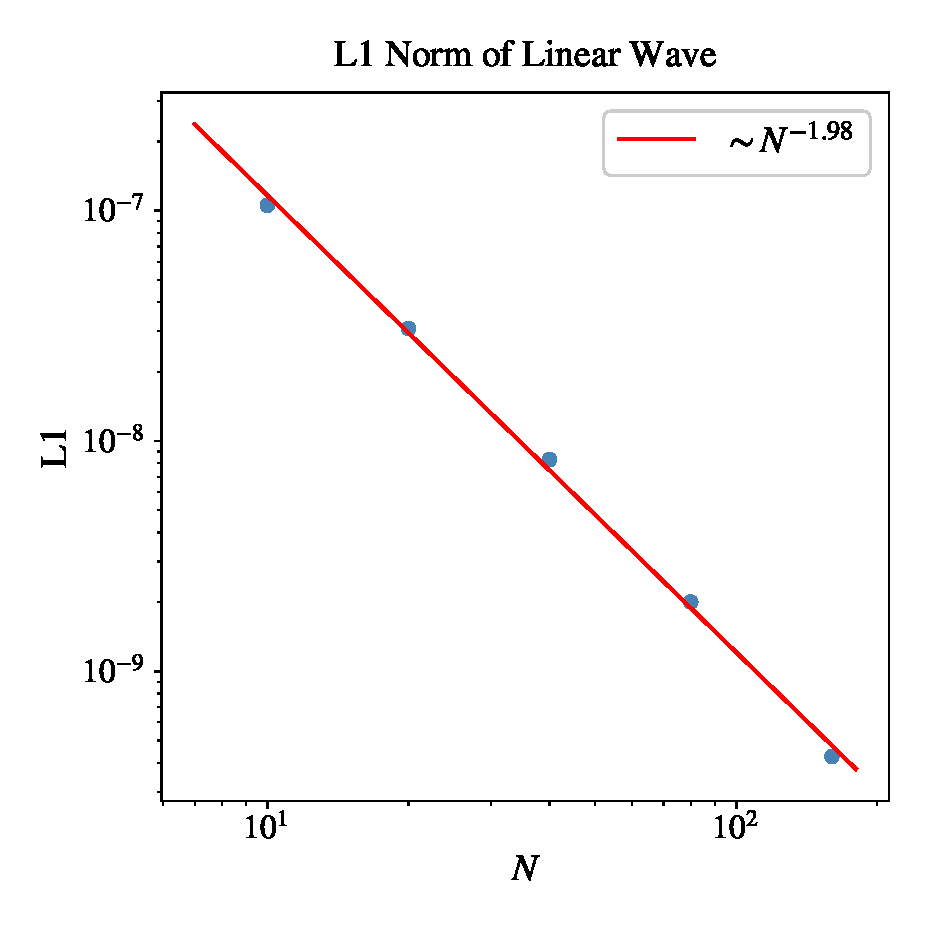
\includegraphics[width=0.4\textwidth]{figures/linear-wave-l1.eps}
        \caption{L1 norm of linear wave problem in 2d. Blue points are results
        of simulation from different resolutions overlaid by a linear fit showing
        the convergence is approximately second order. This example was produced by
        \textbf{linear\_wave\_2d.py} and \textbf{l1\_norm.py} scripts.}
        \label{fig.linear-wave}
    \end{center}
\end{figure}
Figure \ref{fig.linear-wave} shows the $L1$ norm as a function of grid cells per dimension.
As expected, the convergence rate is approximately second order in time and space for
this smooth problem. In the presence of shocks or other discontinuities it is not expected
to have such convergence.

\subsubsection{Sod shock-tube}
To examine the ability of the code to handle shock propagation we perform the Sod shock-tube 
problem \citep{toro-1997}. The problem consists of two different constant states at rest separated 
at the midpoint of the $x$ axis. A discontinuity exist in the density and pressure at that point. 
After $t=0$ the high density region flows into the lower density region. The flow produces a 
rarefaction, contact discontinuity, and a shock wave emanating from the density discontinuity. Thus, 
this problem creates a great test for the codes ability to capture the three wave types.

For our initial setup we use a unit box with reflective boundary conditions with density and pressure defined as
\begin{equation}
	\rho = \left\{
      \begin{array}{@{}ll@{}}
        	1.0 & \text{for}\ x \leq 0.5 \\
            0.125 & \text{for}\ x > 0.5
    	\end{array}\right.
\end{equation}
and
\begin{equation}
	P = \left\{
      \begin{array}{@{}ll@{}}
        	1.0 & \text{for}\ x \leq 0.5 \\
            0.1 & \text{for}\ x > 0.5
    	\end{array}\right.
\end{equation}
with $\gamma = 1.4$. The particles are laid out in a Cartesian grid and the simulation is evolved
until $t=0.15$. The number of particles per dimension is chosen to be $N=100$ and $N=45$ for 2D
and 3D respectively. This allows a comparison of a high and low resolution run.
\begin{figure}
    \begin{center}
        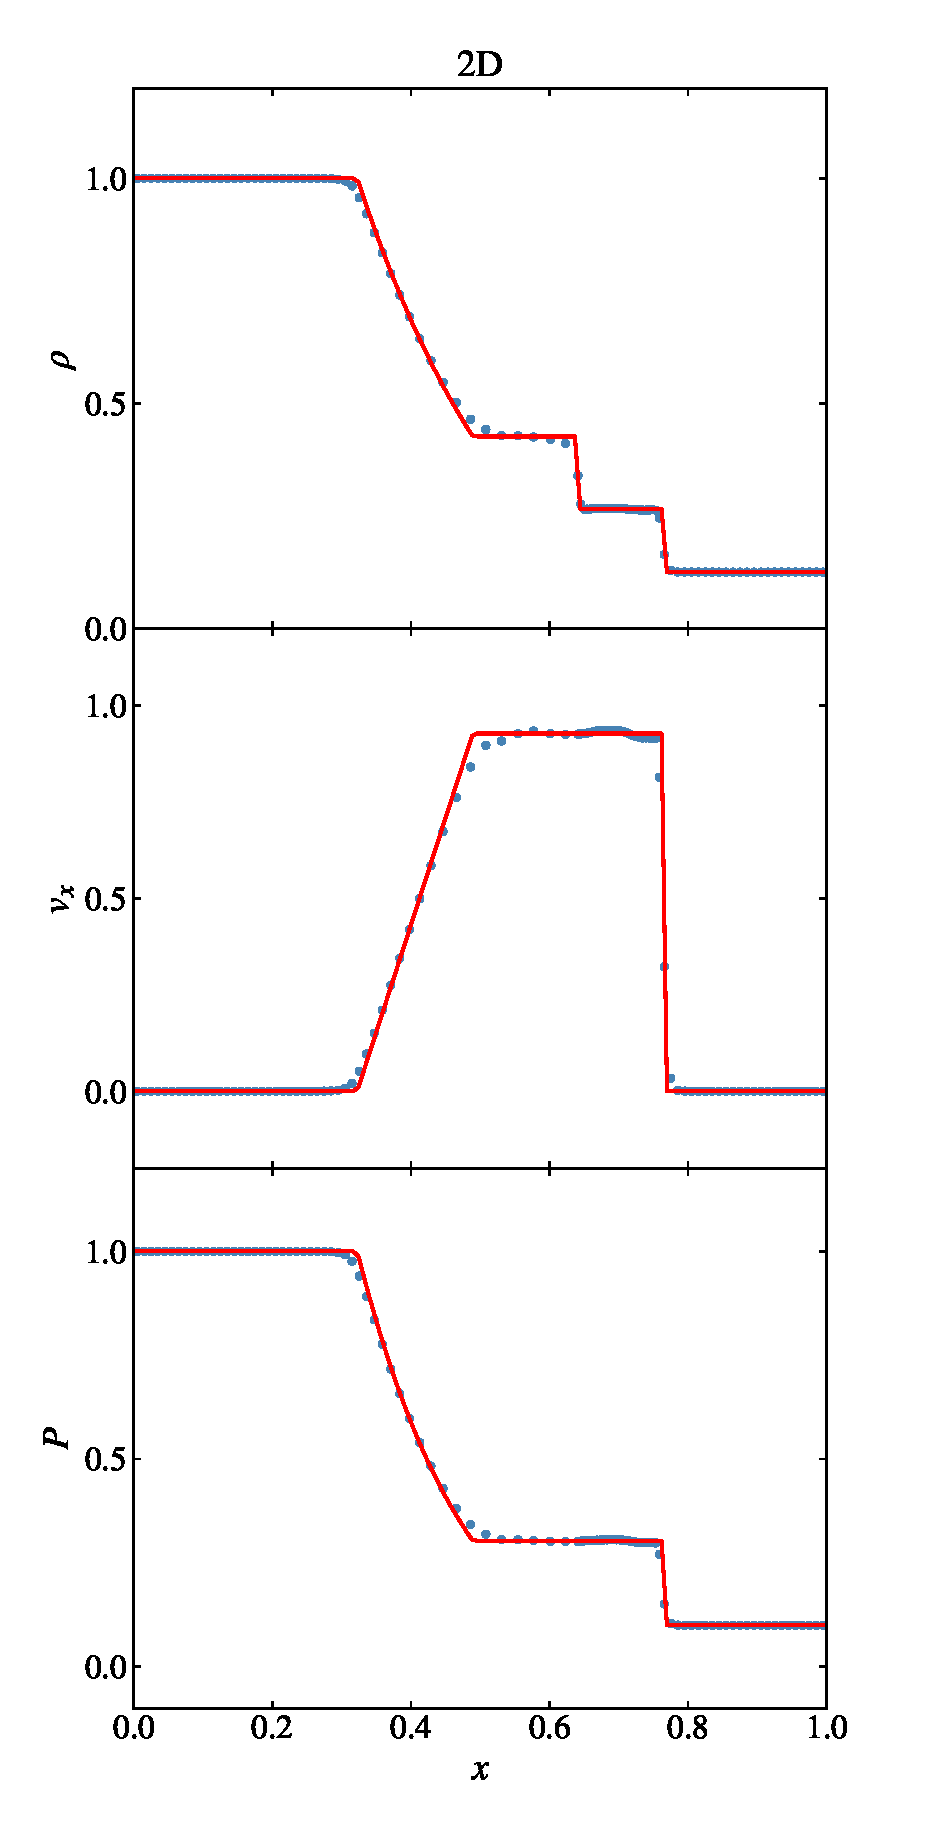
\includegraphics[width=0.4\textwidth]{figures/sod_2d.eps}
        \includegraphics[width=0.4\textwidth]{figures/sod_3d.eps}
        \caption{Profiles of density, $x$-component of velocity and pressure of the Sod 
        shock-tube simulation. Left: 2D run using a total of $100\times100$ particles. Right: 3D run 
        using a total of $45\times45\times45$, we only plot a slice of particles defined by $z=0$.
        Light blue points are the simulation while the red line is the exact solution.
        This example was produced by \textbf{sod\_2d\_cartesian.py},
        \textbf{sod\_3d\_cartesian.py}, \textbf{sod\_2d\_profiles.py}, and 
        \textbf{sod\_3d\_profiles.py} scripts.}
        \label{fig.sod}
    \end{center}
\end{figure}

Figure \ref{fig.sod} plots the particles density, $x$-component of velocity and pressure; only 
particles with $z=0$ are plotted in the 3D run for simplicity. The red line is the analytical 
solution. For the 2D simulation we can see the shock is well resolved as is the contact 
discontinuity. Further, the Lagrangian nature of the code can be seen as many particles have been 
squeezed between the contact discontinuity and the shock front while particles in the rarefaction 
have been spread out. For the 3D, lower resolution run, the code catches all three waves. Although, 
the contact discontinuity wave has been smoothed due to the lower number of particles.

\subsubsection{Explosion}
\begin{figure}
    \begin{center}
        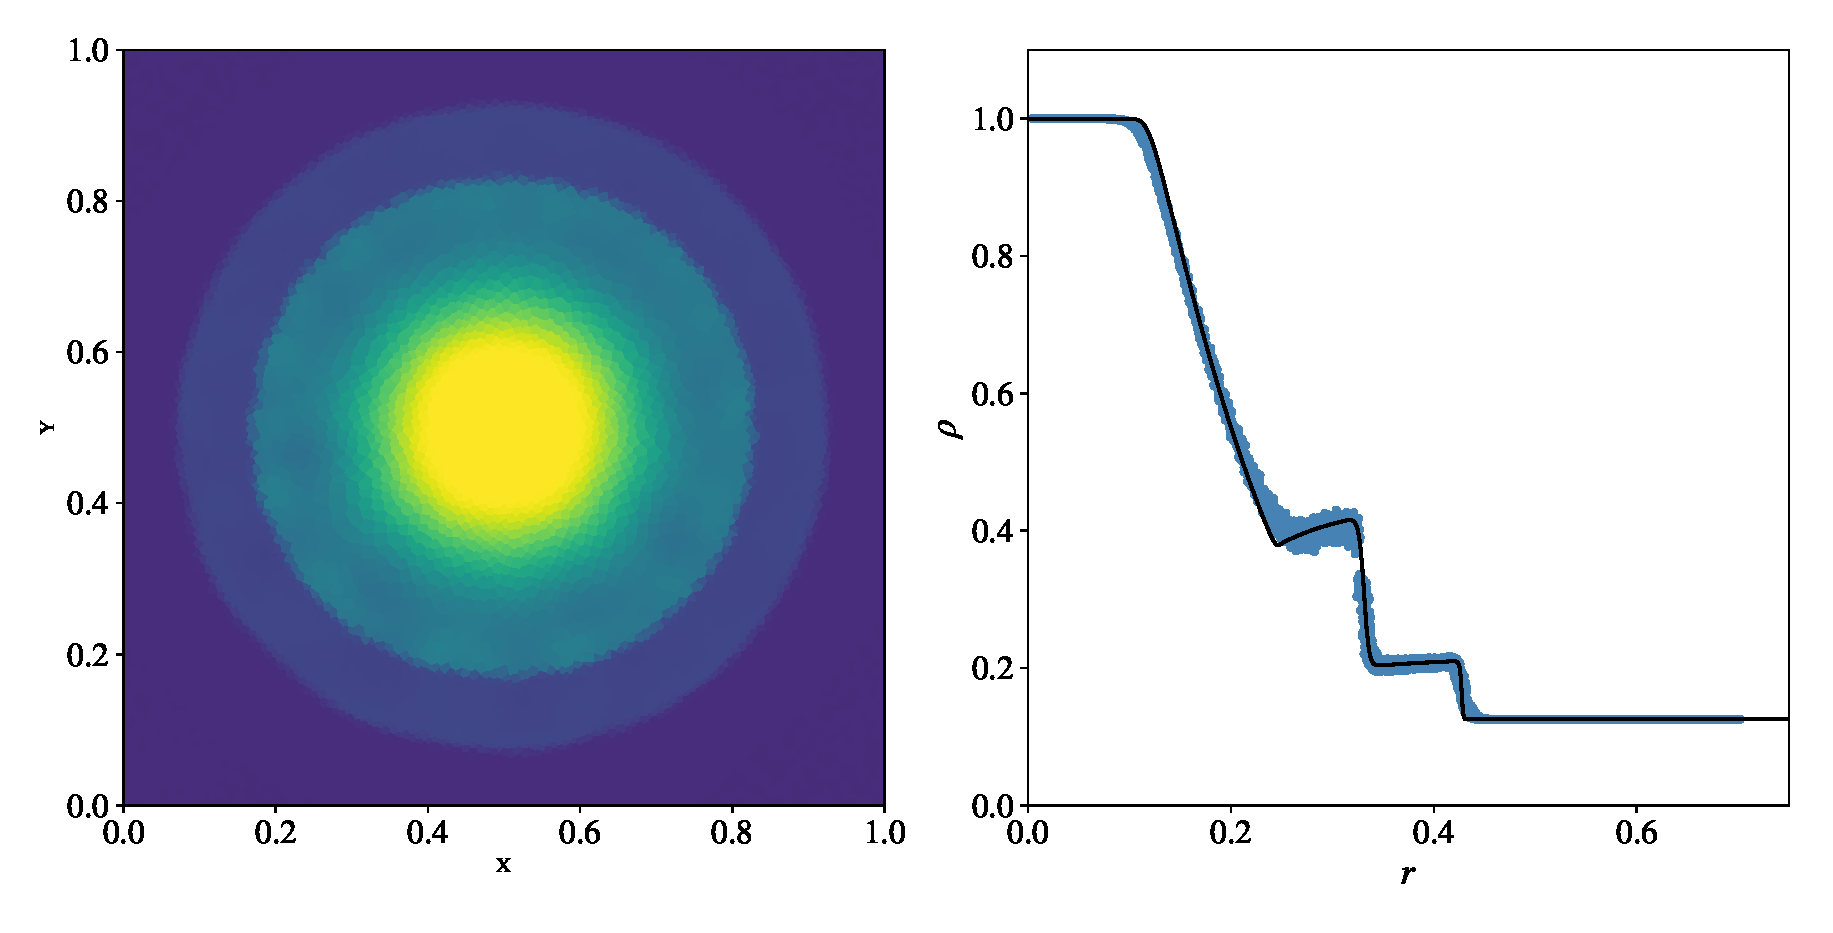
\includegraphics[width=0.8\textwidth]{figures/explosion_2d.eps}
        \caption{Density heatmap and radial profile of the Explosion problem. Left density
        heatmap, the irregular cells can been seen from the random initialization. Right
        radial density profile is an agreement with the exact solution in red.
        This example was produced by \textbf{explosion\_2d\_random.py} and 
        \textbf{explosion\_density\_panel.py} scripts.}
        \label{fig.explosion_2d}
    \end{center}
\end{figure}
An analog to the Sod problem is the 2D explosion problem \citep{toro-1997}. Like the Sod problem, 
the domain is partitioned into two constant states. However, the higher density region is now a 
circular region of radius $r$ centered in a unit box. Similar to the Sod problem, the initial 
conditions generate a shock, contact discontinuity and rarefaction wave. However, in this case
the waves are now a circular shock traveling radially outward, a circular contact
discontinuity traveling in the same direction, and a rarefaction wave traveling towards the
center.

We use the same values as the Sod problem except we restrict the higher density values onto
the center of domain with radius $r=0.25$. Further, instead of using a Cartesian grid we sample
particles uniformly for a unit square and perform 10 iterations of Lloyds algorithm. 

Figure \ref{fig.explosion_2d} shows the density map and density profile. Clearly, the cells
density matches the analytical solution in red. Further, the solution captures all three waves
even though the mesh was built in a random fashion. This an important difference over Eulerian
codes, since Lagrangian codes are not constrained to any initial particle placement. Therefore
one can reach better accuracy by placing the particles in way that exploits the problem. We will
see a later example of this in the Evrards problem, see Section \ref{sec.evrards}.

\subsubsection{Gresho vortex}
Our next problem will test stability of the code in maintaining equilibrium. \cite{Gresho90}, 
introduced an interesting problem to test for conservation of angular momentum. A vortex in a unit 
2D box with constant density $\rho=1$ is setup with the following angular velocity
\begin{equation}
	v_\phi (r) = \left\{
      \begin{array}{@{}ll@{}}
        	5r & \text{for}\ 0 \leq r < 0.2 \\
            2-5r & \text{for}\ 0.2 \leq r < 0.4 \\
            0 &\text{for}\ \geq 0.4
    	\end{array}\right.
\end{equation}
The angular velocity of the vortex grows linearly as one moves radially outward from
the center until midway of the disk. Then the velocity decreases linearly until it
vanishes at the rim of the disk. This produces triangular shape velocity profile.
The corresponding pressure is
\begin{equation}
	P(r) = \left\{
      \begin{array}{@{}ll@{}}
        	5 + 25/2r^2 & \text{for}\ 0 \leq r < 0.2 \\
            9+25/2r^2 - 20r + 4\ln(r/0.2) & \text{for}\ 0.2 \leq r < 0.4 \\
            3 + 4\ln(2) &\text{for}\ \geq 0.4.
    	\end{array}\right.
\end{equation}
The pressure is chosen such that the pressure gradients balance the centrifugal forces
generated by the rotation. Thus producing a solution that is independent of time.
\begin{figure}
    \begin{center}
        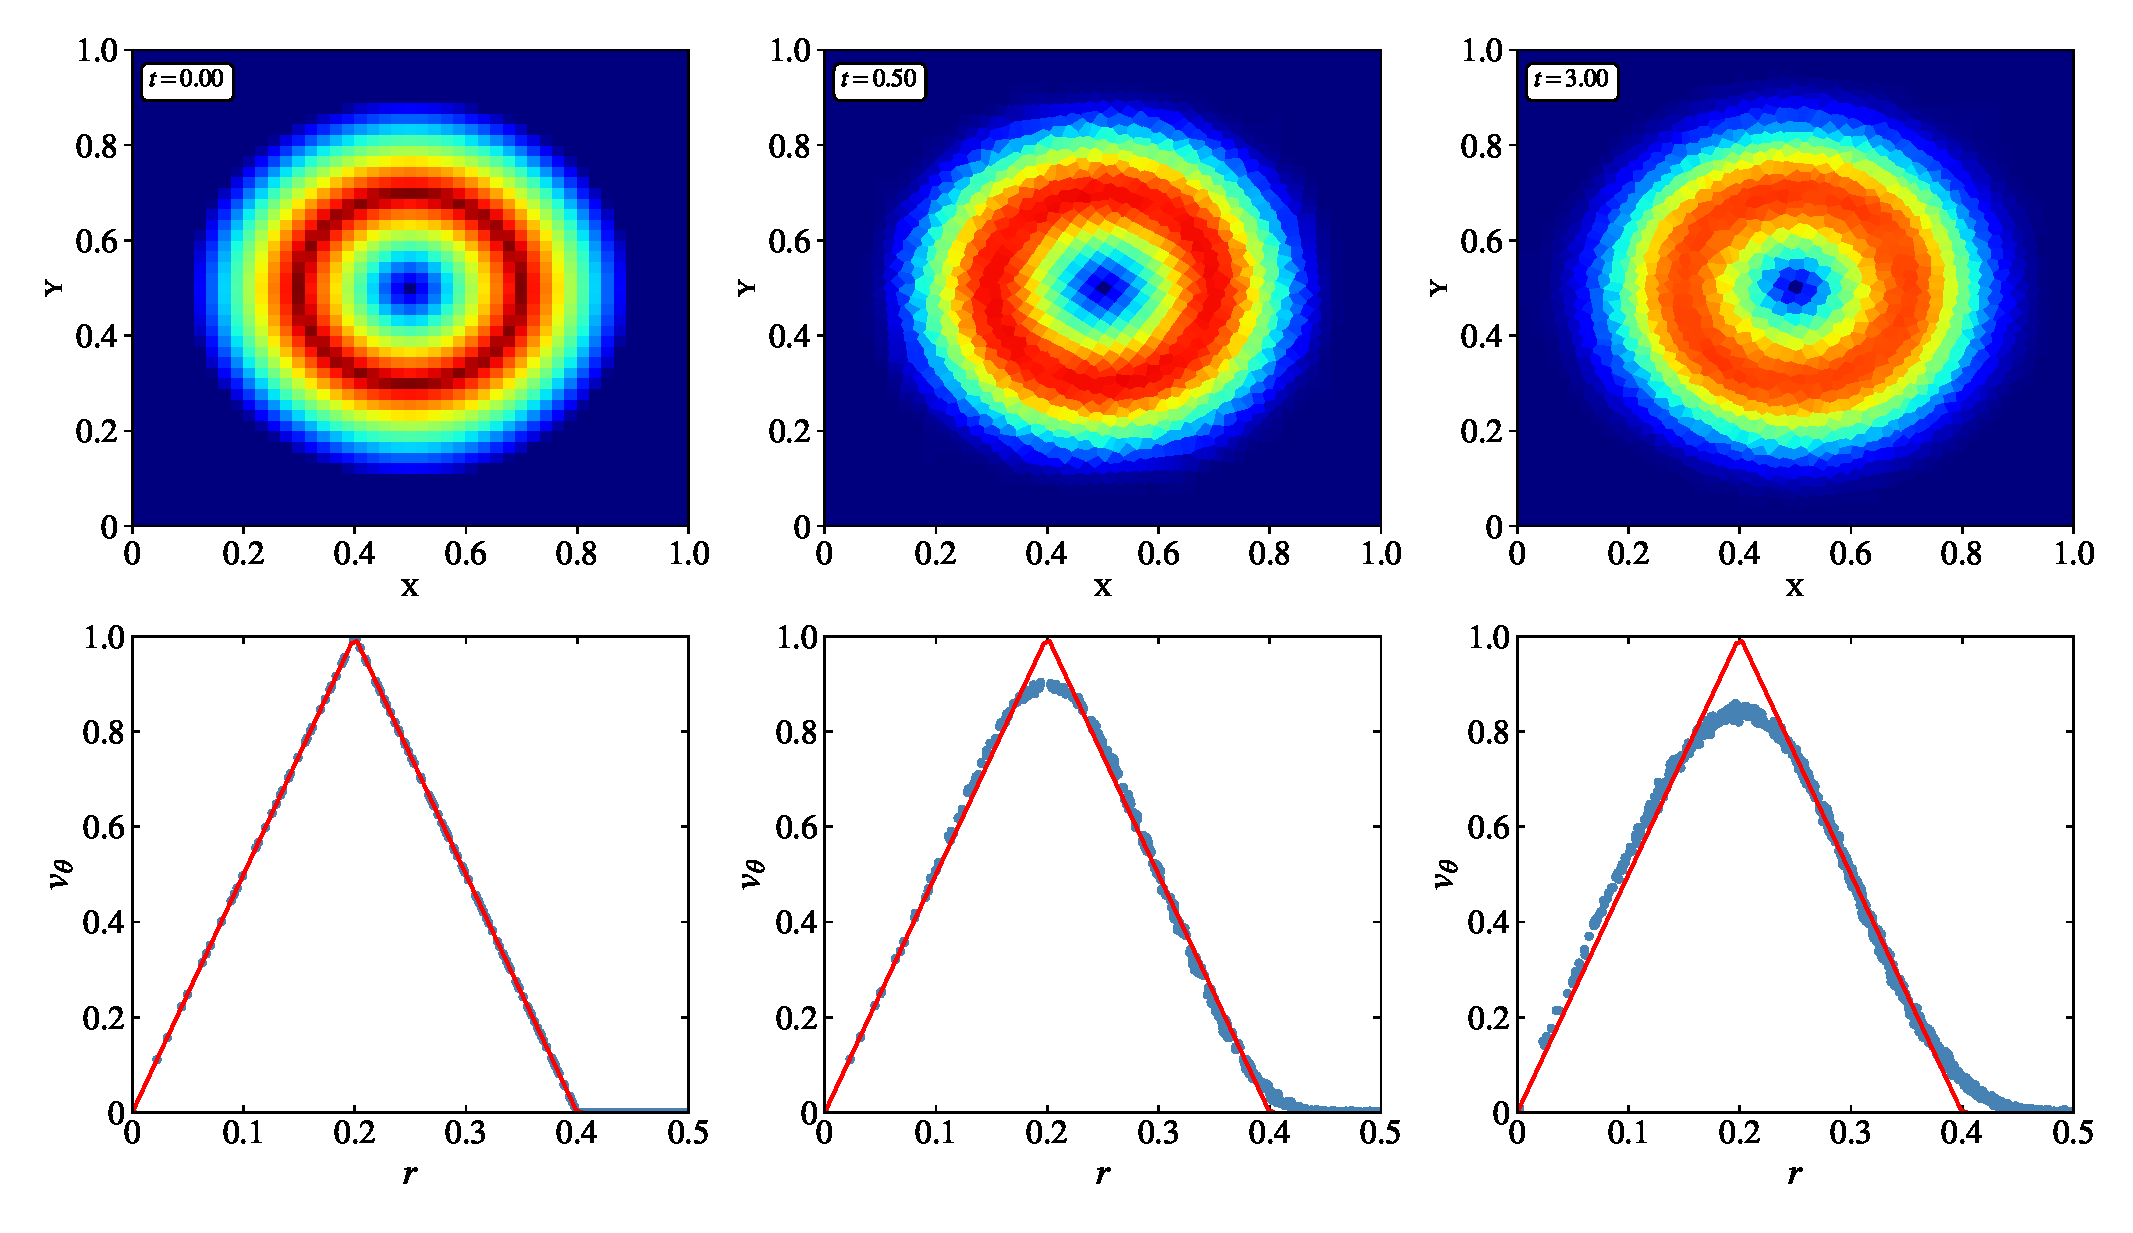
\includegraphics[width=0.8\textwidth]{figures/gresho_vortex.eps}
        \caption{Heatmap and radial profile of azimuthal velocity. Top row: time evolution
        of the cells at times $t=0.0, 0.5, 3.0$. Bottom row: corresponding radial profile of 	
        azimuthal velocity. As the simulation evolves the systems remains in equilibrium.
        This example was produced by \textbf{gresho\_2d\_cartesian.py} and 
        \textbf{gresho\_density\_panel.py} scripts.}
        \label{fig.gresho_vortex}
    \end{center}
\end{figure}
Figure \ref{fig.gresho_vortex} shows three snapshots at $t=0.0, 0.5, 3.0$ of the azimuthal
velocity. The top row is a 2d heat map while the bottom row is a radial profile. At time $t=0$
all the cells are rectangular. As the system evolves the cells that are rotating become irregular 
polygons. There is a small amount of velocity smoothing at the initial largest velocities and at
the rim of the vortex. However, it is evident that the system stays in equilibrium.

\subsubsection{Sedov-Taylor}
Another test that generates a shock is the Sedov-Taylor blast wave problem \citep{Sedov1959}. In 
this problem a homogeneous gas is injected with a large amount of energy in a point-like region at 
the center of the domain. A spherical shock is created emanating from the center. The shock 
propagates radially outward sweeping mass into a thin shell and creating a cavity behind the shock. 
The problem has a well known analytical self-similar solution; see \cite{Sedov1959} for details. 
Applying the Rankine–Hugoniot at the shock front the density jumps to a maximum compression of
\begin{equation}
	\rho_{\mathrm{max}}/\rho = (\gamma + 1)/(\gamma - 1),
\end{equation}
for $\gamma = 5/3$ this amounts to a max value of 4.

We consider the 2D and 3D case. A unit box is setup with particles in a Cartesian grid of size
$45\times 45$ and $45 \times 45 \times 45$ for 2D and 3D respectively. The stationary gas has
a constant density of $\rho = 1.0$ and pressure $P = 10^{-6}$ with $\gamma=5/3$. The simulation is
allowed to evolve to time $t=0.06$.
\begin{figure}
    \begin{center}
        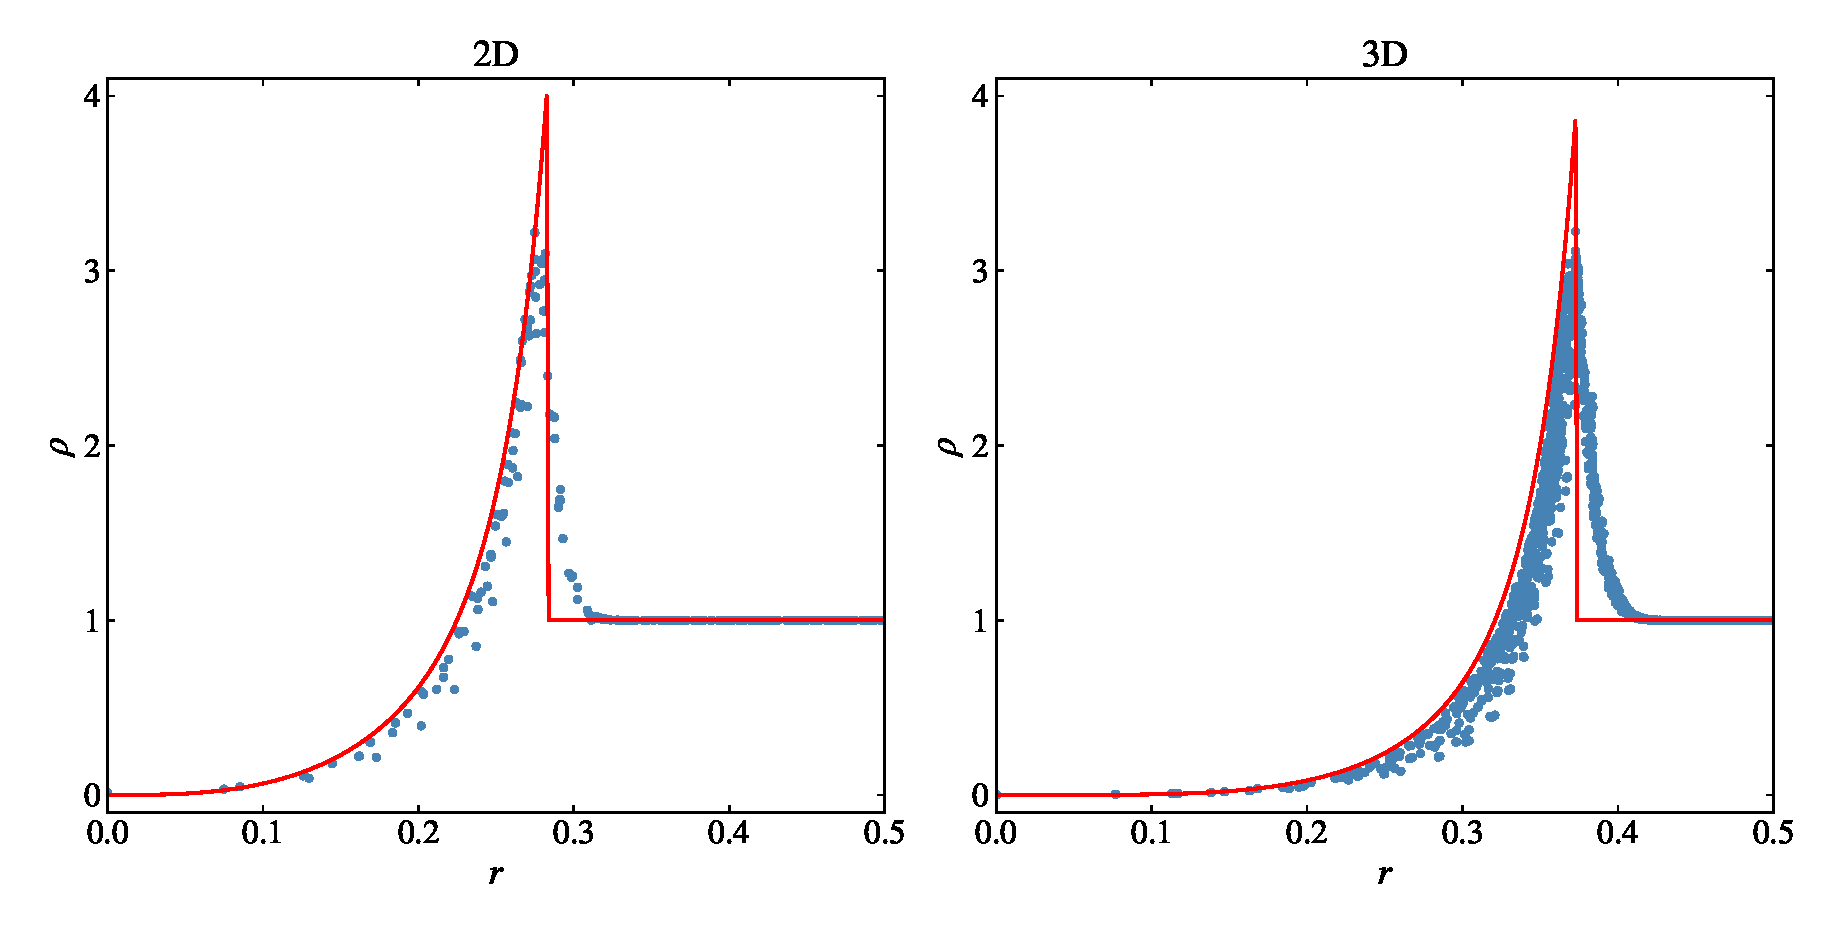
\includegraphics[width=0.8\textwidth]{figures/sedov_compare.eps}
        \caption{Density profile of Sedov-Taylor blast wave problem. Left: 2D version with an 
        initially Cartesian mesh of $45 \times 45$. Right: 3D version with an initially 
        Cartesian mesh of $45 \times 45 \times 45$; only a random sample of $45\times45$ is
        plotted for simplicity. Light blue points are the density at radius $r$ 
        from the center of the explosion while the red line is the exact solution.
        This example was produced by \textbf{sedov\_2d\_cartesian.py},
        \textbf{sedov\_3d\_cartesian.py}, and \textbf{sedov\_density\_compare.py} scripts.}
        \label{fig.sedov}
    \end{center}
\end{figure}
Figure \ref{fig.sedov} shows the cell density as a function of radial distance from the center of 
the explosion. It is noted that shock is well resolved by the cells as the mesh has deformed in such 
a way that the shock front contains a large amount of cells which is evident in
Figure \ref{fig.sedov_panel}.
\begin{figure}
    \begin{center}
        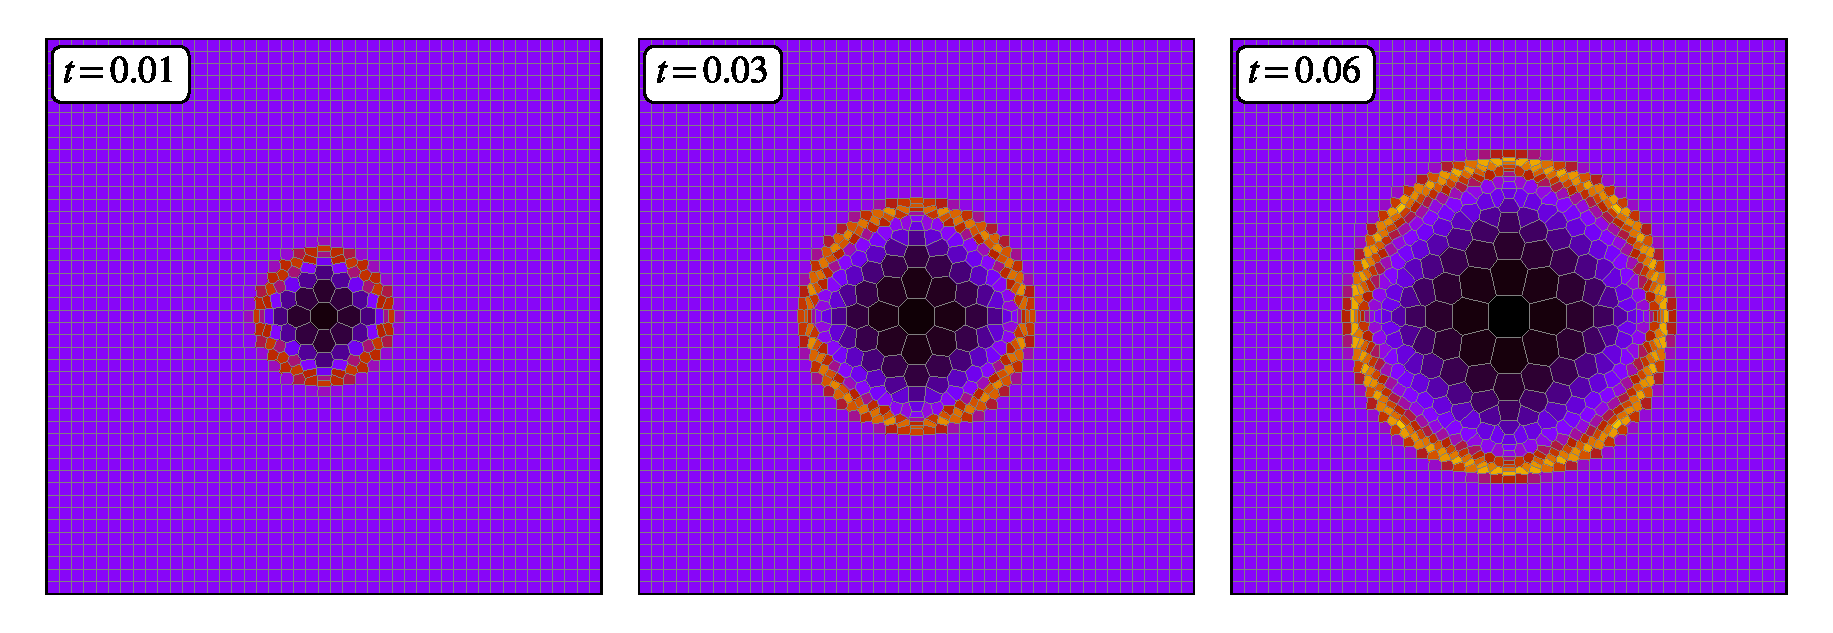
\includegraphics[width=0.8\textwidth]{figures/sedov_panel.eps}
        \caption{Evolution of the density at several times. The initial cell with the energy
        imparted remains stationary as the cells around it move radially outward. The cells at
        the shock are compressed allowing for better resolution. This example was produced by 
        \textbf{sedov\_2d\_cartesian.py} and \textbf{sedov\_density\_panel.py} scripts.}
        \label{fig.sedov_panel}
    \end{center}
\end{figure}
The center cell, where the energy is deposited, remains stationary while the
cells around it move radially outward. The cells exterior to the shock remain
stationary until they are swept and compressed by the shock.

\subsubsection{Kelvin-Helmholtz instability}
For our last hydrodynamic test we consider the Kelvin-Helmholtz (KH) instability. This
problem consist of a shear-flow where a single mode is excited by a velocity perturbation.
Specifically, two layers with different densities are initially in pressure equilibrium. 
Each layer flows in the opposing direction and receives a velocity perturbation perpendicular
to the interface. The perturbation grows exponentially and produces structures which
are called KH instabilities. A difficulty of this problem is that
numerical errors, noise, and resolution seed spurious small structure \citep{Lecoanet2016}
making direct comparisons a difficult endeavor. However, we can use this problem to
visually verify the characteristics of the problem are maintained
and leave the exact detail treatment to the next revision of the code.

We follow \cite{Springel2010} and setup a unit periodic box with density
\begin{equation}
	\rho = \left\{
      \begin{array}{@{}ll@{}}
            2 & \text{for}\ y < 0.25 \\
            1 & \text{for}\ 0.25 \leq y \leq 0.75\\
            2 & \text{for}\ 0.75 < y,
    	\end{array}\right.
\end{equation}
$x$-component of velocity
\begin{equation}
	v_x = \left\{
      \begin{array}{@{}ll@{}}
            -0.5 & \text{for}\ y < 0.25 \\
            0.5 & \text{for}\ 0.25 \leq y \leq 0.75\\
            -0.5 & \text{for}\ 0.75 < y,
    	\end{array}\right.
\end{equation}
and $y$-component of velocity
\begin{equation}
	v_y(x, y) = w_0 \mathrm{sin}(4\pi x) \left(\exp\left(-\frac{(y-0.25)^2}{2\sigma^2}\right) +
    	\exp\left(-\frac{(y-0.75)^2}{2\sigma^2}\right)\right)
\end{equation}
where $w_0=0.1$ and $\sigma=0.05/\sqrt{2}$. The pressure is set to $P=2.5$, $\gamma=5/3$
and the simulation is evolved until time $t=2$.
\begin{figure}
    \begin{center}
        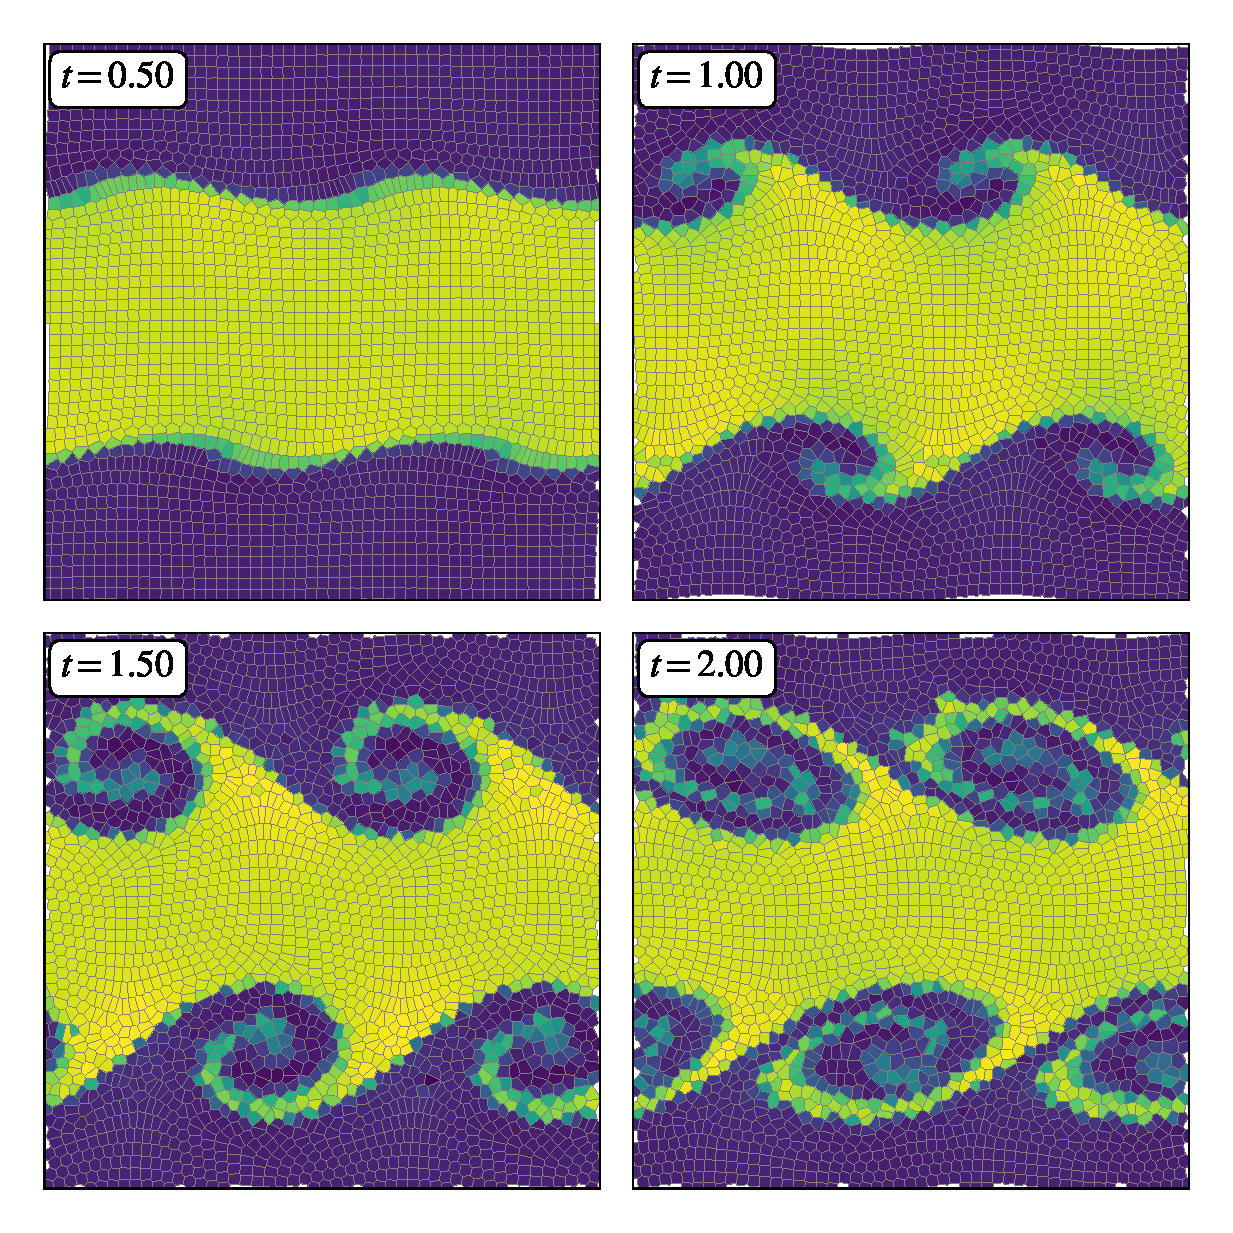
\includegraphics[width=0.8\textwidth]{figures/kelvin.eps}
        \caption{Evolution of the density at several times in the KH problem. We see the common
        traits of KH evolution, KH billows and mixing. This example was produced by 
        \textbf{kelvin\_helmholtz\_2d\_cartesian.py} and 
        \textbf{kelvin\_helmholtz\_density\_panel.py} 
        scripts.}
        \label{fig.kelvin}
    \end{center}
\end{figure}

Figure \ref{fig.kelvin} shows the density field for several selected times. Comparing with
Springel, visually we conclude that the results are in close agreement. The formation of the
Kevlin Helmholtz billows and mixing of both fluids at each time are similar.

\subsection{Gravity Tests}
\subsubsection{Two body}
Our first problem, in testing our gravity solver, is a simple two body problem where two particles
interact with each other through their gravitational force. Although, this problem does not really test the 
implementation of the gravity tree, since only two leaves will be constructed
in the tree and it is most likely that the leaves will interact with each other bypassing the node 
moments, it does test the gravity kernel and stability of the leap frog integrator.

For this problem an exact solution exists by reducing it to a single body. Given
two particles with masses $m_1$ and $m_2$ with positions $\vec{r}_1$ and $\vec{r}_2$ the equation of motion for
the reduced mass
\begin{equation}
	\frac{1}{\mu} = \frac{1}{m_1} + \frac{1}{m_2}
\end{equation}
is
\begin{equation}
	\mu\frac{d^2 \vec{r}}{dt^2} = -\frac{G m_1 m_2}{r^2}\hat{r},
    \label{eq.reduced-force}
\end{equation}
where $\vec{r}$ is the separation vector $\vec{r}_1 - \vec{r}_2$. Equation \ref{eq.reduced-force} can be
transformed to polar coordinates giving the solution
\begin{equation}
	r = \frac{a(1-\epsilon^2)}{1-\epsilon cos(\theta)}
\end{equation}
for initial conditions $a$ and $\epsilon$. The overall system evolves with a period of
\begin{equation}
    T = \sqrt{\frac{4\pi^2 a^3}{G m}},
\end{equation}
where $m=m_1 + m_2$. To recover the particles positions, a final transformation
of the form
\begin{equation}
	\begin{array}{rcl}
		\vec{r}_1 & = & \frac{m_1}{m}\vec{r}\\
    	\vec{r}_2 & = & -\frac{m_2}{m}\vec{r}
    \end{array}
\end{equation}
is used. The initial position and velocity of the particles can be parameterized by $a$,
$\epsilon$ and $q=m_1/m_2$
\begin{equation}
	\begin{array}{rcl}
    	\vec{r}_1 & = & a\frac{1-\epsilon}{1+q} \hat{x}\\
        \vec{v}_1 & = & \frac{1}{1+q}\sqrt{\frac{1+\epsilon}{1-\epsilon}}\sqrt{\frac{Gm}{a}} \hat{y}\\
        \vec{r}_2 & = & -q \vec{r}_1\\
        \vec{v}_2 & = & -q \vec{v}_1.
    \end{array}
\end{equation}

We setup the particles with parameter values $a=0.5$ and $\epsilon=0.25/0.75$ with $G=1$ and allow
the simulation to evolve for 10 periods. The time step is held fixed with a value of $dt=T/1000$.
In Figure \ref{fig.two_body} we show the trajectory for both particles as well as the evolution of
the relative total energy error. We clearly see that both trajectories remain along the exact solution
signifying the stability of the leap frog integrator. Further we see that the relative total energy
error remains bounded by zero and $-1.1\times10^{-4}$ indicating that the total energy remains
accurately conserved.
\begin{figure}
    \begin{center}
        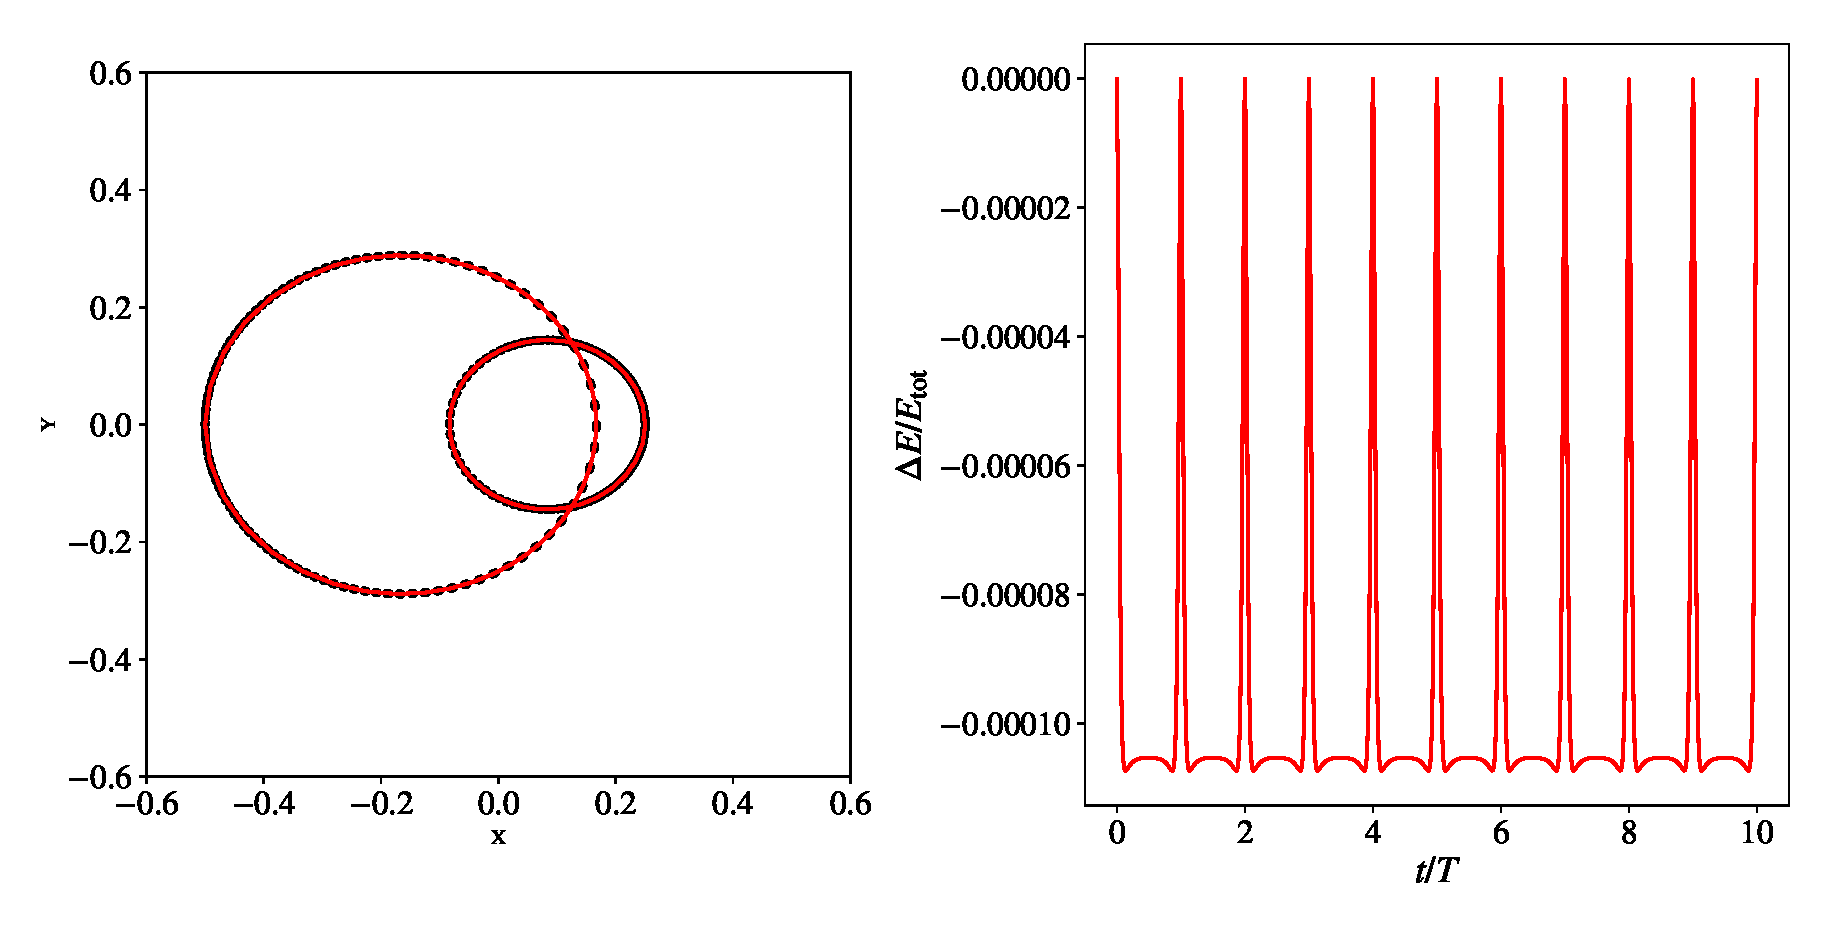
\includegraphics[width=0.9\textwidth]{figures/two_body.eps}
        \caption{Left: Trajectories of the two body problem for ten periods. Clearly
        both particles remain in their orbital path shown in red signifying the stability
        of the leap frog integrator. Right: Corresponding relative total energy error.
        The total energy remains accurately conserved as the worst relative error is
        $-1.1\times10^{4}$.}
        \label{fig.two_body}
    \end{center}
\end{figure}

\subsubsection{Plummer sphere}
The Plummer sphere cite is a model that can be used to describe the distribution of stars and in a cluster
and is commonly used to test gravity solvers. The Plummer sphere, i.e. a polytrope of index 5,
has a density profile of the from
\begin{equation}
	\rho (r) = \frac{3 M}{4\pi R^3} \left(1 + (r/R)^2\right)^{-5/2},
    \label{eq.plummer}
\end{equation}
where $M$ is the total mass of the cluster and $R$ is a scale parameter which sets the
size of the cluster. The system is in steady state with an isotropic velocity distribution.
To test our gravity solver, we initialize our particles with the given distributions and
advance the system in time. We expect the system to stay in steady state therefore we compare
the initial density distribution with the final state of the system.

For our test we chose the parameters of the Plummer sphere to be $M=1,000$ and $R=1$ with
$G=1$. We then sampled 10,000 particles using the the rejection technique outlined in
cite to set the position and velocities. The system is allowed to evolve to time $t=1$
which is roughly ten dynamical times. The gravitational tree used an opening angle 0.4
and smoothing parameter of 0.03.
\begin{figure}
    \begin{center}
        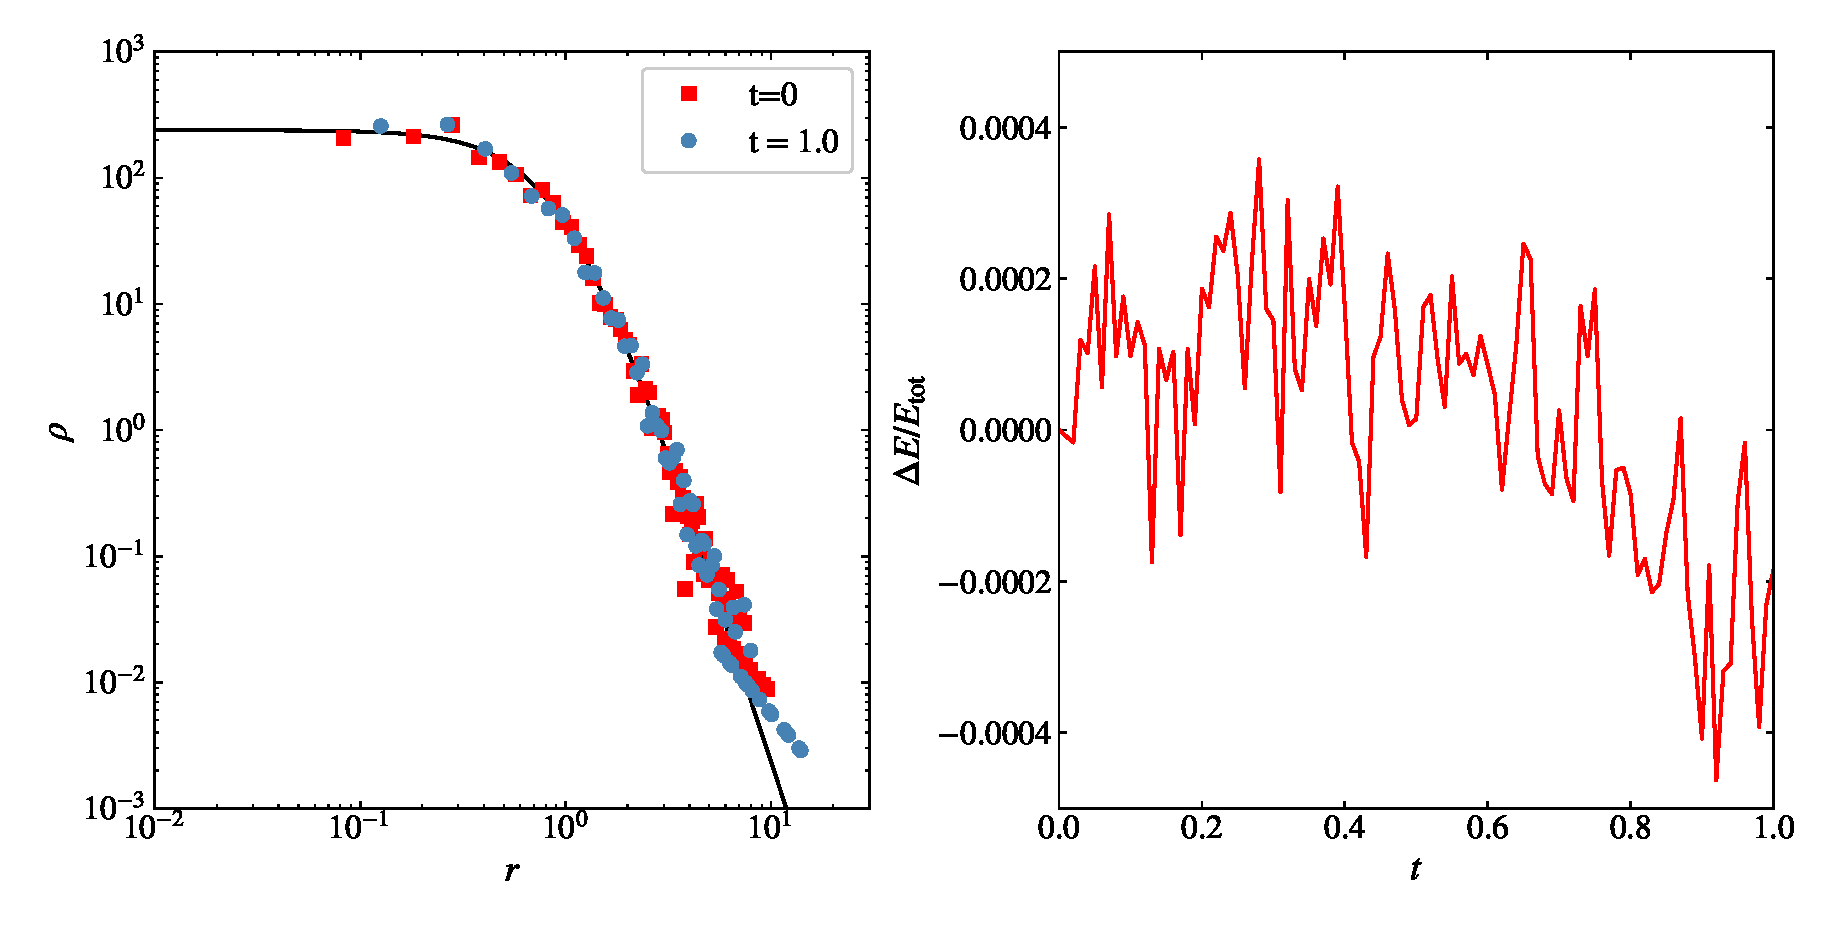
\includegraphics[width=0.9\textwidth]{figures/plummer.eps}
        \caption{Density profile of Sedov-Taylor blast wave problem. Left is the 2D version with an initially
        Cartesian mesh of $45 \times 45$. Right is the 3D version with an initially Cartesian mesh of 
        $45 \times 45 \times 45$. Light blue points are the density a radius $r$ from the center of the explosion
        while the red line is the exact solution.}
        \label{fig.plummer}
    \end{center}
\end{figure}
The left panel of Figure \ref{fig.plummer} shows the density profile at the initial and final 
time of the simulation with equation \ref{eq.plummer} overlaid as a reference. The density is calculated
by dividing the space by spherical shells, binning and dividing by the volume. It is clearly shown that
at the final time the particles remain in steady state with their positions matching the initial
distribution. The right panel of \ref{fig.plummer} shows the evolution of the relative error of the
total energy of the system. The error stays well below $5\times 10^{-4}$ with a final error of
$2\times 10^{-4}$, entailing the solver has accurately maintained the total energy.

\subsubsection{Rayleigh Taylor}
Our first hydrodynamic problem to include gravity is the Rayleigh Taylor instability problem.
The problem consists of dense fluid over a lighter fluid in the presence of a uniform 
vertical gravitational field. A perturbation is placed in the vertical direction causing the
dense field to sink while the lighter rises through buoyancy.

A rectangular domain of the size $[1\times3]$ is chosen with the gravitational force in the
$y$-direction with strength of $g=1$. The initial setup of the density
is
\begin{equation}
	\rho = \left\{
      \begin{array}{@{}ll@{}}
            1 & \text{for}\ y \leq 1.5 \\
            2 & \text{for}\ 5 > 1.5,
    	\end{array}\right.
\end{equation}
while the pressure is
\begin{equation}
	P = \left\{
      \begin{array}{@{}ll@{}}
            10 - y & \text{for}\ y \leq 1.5 \\
            11.5 + 2(y-1.5) & \text{for}\ 5 > 1.5,
    	\end{array}\right.
\end{equation}
such that the system is initially in hydrostatic equilibrium. A perturbation is applied
to the $y$-velocity
\begin{equation}
	v_y = \mathrm{cos}\left(2\pi x\right)\exp{-(y-1.5)^2/0.1}
\end{equation}
We set $\gamma=1$ and let the system evolve to $t=3.0$. Although without an implementation
of viscosity there is no one correct solution that all codes converge to. However, we can
visually inspect if our simulation share the same characteristics of another established
code. In Figure we that the single mode is very similar to the results from cite
\begin{figure}
    \begin{center}
        \includegraphics[width=0.6\textwidth]{figures/rayleigh_compare.eps}
        \caption{Density profile of Sedov-Taylor blast wave problem. Left is the 2D version with an initially
        Cartesian mesh of $45 \times 45$. Right is the 3D version with an initially Cartesian mesh of 
        $45 \times 45 \times 45$. Light blue points are the density a radius $r$ from the center of the explosion
        while the red line is the exact solution.}
        \label{fig.rayleigh}
    \end{center}
\end{figure}

We see the mode has the characteristics of

\subsubsection{Evrard Collapse}
\label{sec.evrards}
The final test is the Evrards collapse problem which tests the coupling of self-gravity and hydrodynamics.
The problem consists of an initially non-rotating isothermal gas sphere with mass $M=1$ and radius $R=1$
with a density 
\begin{equation}
	\rho(r) = \left\{
      \begin{array}{@{}ll@{}}
            1/\left(2\pi r\right) & \text{for}\ r \leq 1 \\
            0 & \text{for}\ r > 1
    	\end{array}\right.
\end{equation}
and pressure
\begin{equation}
	P(r) = \left\{
      \begin{array}{@{}ll@{}}
            0.05 /\left(3\pi r\right) & \text{for}\ r \leq 1 \\
            0 & \text{for}\ r > 1.
    	\end{array}\right.
\end{equation}
The gravitational constant is set to $G=1$ and $\gamma=5/3$. The evolution of the sphere begins
with mass falling towards the center due to self-gravity. The pressure at the center rises and
produces a shock traveling outward through the in-falling gas. The final state of the gas is a
spherical distribution in hydrostatic virial equilibrium.

We setup an initial Cartesian grid of size $33\times 33\times 33$ particles. Due to the nature
of the $1/r$ density profile, a Cartesian mesh will not resolve the high density values unless
the resolution is sufficiently increased. However we have complete freedom on how to the particles
are initially setup. Therefore, we transform particles radially inside the sphere by the following
\begin{equation}
    r_{\mathrm{new}} = r_{\mathrm{old}}^{3/2}.
\end{equation}
Such a transformation maps a grid of equally spaced particles with uniform density to
a set of particles spaced in such a way that the uniform density follows a $1/r$ profile. 
\begin{figure}
    \begin{center}
        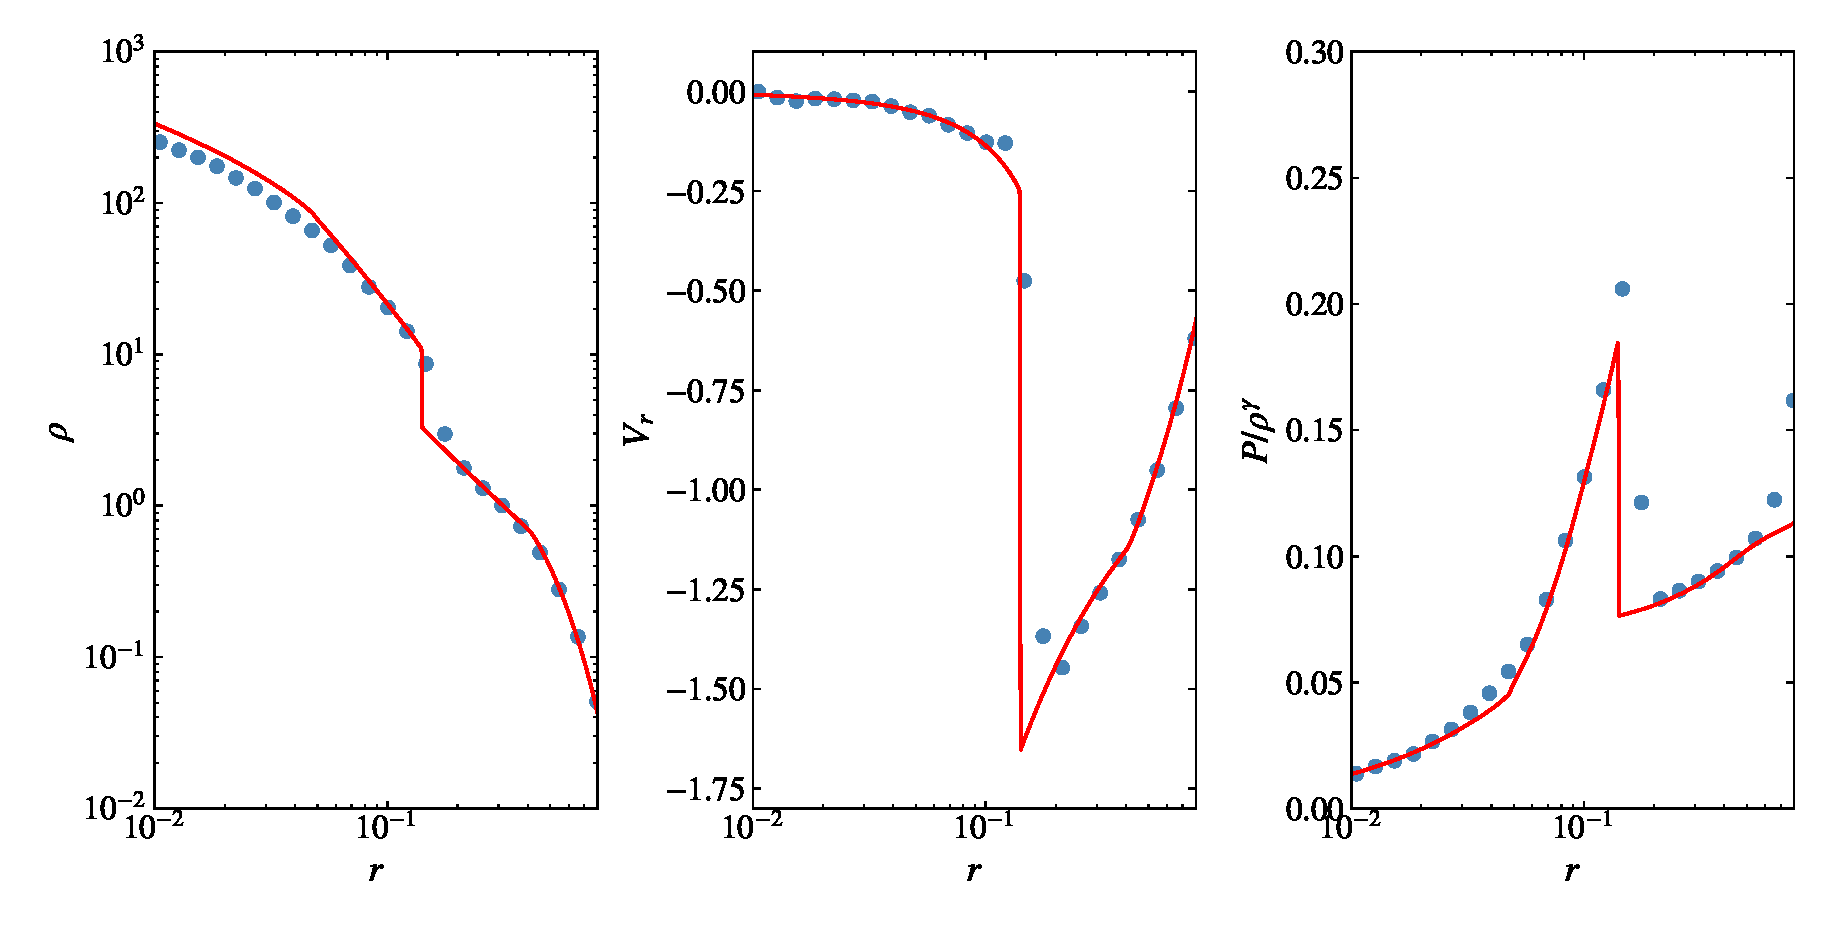
\includegraphics[width=0.9\textwidth]{figures/evrard.eps}
        \caption{Density profile of Sedov-Taylor blast wave problem. Left is the 2D version with an initially
        Cartesian mesh of $45 \times 45$. Right is the 3D version with an initially Cartesian mesh of 
        $45 \times 45 \times 45$. Light blue points are the density a radius $r$ from the center of the explosion
        while the red line is the exact solution.}
        \label{fig.evrard}
    \end{center}
\end{figure}

The radial averaged density, radial velocity and entropy are shown in Figure at time $t=0.81$
when the shock has formed and is traveling outward. We see all profiles adequately follow the
exact solution in red for this low resolution run. Further we see that there is significant
error in the conservation of energy Figure. This is expected as noted by Springel. The 
discrepancy arises from the gravitational work term which ignores the motion of mass
exchanged by adjacent cells. Springel proposed a new formulation for then energy equation
that results in better energy conservation. This updated method will be added in the next
revision of the code.
\begin{figure}
    \begin{center}
        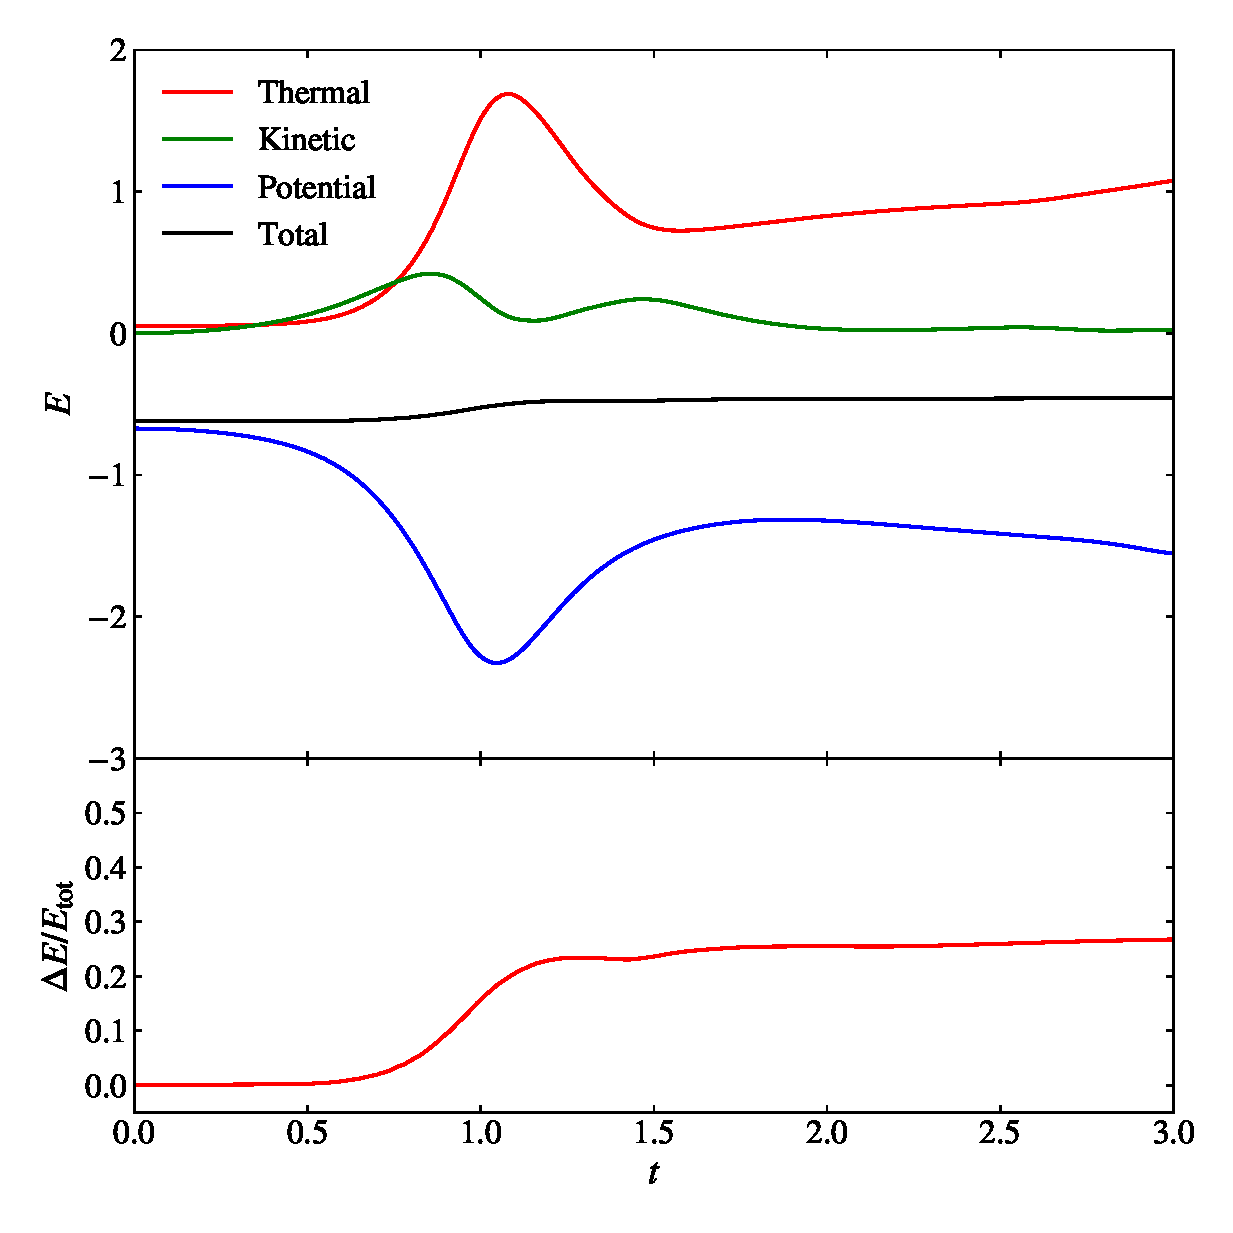
\includegraphics[width=0.6\textwidth]{figures/evrard_energy.eps}
        \caption{Density profile of Sedov-Taylor blast wave problem. Left is the 2D version with an initially
        Cartesian mesh of $45 \times 45$. Right is the 3D version with an initially Cartesian mesh of 
        $45 \times 45 \times 45$. Light blue points are the density a radius $r$ from the center of the explosion
        while the red line is the exact solution.}
        \label{fig.evrard_energy}
    \end{center}
\end{figure}


%\section{Fluid methods}
%\label{sec.fluids}
%
%\input{numerical-ppm}
%\subsection{Hydrodynamics and Magnetohydrodynamics: MUSCL with Dedner cleaning}
\label{sec.num.hydro-muscl}

The second method we describe is a MUSCL-based solver than can be used
in both HD and MHD modes.  The description here will be very brief
both because the ideas are similar to those described in the previous
section, and because this implementation has previously been described
in more detail elsewhere \citep{WangAbelZhang08, WangAbel09}.

Much like the PPM solver, we have three basic steps: the first is reconstruction of the variables, the second is a solution of the Riemann problem, and the third is is updating the conserved quanties with the fluxes as written above. For the reconstruction scheme we have implemented only the simple piecewise linear reconstruction \citep{1979JCoPh..32..101V, 1985JCoPh..59..264C}, with options for both primitive and conservative variable reconstruction. The available Riemann solvers are HLL, HLLC, and HLLD, as described earlier.

To more clearly describe the Dedner divergence cleaning modifications,
we write the equations of compressible inviscid hydrodynamics in the
form of conservation laws as,

\begin{equation}
 \frac{\partial{U}}{\partial{t}} +
 \frac{\partial{F^x}}{\partial{x}} + \frac{\partial{F^y}}{\partial{y}} + \frac{\partial{F^z}}{\partial{z}}= 0, \label{hydro}
\end{equation}

The conserved variable $U$ is given by

\begin{equation}
 U = (\rho, \rho v_x, \rho v_y, \rho v_z, \rho E)^{T},
\end{equation} 

where $\rho$ is density, $v_i$ are the three components of velocity
for $i={x,y,z}$, $E=v^2/2 + e$ denotes the specific total energy and $e$ the
specific internal energy (note that in this section only, we use the specific
energy).

For the generalized Lagrange multiplier (GLM) formulation of the MHD
equations \citep{2002JCoPh.175..645D}, we consider these 
conserved variables

\begin{equation}
 U = (\rho, \rho v_x, \rho v_y, \rho v_z, \rho E+B^2/2, B_x, B_y, B_z, \psi)^{T},
\end{equation} 

where $B_i$ with $i={x,y,z}$ are the three components of magnetic
fields and $\psi$ is the additional scalar field introduced in the GLM
formulation for the divergence cleaning.  The fluxes then are

\begin{eqnarray}
 F^x &=& (\rho v_x, \rho v_x^2+p+B^2/2-B_x^2, \rho v_yv_x-B_yB_x, \cr
 && \rho v_zv_x-B_zB_x, \rho ({v^2\over2} + h)v_x+B^2v_x-B_xB\cdot v, \cr
&& \psi, v_xB_y-v_yB_x, -v_zB_x+v_xB_z, c_h^2B_x)^T,\\
 F^y &=& (\rho v_y, \rho v_xv_y-B_xB_y, \rho v_y^2+p+B^2/2-B_y^2, \cr
 && \rho v_zv_y-B_zB_y, \rho ({v^2\over2} + h)v_y+B^2v_y-B_yB\cdot v, \cr
 && v_yB_z-v_zB_y,\psi,-v_xB_y+v_yB_x, c_h^2B_y)^{T}, \\
 F^z &=& (\rho v_z, \rho v_xv_z-B_xB_z, \rho v_yv_z-B_yB_z, \rho v_z^2+p+B^2/2-B_z^2, \cr
 && \rho ({v^2\over2} + h)v_z+B^2v_z-B_zB\cdot v, \cr
    &&  -v_yB_z+v_zB_y, v_zB_x-v_xB_z,\psi, c_h^2B_z)^{T},
\end{eqnarray}

where $c_h$ is a constant controlling the propagation speed and
damping rate of $\div B$, and $h=e+p/\rho$ denotes the specific
enthalpy.  All quantities are cell-centered.

The method is dimensionally un-split in that the fluxes are computed
for all dimensions first and the conserved quantities are updated in
one step, in contrast to the Strang splitting employed in the other
fluid methods described in this paper.  Also unlike the other schemes,
time-integration is done with a second-order Runge-Kutta scheme
\citep{1988JCoPh..77..439S}.

Finally, we note that for cosmological simulations, this solver uses a
slightly different definition of the magnetic field than used in the
rest of the paper.  In particular, the field is defined as $\vecB =
a^{3/2} \vecB^{\prime}$ (where $\vecB^{\prime}$ is the proper field
strength).  This adds a source term of $-\dot{a}/(2a) \vecB$ on the
right-hand side of Equation~(\ref{eq:induction}) and removes the
factor of $a$ in the $\vecB$ term in the energy equation
(Eq.~\ref{eq:total_energy_def}) and in the definition of the isotropic
pressure $p^*$.

  % includes MUSCL and Dedner
%\subsection{Magnetohydrodynamics: Constrained transport}
\label{sec.num.mhd-ct}
\def\Bvec{{\bf B}}
\def\Bf{Bf}
\def\Bc{Bc}
\def\Evec{{\bf E}}
\def\Divb{\ensuremath{\div \Bvec}}

The third solver we describe is an MHD method developed by
\citet{Collins10}.  Since a full description and suite of test
problems can be found in that reference, we only describe the method
briefly here.

The divergence of the magnetic field, \Divb, is identically zero in
reality due to the fact that the evolution of the magnetic field is
the curl of a vector, and the divergence of the curl of a vector is
identically zero.  The Constrained Transport (CT) method
\citep{Evans88, Balsara99} for magnetohydrodynamic (MHD) evolution
employs this same vector property to evolve the magnetic field in a
manner that preserves $\Divb=0$.  The electric field is computed using
the fluxes from the Riemann solver.  The curl of that electric field
is then used to update the magnetic field.  The advantage of this
method is that it preserves \Divb\ to machine precision.  The primary
drawback is increased algorithm complexity.  Note also that since only
the update of the magnetic field is divergence free, any monopoles
created by other numerical sources (such as ill-chosen initial
conditions) persist.

The base Godunov method, described in \citet{Li08a}, uses spatially
and temporally second-order reconstruction (both MUSCL-Hancock and
Piecewise Linear Method), and a selection of Riemann solvers including
HLLC and HLLD \citep{Mignone07}, as described earlier.  The
constrained transport methods are the first-order method described by
\citet{Balsara99} and the second-order methods described in
\citet{Gardiner05}.  The AMR machinery is described by
\citet{Balsara01} and \citet{Collins10}.

The increased complexity of the constrained transport scheme comes in
the form of area-averaged face and length-averaged edge-centered
variables, while the rest of \enzo\ employs predominantly
volume-averaged cell-centered variables.  The magnetic field is
represented by both a face-centered field, B$_f$, and a cell-centered
field, B$_c$.  The electric field is edge-centered.  The magnetic
field is updated in four steps: first, the Riemann problem is solved
in the traditional manner, using the cell-centered field; second, an
edge-centered electric field is computed using the fluxes from the
Riemann solver; third, the curl of that electric field is used to
update the face-centered field; finally, the cell-centered magnetic
field is updated with an average of the face-centered field.

Divergence-free AMR is somewhat more complex than the AMR employed
elsewhere in \enzo.  First, the interpolation must be constrained to
be divergence free.  Thus, all three face-centered field components
are interpolated in concert.  Second, any magnetic field information
from the previous timestep must be included in the interpolation,
making the interpolation more complex than the simple parent-child
relation used for other fields.  Third, the flux correction involves
more possible grid relations than traditional AMR.  In order to
circumvent this last complexity, the electric field is projected from
fine grids to parent grids (rather than the magnetic field), and is
then used to re-update the parent magnetic field.  This is described
in detail in \citet{Balsara99} and \citet{Collins10}.

The dual energy formalism has also been incorporated in two possible
ways -- one that uses internal energy, as described in Section
\ref{sec.hydro.ppm}, and one that uses entropy \cite{TVD93,
Collins10}.
  
%\subsection{Hydrodynamics: The \zeus\ method}
\label{sec.hydro.zeus}

As an alternative to the previous Godunov methods, \enzo\ also
includes an implementation of the finite difference hydrodynamic
algorithm employed in the compressible magnetohydrodynamics code
\zeus\ \citep{Stone92a, Stone92b}.  Fluid transport is solved on a
Cartesian grid using the upwind, monotonic advection scheme of
\citet{1977JCoPh..23..276V} within a multistep (operator-split)
solution procedure that is fully explicit in time.  This method is
formally second-order accurate in space but first-order accurate in
time.  
 
As discussed in the section describing the Piecewise Parabolic Method
(Section~\ref{sec.hydro.ppm}), operator-split methods break the
solution of the hydrodynamic equations into parts, with each part
representing a single term in the equations.  Each part is evaluated
successively using the results preceding it.  In this method, in
addition to operator-splitting the expansion terms (i.e., those terms
in Eqs.~(\ref{eq:mass}) -- (\ref{eq:total_energy}) that depend on
$\dot{a}$), we divide the remaining terms into \emph{source} and
\emph{transport} steps.  The terms to be solved in the source step are
those on the right-hand side of eqs.~(\ref{eq:mass}) --
(\ref{eq:total_energy}), while the transport terms are on the
left-hand side of these equations and are responsible for the
advection of mass, momentum and energy across the grid.

The \zeus\ method uses a von Neumann-Richtmyer artificial viscosity to
smooth shock discontinuities that may appear in fluid flows and can
cause a breakdown of the finite difference equations.  The artificial
viscosity term is added in the source terms as:
\begin{eqnarray}
\rho \frac{\partial\vecv}{\partial t} &=& - \grad p - \rho \grad \phi 
- \div \textbf{Q} \\
\frac{\partial e}{\partial t} &=& -p \div \vecv - \textbf{Q} : \grad \vecv, 
\end{eqnarray}
Here \textbf{Q} is the artificial viscosity stress tensor, which we
take to be diagonal with on-axis terms given by $l^2 \rho (\partial v
/ \partial x)^2$ as proposed by von Neumann \& Richtmyer.  The length
scale $l$ determines the width of shocks and is typically a few times
the cell spacing.

In our Cartesian coordinate system, the finite difference version of
these equations is particularly simple, although there is one
important complication.  In the \zeus\ formalism, the velocity is a
face-centered quantity -- that is, the velocity is recorded on a grid
that is staggered as compared to the density, pressure and energy,
which are at the cell center.  Therefore we must remember that $v_j$
is at position $x_{j-1/2}$ (we use this notation, rather than writing
$v_{j+1/2}$ both to match the original \zeus\ paper and also to make
it easier to compare these equations to what is actually in the code).  

As in the original \zeus\ paper, the source terms are added in three
steps. First we add the pressure and gravity forces:
\begin{equation}
v_j^{n+a}  =  v_j^n - \frac{\Delta t}{\Delta x_j} \frac{p^n_j - p^n_{j-1}} {(\rho^n_j + \rho^n_{j-1})/2}.
\end{equation}
Partial updates are denoted by the $n+a$, $n+b$ notation.  We show
updates in one dimension as the extension to the multi-dimensional
case is straightforward (note that all dimensions are carried out for
each substep before progressing to the next substep). We then add the
artificial viscosity:
\begin{eqnarray}
v_j^{n+b} & = & v_j^{n+a} - \frac{\Delta t}{\Delta x_j} 
                             \frac{q^{n+a}_j - q^{n+a}_{j-1}} {(\rho^n_j + \rho^n_{j-1})/2} \\
e_j^{n+b} & = & e_j^n - \frac{\Delta t}{\Delta x_j} q^{n+a}_j (v^{n+a}_{j+1} - v^{n+a}_{j}).
\end{eqnarray}
The artificial viscosity coefficient $q_j$ is given by:
\begin{equation}
q_j = \left\{ \begin{array}{ll}
              Q_{\rm AV} \rho_j (v_{j+1} - v_j)^2 \quad & \rm{if}~(v_{j+1} - v_j) < 0 \\
               0 & \rm{otherwise}
               \end{array} \right.
\end{equation}
where $Q_{\rm AV}$ is a constant with a typical value of 2. We refer
the interested reader to \citet{Stone92a} and
\citet{1994ApJ...429..434A} for more details.  We also include the
option (turned off by default) of adding a linear artificial viscosity
as suggested in the \zeus\ paper for stagnant flow regions.  This is
given by
\begin{equation}
q_{{\rm lin},j} = Q_{\rm LIN} \rho c_j (v_{j+1} - v_{j})
\end{equation}
where $c_j^2 = \gamma p/\rho$ is the adiabatic sounds speed.

Finally, the third source step is the compression term and is given by
\begin{equation}
e^{n+c}_j = e^{n+b}_j \left( \frac{1 - (\Delta t/2) (\gamma - 1) (\div \vecv)_j }
                           {1 + (\Delta t/2) (\gamma - 1) (\div \vecv)_j } \right)
\end{equation}
We have used the notation $(\div \vecv)_j$ to indicate the
(potentially) multi-dimensional velocity divergence evaluated at the
cell center position $x_j$.  This equation differs from the previous
ones in that in the multi-dimensional case, still only one finite
difference equation is evaluated, but the divergence becomes
multi-dimensional.

We next examine the transport step, which is conservative.  Once
again, we dimensionally split the equations and present only the
one-dimensional version.  The finite difference equations actually
solved are:

\begin{equation}
\rho_j^{n+d} = \rho_j^{n} - \frac{\Delta t}{\Delta x} (v^{n+c}_{j+1/2} \rho^{*}_{j+1/2} - v^{n+c}_{j-1/2} \rho^{*}_{j-1/2} )
\end{equation}

Here $\rho^*_j$ is the correctly upwinded value of $\rho$ evaluated at
the cell-face corresponding to $v_j$, making $\rho^*_j v_j$ the mass
flux at the cell boundary and guaranteeing mass conservation.   This
requires interpolating each cell-centered quantity to the cell edge.
As recommended in \citet{Stone92a}, we use the second-order van Leer
scheme, which uses piecewise linear functions.  These are given by
Equations (48) and (49) of \citet{Stone92a}.  The transport steps for
the other variables are similar.  Note that we advect the specific
energy and specific momenta using the mass flux, as dictated by the
principle of consistent transport.  This requires appropriate
averaging for the momenta in the perpendicular directions as outlined
in equations (57)-(72) of \citet{Stone92a}.

A limitation of a technique that uses an artificial viscosity is that,
while the correct Rankine-Hugoniot jump conditions are achieved,
shocks are broadened over 3-4 mesh cells. This may cause unphysical
pre-heating of gas upstream of the shock wave, as discussed in
\citet{1994ApJ...429..434A}.  On the other hand, it is much more
robust than PPM and is easy to add additional physics.  We also note
that this method solves only the internal energy equation rather than
total energy, so the dual energy formulation discussed in
Section~\ref{sec.hydro.ppm} is unnecessary.


%
%\section{Gravity and N-body}
%\label{sec.allgrav}
%\subsection{Gravity}
\label{sec.gravity}

Solving for the accelerations of the cells and particles on the grid
due to self-gravity involves three steps: (i) computing the total
gravitating mass, (ii) solving for the gravitational potential field
with the appropriate boundary conditions, and (iii) differencing the
potential to get the acceleration, and, if necessary, interpolating
the acceleration back to the particles. These steps are described in
detail below.

First, the massive (dark matter and star) particles are distributed
onto the grids using the second-order cloud-in-cell (CIC)
interpolation technique \citep{Hockney88} to form a
spatially-discretized density field $\rho_{\rm DM}$.  During the CIC
interpolation, particle positions are (temporarily) advanced by $0.5
v^n \Delta t$ so that we generate an estimate of the time-centered
density field.  Particles on subgrids within the grid's volume are
also added to its gravitating field using the same method. In
addition, since the gravitating field for a grid is defined beyond the
grid edges (see below), massive particles from sibling grids and sub
grids that lie within the entire gravitating field are used.  This
step can involve communication.

Next, we add the baryonic grid densities in a similar fashion.  In
particular, we treat baryonic cells as virtual CIC particles that are
are placed at the grid center but are advanced by $0.5 v^n \Delta t$
in order to approximately time-center the gravitating mass field.
Cells that are covered by further-refined grids are treated in a
similar way (i.e., we also use the subgrid cells as virtual CIC
particles).  This procedure results in a total gravitating mass field
$\rho_{\rm total}^{n+1/2}$.

To compute the potential field from this gravitating mass field on the
root grid, we use a a fast Fourier transform. For periodic boundary
conditions, we can use either a simple Greens function kernel of
$-k^{-2}$, or the finite difference equivalent \citep{Hockney88}:

\begin{equation}
G(\myvec{k}) = - \frac{\Delta x}{2 \left( \sin(k_x \Delta x/2)^2 + \sin(k_y \Delta y/2)^2 + \sin(k_z \Delta z/2)^2 \right) }
\end{equation}

where $k^2 = k_x^2 + k_y^2 + k_z^2$ is the wavenumber in Fourier space
and the potential is calculated in k-space as usual with
$\tilde{\phi}(k) = G(k) \tilde{\rho}(k)$.

For isolated boundary conditions, we use the James method
\citep{James77}.  In this case, the Greens function is generated in
real-space so as to have the correct zero-padding properties and then
transformed into the Fourier domain.  In both cases, the potential is
then transformed back into the real domain to get potential values at
the cell centers.  These are differenced with a two-point centered
difference scheme to obtain accelerations at the cell centers (except
if we are using the staggered \zeus-like solver, in which case the
accelerations are computed at the cell faces to match the velocities).
Particle accelerations are obtained using a (linear) CIC interpolation
from the grid.

In order to calculate more accurate potentials on the subgrids, \enzo\
uses a similar but slightly different technique from the root grid.
The generation of the total gravitating mass field is essentially
identical, using CIC interpolation for both the particles and baryons,
including subgrids as before.  To compute the potential on subgrids,
however, we use the standard seven-point (in three dimensions)
second-order finite difference approximation to Poisson's equation.
Boundary conditions are then interpolated from the potential values on
the parent grid.  We use either tri-linear interpolation or a natural
second-order spline for this: both methods give similar results, but
the default is the tri-linear interpolation, which empirically
provides a resonable compromise between speed and accuracy. The
potential equation on each subgrid is then solved with the given
Dirichlet boundary conditions with a multigrid relaxation technique.
This is applied to each subgrid separately.

The region immediately next to the boundary can contain unwanted
oscillations \citep[e.g.,][]{Anninos94}, and so we use an expanded
buffer zone around the grid, of size three parent grid boundary zones
(so typically six refined zones for a refinement factor of 2).  The
density is computed in this region and the potential solved, but only
the region that overlaps with the active region of the grid itself is
used to calculate accelerations.

Simply interpolating the potential without feeding it back to higher
levels leads to errors in the potential at more refined levels, due to
the build-up of errors during the interpolation of coarse boundary
values.  In addition, neighboring subgrids are not guaranteed to
generate the same potential values because of the lack of a coherent
potential solve including the whole grid hierarchy.  In an attempt to
partially alleviate this problem, we allow for an iterative procedure
across sibling grids, in which the potential values on the boundary of
grids can be updated with the potential in `active' regions of
neighboring subgrids.  To prevent overshoot, we average the potential
on the boundary and allow for (by default) 4 iterations, with the
number of iterations determined by a parameter specified at runtime.
This procedure can help in many cases, but does not necessarily
produce a coherent solution across all grids and so does not
completely solve the problem; we are working on a slower but more
accurate method that does a multigrid solve across the whole grid
(Reynolds \etal, in preparation).

At this point it is useful to emphasize that the effective force
resolution of an adaptive particle-mesh calculation is approximately
twice as coarse as the grid spacing at a given level of resolution.

%\subsection{N-body Dynamics}
\label{sec.ov.nbody}

\enzo\ uses a particle-mesh N-body method to calculate the dynamics of
collisionless systems \citep{Hockney88}.  This method follows
trajectories of a representative sample of individual particles that
sample the phase space of the dark matter distribution, and is much
more efficient than a direct solution of the Boltzmann equation in
essentially all astrophysical situations for the levels of accuracy
that are required for simulations of structure formation.  As
described earlier, the gravitational potential is computed by solving
the elliptic Poisson's equation (Eq.~\ref{eq:potential}) and
differencing the potential to find accelerations, which are then
interpolated back to particles.  This acceleration is time-centered
(because the underlying gravitating mass field is approximately
time-centered), and so we have accelerations $\myvec{g}^{n+1/2}$ for
each particle.  These are used to update the particle positions and
velocities starting from $\myvec{x}^n$ and $\myvec{v}^n$ using a
standard drift-kick-drift technique \citep{Hockney88}:

\begin{eqnarray}
\label{eqn.driftkick}
\myvec{x}^{n+1/2} & = & \myvec{x}^n + \frac{\Delta t}{2 a^n} \myvec{v}^{n} \nonumber \\
\myvec{v}^{n+1} & = & \myvec{v}^n \left(1 - \frac{\dot{a}^{n+1/2}}{a^{n+1/2}}\right) + \frac{\Delta t}{ a^{n+1/2}} \myvec{g}^{n+1/2} \\
\myvec{x}^{n+1} & = & \myvec{x}^{n+1/2} + \frac{\Delta t}{2 a^{n+1}} \myvec{v}^{n+1} \nonumber
\end{eqnarray}

Particles are stored in the most highly refined grid patch at the
point in space where they exist, and particles that move out of a
subgrid patch are sent to the grid patch covering the adjacent volume
with the finest spatial resolution, which may be of the same spatial
resolution, coarser, or finer than the grid patch from which the
particles moved.  This takes place in a communication process at the
end of each timestep on a level.

To avoid unphysical point-mass effects, \enzo\ provides a parameter
that governs the maximum level at which particles will be regarded as
point masses.  At higher levels, contributions from particles to the
gravitating mass field will be smoothed over a spherical region
centered at each particle's position.
%
%\section{Microphysics}
%\label{sec.microphysics}
%\subsection{Chemistry}
\label{sec.num.chemistry}

While it is often safe to assume that species (both chemical and
ionization) within a gas can be treated as being in equilibrium, in
some regimes that are found in astrophysics this assumption leads to
considerable error.  For example, the cooling and collapse of
primordial gas in Population III star formation is dominated by
molecular hydrogen, which in the absence of dust forms via an
inefficient pair of collisional processes that depend heavily on the
local, highly non-equilibrium population of free electrons.  As a
result, when modeling primordial star formation it is critical to
follow the non-equilibrium evolution of the chemical species of
hydrogen, including molecular hydrogen and deuterium.

The primordial non-equilibrium chemistry routines used in \enzo\ were
first described by \citet{abel97} and \citet{anninos97}, but have
since been extended with updated reaction rates and the inclusion of
deuterium species \citep{McGreer2008, 2009PhDT.........5T}.  These
routines follow the non-equilibrium chemistry of a gas of primordial
composition with 12 total species: H, \Hp, He, \Hep, \Hepp, \Hm, \HHp,
\HH, e$^-$, D, \Dp, and HD.  \enzo\ also computes the radiative
heating and cooling of the gas from atomic and molecular line
excitation, recombination, collisional excitation, free-free
transitions, Compton scattering of the cosmic microwave background, as
well as several models for a metagalactic UV background that heat the
gas via photoionization and photodissociation (see
Section~\ref{sec.num.cooling} for more details).  The chemical and
thermal states of the gas can be updated either at the same
hydrodynamical timestep (i.e., decoupled and operator-split) or
through the same subcycling system (i.e., a coupled chemical and
thermal system).  The default behavior of \enzo\ is to couple these
two systems at subcycles of the hydrodynamic timestep; this results in
updates to both the chemical and thermal states of the gas (which also
inform the temperature, the reaction rate coefficients and the cooling
functions of the gas) on timescales that are faster than those of the
gas dynamics.  The gamma used by \enzo\ to compute the temperature of
the gas from the energy and density characteristics utilizes a
variable gamma that includes effects of the rotational state of
molecular hydrogen, enabling it to vary from $5/3$ (fully-atomic) to
$7/5$ (fully molecular).  This further coupling of the chemical and
thermal states of the gas underscores the need for coupled chemistry
and radiative cooling solutions.

Input parameters to \enzo\ govern the chemical species that are
updated during the course of the simulation.  This can include only
the atomic species (H, \Hp, He, \Hep, \Hepp, and e$^-$), those species
relevant for molecular hydrogen formation (\HH, \HHp, and \Hm), and
can further include deuterium and its species (D, \Dp, and HD).  A
total of 9 kinetic equations are solved for the 12 species mentioned
above, including 29 kinetic and radiative processes.  See
Table~\ref{table.collisional} for the collisional processes and
Table~\ref{table.radiative} for the radiative processes solved.

The chemical reaction equation network is technically challenging to
solve due to the huge range of reaction timescales involved.  The
characteristic times for creation and destruction of the various
species and reactions can differ by many orders of magnitude and are
often very sensitive to the chemical and thermal state of the gas.
This makes a fully-implicit scheme, with convergence criteria and
error tolerance, strongly preferable for such a set of equations.
However, most implicit schemes require an iterative procedure to
converge, and for large networks (such as this one) an iterative,
fully-implicit method can be very time-consuming and computationally
costly for a relatively small increase in accuracy.  At the present
time, this makes fully-implicit methods somewhat undesirable for
large, three-dimensional simulations.

\enzo\ solves the rate equations using a method based on a
semi-implicit formulation in order to provide a stable, positive
definite and first-order accurate solution.  The update discretization
splits chemical changes into formation components and destruction
components and updates with a mixed set of time states, as described
in \citet{anninos97}.  The formation components of species $S_i$ are
computed at the current subcycle time, where the contribution of
species $S_i$ to its own destruction components are computed at the
updated time; all other contributions to the destruction component are
computed at the current time.  This mixed state improves accuracy,
ensures species values are positive definite, and is equivalent to one
Jacobi iteration of an implicit Euler solve.  This technique is
optimized by taking the chemical intermediaries \Hm and \HHp, which
have large rate coefficients and low concentrations, and grouping them
into a separate category of equations.  Due to their fast reactions,
these species are very sensitive to small changes in the more abundant
species and are (at almost all times in astrophysical calculations)
close to their equilibrium values.  Attempting to resolve their
formation and destruction times would necessitate extremely small
timesteps.  Therefore, reactions governing these two species can be
decoupled from the rest of the network and treated independently
through analytic solutions for equilibrium values.  This allows a
significant speedup in the solution speed, as the timestepping scheme
is applied only to the slower 7- or 10-species network (depending on
whether deuterium is included or not), which will be much closer to
the overall hydrodynamic timestep of the simulation.

Even so, the accuracy and stability of the scheme is maintained by
subcycling the rate solver within a single hydrodynamic timestep.
These subcycle timesteps are determined so that the estimated
fractional change in the electron concentration is limited to no more
than $10\%$ per timestep; additional criteria may be applied based on
the expected change in internal energy from radiative cooling and from
chemical heating due to the formation of molecular hydrogen.

It is important to note the regime in which this model is valid.
According to \citet{abel97} and \citet{anninos97}, the reaction
network is valid for temperatures between $10^0 - 10^8$ K.  The
original model discussed in these two references was only claimed to
be valid up to $n_H \sim 10^4$~cm$^{-3}$.  However, addition of the
3-body \HH~formation process (equation 20 in
Table~\ref{table.collisional}) allows correct modeling of the
chemistry of the gas up until the point where collisionally-induced
emission from molecular hydrogen becomes an important cooling process,
which occurs at $n_{\rm H} \sim 10^{14}$~cm$^{-3}$.  A further concern
is that the optically thin approximation for radiative cooling
eventually breaks down, which occurs before $n_{\rm H} \sim 10^{16} -
10^{17}$~cm$^{-3}$ in gas of primordial composition.  Beyond this
point, modifications to the cooling function that take into account
the non-negligible opacity in the gas must be made, as discussed by
\citet{2004MNRAS.348.1019R}, and was put into \enzo\ for the work
published in \citep{2009Sci...325..601T,2009PhDT.........5T}.  The
formation of molecular hydrogen as catalyzed by dust was recently
added to \enzo\ to enable studies of low-metallicity gas, as well as
the inclusion of appropriate timestepping criteria to account for the
input of ionizing radiation.  Even with these modifications, a
completely correct description of the cooling of primordial gas at
very high densities requires some form of radiation transport, which
will greatly increase the cost of the simulations.  Furthermore, at
very high densities, the stiffness of the molecular hydrogen reaction
rates may require better than a first-order accurate solution; as
such, the transition to this regime will likely necessitate a
fully-implicit, iterative solver.

%---------------- table of collisional processes

\begin{table}
\begin{center}
{\bfseries Collisional Processes}\\[1ex]
\begin{tabular}{llllllll}
(1) & H & + & e$^-$ & $\rightarrow$ & H$^+$ &+& 2e$^-$ \\
(2) & H$^+$ &+ &e$^-$ & $\rightarrow$ & H &+ &$\gamma$ \\
(3) & He &+& e$^-$ & $\rightarrow$ & He$^+$ &+& 2e$^-$  \\
(4) & He$^+$ &+& e$^-$ & $\rightarrow$ & He &+ &$\gamma$  \\
(5) & He$^{+}$ &+& e$^-$ & $\rightarrow$ & He$^{++}$ &+& 2$e^-$  \\
(6) & He$^{++}$ &+& e$^-$ & $\rightarrow$ & He$^+$ &+& $\gamma$ \\
\hline
(7) & H &+& e$^-$ &$\rightarrow$& H$^-$ &+& $\gamma$  \\
(8) & H$^-$ &+& H &$\rightarrow$ & H$_2$ & +& e$^-$ \\
(9) & H &+ &H$^+$ &$\rightarrow$ &H$_2^+$ &+ &$\gamma$ \\
(10) & H$_2^+$ &+ &H &$\rightarrow$ &$H_2$ &+ &$H^+$ \\
(11) & H$_2$ &+ &H$^+$ &$\rightarrow$ &H$_2^+$ & +& H \\
(12) & H$_2$ &+ &e$^-$ & $\rightarrow$ & 2H & + & e$^-$  \\
(13) & H$_2$ & + & H & $\rightarrow$ & 3H &   &      \\
(14) & H$^-$ & + & e$^-$ & $\rightarrow$ & H & + & 2e$^-$ \\
(15) & H$^-$ & + & H & $\rightarrow$ & 2H & + & e$^-$ \\ 
(16) & H$^-$ & + & H$^+$ & $\rightarrow$ & 2H & & \\
(17) & H$^-$ & + & H$^+$ & $\rightarrow$ & H$_2^+$ & + & e$^-$ \\
(18) & H$_2^+$ & + & e$^-$ & $\rightarrow$ & 2H & & \\
(19) & H$_2^+$ & + & H$^-$ & $\rightarrow$ & H$_2$ & + & H  \\
(20) & 2H & + & H$_2$ & $\rightarrow$ & 2H$_2$ &  &   \\
(21) & 2H & + & H & $\rightarrow$ & H$_2$ & + & H  \\
(22) & H$_2$ & + & H$_2$ & $\rightarrow$ & H$_2$ & + & 2H  \\
(23) & 3H & & & $\rightarrow$ & H$_2$ & + & H \\
\hline
(24) & D & + & e$^-$ & $\rightarrow$ & D$^+$ &+& 2e$^-$ \\
(25) & D$^+$ &+ &e$^-$ & $\rightarrow$ & D &+ &$\gamma$ \\
(26) & H$^+$ &+ &D & $\rightarrow$ & H &+ &D$^+$ \\
(27) & H &+ &D$^+$ & $\rightarrow$ & H$^+$ &+ &D \\
(28) & H$_2$ &+ &D$^+$ & $\rightarrow$ & HD &+ &H$^+$ \\
(29) & HD &+ &H$^+$ & $\rightarrow$ & H$_2$ &+ &D$^+$ \\
(30) & H$_2$ &+ &D & $\rightarrow$ & HD &+ &H \\
(31) & HD &+ &H & $\rightarrow$ & H$_2$ &+ &D \\
(32) & H$^-$ &+ &D & $\rightarrow$ & HD &+ &e$^-$ \\


\end{tabular}
\caption[]{Collisional processes solved in the \enzo\ nonequilibrium
primordial chemistry routines.}
\label{table.collisional}
\end{center}
\end{table}



\begin{table}
\begin{center}
{\bfseries Radiative Processes}\\[1ex]
\begin{tabular}{llllllll}
(33) & H & + & $\gamma$ & $\rightarrow$ & H$^+$ & + & e$^-$ \\
(34) & He & + & $\gamma$ & $\rightarrow$ & He$^+$ & + & e$^-$ \\
(35) & He$^+$ & + & $\gamma$ & $\rightarrow$ & He$^{++}$ & + & e$^-$ \\
(36) & H$^-$ & + & $\gamma$ & $\rightarrow$ & H & + & e$^-$ \\
(37) & H$_2$ & + & $\gamma$ & $\rightarrow$ & H$_2^+$ & + & e$^-$ \\
(38) & H$_2^+$ & + & $\gamma$ & $\rightarrow$ & H & + & H$^+$ \\
(39) & H$_2^+$ & + & $\gamma$ & $\rightarrow$ & 2H$^+$ & + & e$^-$ \\
(40) & H$_2$ & + & $\gamma$ & $\rightarrow$ & H$_2^*$ & $\rightarrow$ & 2H \\
(41) & H$_2$ & + & $\gamma$ & $\rightarrow$ & 2H &  & \\
(42) & D & + & $\gamma$ & $\rightarrow$ & D$^+$ & + & e$^-$ \\
\end{tabular}
\caption[]{Radiative processes solved in the \enzo\ nonequilibrium
primordial chemistry routines.}
%\red{Missing rates for HD destruction/ionization?}}
\label{table.radiative}
\end{center}
\end{table}

%\subsection{Radiative Cooling and Heating}
\label{sec.num.cooling}

\enzo\ has multiple methods for computing the energy change from radiative
cooling and heating.  All of them assume that the gas can be modeled either as
completely optically thin or with a simple, local approximation to optical
thickness.  In this section, we describe the methods for computing the cooling rates from
metal-free and metal-enriched gas.  Sample cooling curves for each of \enzo's
primary cooling methods are shown in Figure \ref{fig.cooling_rate}.

\subsubsection{Primordial Cooling}

As discussed in Section~\ref{sec.num.chemistry}, the set of reactions that
characterize a metal-free gas is simple enough to be computed in
non-equilibrium during even very large simulations.  Similarly, the radiative
cooling of metal-free gas is solved by directly computing the cooling
and heating rates from the following individual processes for atomic H
and He: collisional excitation and ionization, recombination,
free-free emission, Compton scattering off of the cosmic microwave
background (CMB), and photo-heating from a metagalactic ultraviolet background.
If the \HH~chemistry network is enabled, the following \HH~cooling 
processes are also considered: ro-vibrational transitions
\citep{2008MNRAS.388.1627G,1998A&A...335..403G}, heating and cooling from molecular
formation and destruction \citep{2009Sci...325..601T}, and
collision-induced emission \citep{2004MNRAS.348.1019R}.  If Deuterium
chemistry is enabled, then rotational transitions of HD
\citep{1998A&A...335..403G, 1983ApJ...270..578L} are treated as well.  The
radiative cooling calculation is coupled to the update of the chemistry network
such that they both occur within the same subcycling loop.  This is necessary
in regimes where rapid cooling or change in the ionization state occur, as this
will influence the chemical kinetic rate coefficients through both changes in
energy and the equation of state of the gas.  In addition to the subcycle
timestepping contraints mentioned in Section~\ref{sec.num.chemistry}, the
subcycle timestep is also not permitted to exceed 10\% of the cooling time,
$t_{cool} = e/\dot{e}$.  

A metagalactic background affects the gas through both
photo-heating and photo-ionization.  These are treated by including
redshift-dependent photo-ionization and photo-heating rate terms in the
chemistry and cooling equations for \ion{H}{1}, \ion{He}{1}, and \ion{He}{2}.
The black curves in Figure \ref{fig.cooling_rate} show cooling rates for a
metal-free gas with number density $n_{\rm H} = 10^{-4}$ cm$^{-3}$ both with
and without a radiation background.  More detail on the specific UV backgrounds
in \enzo\ will be presented in Section~\ref{sec.num.rad-homogeneous}.

\subsubsection{Metal Cooling}

A proper treatment of the cooling from metals is significantly more
challenging due to the large number of chemical reactions and energy
transitions that must be taken into account for each element.  Because
of this, most metal cooling methods employ significant assumptions in
order to seek out a balance between accuracy and speed.  There are two
primary metal cooling methods available in \enzo.  The simpler of the
two uses the analytic cooling function of \citet{SW87}, which assumes
a fully ionized gas with a constant metallicity of 0.5 Z$_{\odot}$.
The cooling rate produced by this cooling function is shown by the red 
curve in Figure \ref{fig.cooling_rate}.

A more sophisticated method makes use of multidimensional cooling and
heating rate tables computed with the photo-ionization code
\texttt{Cloudy} \citep{1998PASP..110..761F}.  This method, detailed in
\citet{2008MNRAS.385.1443S, 2011ApJ...731....6S}, works by
using \texttt{Cloudy} to compute the cooling and heating rates from
the metal species only.  The primary assumption made is that of
ionization equilibrium.  The tables can vary along up to five dimensions:
density, metallicity, electron fraction,
redshift (for an evolving metagalactic UV background), and
temperature.  Tables can be created for any abundance pattern for
elements up to atomic number 30 (Zn) and for any incident radiation
field.  Cooling from the standard \enzo\ non-equilibrium cooling module is
applied on top of the metal contributions.  The contribution of metals
to the cooling is computed within the same subcycling loop as the
coupled primordial chemistry and cooling solver.  The blue curves in
Figure \ref{fig.cooling_rate} show cooling rates calculated with this
method for a gas with number density $n_{\rm H} = 10^{-4}$ cm$^{-3}$ and
metallicity of 0.5 Z$_{\odot}$.

\begin{figure}
  \begin{center}
    \includegraphics[width=0.8\textwidth]{figures/cooling_rate.eps}
  \end{center}
  \caption{Radiative cooling rates from the various cooling methods
    available in \enzo.  The black curves show cooling rates from a gas
    with primordial composition using the non-equilibrium chemistry
    network.  The blue curves are for a gas with metallicity of 0.5
    $Z_{\odot}$ computed with the Cloudy cooling method.  The solid
    black and blue lines assume collisional processes only while the
    dashed lines include photo-ionization and photo-heating from a UV
    metagalactic background at $z = 0$ with a gas number density of
    10$^{-4}$ cm$^{-3}$.  The rates shown by the
    dashed lines indicate a net heating below $T \sim 10^{4.5}$, where
    the rapid change in rate is evident (the curve is an absolute
    value so it can be shown on a log plot).  The red curve is the
    tabulated cooling function of \citet{SW87}, which assumes a fully
    ionized gas with metallicity of 0.5 $Z_{\odot}$.}
  \label{fig.cooling_rate}
\end{figure}
 
%
%\section{Radiation}
%\label{sec.allrad}
%\subsection{Homogeneous radiation background}
\label{sec.num.rad-homogeneous}

\enzo\ supports the use of a set of spatially uniform (but possibly
time-varying) radiation fields that can interface with the chemistry
and cooling/heating routines described in Section~\ref{sec.microphysics}.  Many of these use
fits to the H, He and \Hep~ionizing and photo-ionization heating
rates that are of the form

\begin{equation}
\rm{rate} = k_0  (1+z)^{\alpha}  \exp{\left( \frac{\beta (z-z_0)^2 }{1 + \gamma  (z+z_1)^2} \right)}
\label{eq:homo_rad_template}
\end{equation}
where the constant coefficients $\alpha$, $\beta$, $\gamma$, $z_0$ and
$z_1$ are fits from the literature.  For radiation field types 1-3
(numbered as they appear in the \enzo\ source code and simulation
parameter values), we
give the coefficients for the photoionization (and photo-heating)
rates of H, He, and \Hep~in Table~\ref{table:homo_coefs}.  Radiation
background types 1
and 2 are based on \citet{1996ApJ...461...20H} with two different
intrinsic quasar spectra slopes, while Type 3 is from
\citet{2012ApJ...746..125H}, modified to match the normalized field
found in \citet{Kirkman05}.  

The remainder of the radiation field types either build on the fits in Types
1-3 or use a completely different form and therefore we describe them
in the text rather than in Table~\ref{table:homo_coefs}.
Type 4 is the same as Type 3 but also
adds X-ray Compton heating from \citet{MadauEfstathiou99}, using
equations (4) and (11) of that paper.

Homogeneous radiation field types 5 and 6 start with a spectral shape
that is then integrated against the appropriate H, He, and \Hep,
cross-sections to compute the ionization and photo-ioniziation heating
rates (we use 400 bins logarithmically spaced from 0.74 eV to $7.24
\times 10^9$ eV).  In particular, Type 5 has a hard, featureless
quasar-like power law spectrum $f_{\nu} = f_{\rm HI} \nu^{\alpha_0}$,
where $\alpha_0 = 1.5$ by default and the spectrum is normalized at
the HI ionization edge.  Type 6 has the same spectrum, but attenuated
by a column density of $10^{22}$ cm$^{-3}$ neutral hydrogen.  

Types 8, 9, and 14 have only a photo-dissociating Lyman-Werner flux,
with Type 8 being constant and Type 9 using the redshift-dependent
results of \citet{TrentiStiavelli09}.  Type 14 uses a fit from
\citet{WiseAbel05} for the range $6 < z < 50$, constant for $z<6$, and
zero for $z > 50$.  Other types are either undefined or currently unused.


\begin{table*}
\begin{center}
\caption{Homogeneous radiation field coefficients}
\begin{tabular*}{0.9\textwidth}{@{\extracolsep{\fill}}lrrrrrr}
\tableline\tableline
{Element} & {$k_0$} &  {$\alpha$} & {$\beta$} & {$\gamma$} & {$z_0$} & {$z_1$}  \\
\tableline
\multicolumn{7}{c}{Radiation Type 1 \citep{1996ApJ...461...20H} for the case $\alpha_q = 1.5$} \\
\tableline
H ionization & $6.7 \times 10^{-13}$ & 0.43 & 1/1.95 & 0 & 2.3 & 0 \\
He$^+$ ionization & $6.3 \times 10^{-15}$ & 0.51 & 1/2.35 & 0 & 2.3 & 0 \\
He ionization & $3.2 \times 10^{-13}$ & 0.50 & 1/2.00 & 0 & 2.3 & 0 \\
H heating & $4.7 \times 10^{-24}$ & 0.43 & 1/1.95 & 0 & 2.3 & 0 \\
He heating & $8.2 \times 10^{-24}$ & 0.50 & 1/2.00 & 0 & 2.3 & 0 \\
He$^+$ heating & $1.6 \times 10^{-25}$ & 0.51 & 1/2.35 & 0 & 2.3 & 0 \\
\tableline
\multicolumn{7}{c}{Radiation Type 2 \citep{1996ApJ...461...20H} for the case $\alpha_q = 1.8$} \\
\tableline
H ionization & $5.6 \times 10^{-13}$ & 0.43 & 1/1.95 & 0 & 2.3 & 0 \\
He$^+$ ionization & $3.2 \times 10^{-15}$ & 0.30 & 1/2.60 & 0 & 2.3 & 0 \\
He ionization & $4.8 \times 10^{-13}$ & 0.43 & 1/1.95 & 0 & 2.3 & 0 \\
H heating & $3.9 \times 10^{-24}$ & 0.43 & 1/1.95 & 0 & 2.3 & 0 \\
He heating & $6.4 \times 10^{-24}$ & 0.43 & 1/2.10 & 0 & 2.3 & 0 \\
He$^+$ heating & $8.7 \times 10^{-26}$ & 0.30 & 1/2.70 & 0 & 2.3 & 0 \\
\tableline
\multicolumn{7}{c}{Radiation Type 3 modified \citet{2012ApJ...746..125H}} \\
\tableline
H ionization &        $1.04 \times 10^{-12}$ & 0.231 & -0.6818 & 0.1646 & 1.855 & 0.3097 \\
He$^+$ ionization &       $1.84 \times 10^{-14}$ & -1.038 & -1.1640 & 0.1940 & 1.973 & -0.6561 \\
He ionization & $5.79 \times 10^{-13}$ & 0.278 & -0.8260 & 0.1730 & 1.973 & 0.2880 \\
H heating &            $8.86 \times 10^{-25}$ & -0.0290 & -0.7055 & 0.1884 & 2.003 & 0.2888 \\
He heating &         $5.86 \times 10^{-24}$ & 0.1764 & -0.8029 & 0.1732 & 2.088 & 0.1362 \\
He$^+$ heating &   $2.17 \times 10^{-25}$ & -0.2196 & -1.070 & 0.2124 & 1.1782 & -0.9213 \\
\end{tabular*}
%\tablecomments{}
\label{table:homo_coefs}
\end{center}
\end{table*}
 
%\subsection{Radiation transport: ray tracing}
\label{sec.num.raytracing}

Stars and black holes strongly affect their surroundings through
radiation.  Radiation transport is a well-studied problem; however,
its treatment in multidimensional calculations is difficult because of
the dependence on seven variables -- three spatial, two angular,
frequency, and time.  The non-local nature of the thermal and
hydrodynamical response to radiation sources further adds to the
difficulty.  Here we briefly describe \enzo's ray tracing
implementation \moray, which is presented in full detail in
\citet{Wise11_Moray} with seven code tests and six applications.

We solve the radiative transfer equation in comoving coordinates
(given by Equation~\ref{eq:rteqn}).  We can make some appropriate
approximations to reduce the complexity of this equation in order to
include radiation transport in numerical calculations.  Typically
timesteps in dynamic calculations are small enough so that $\Delta a/a
\ll 1$, therefore $a_{em}/a \approx 1$ in any given timestep, reducing
the second term to $\hat{n} \partial I_\nu/\partial \mathbf{x}$.  To
determine the importance of the third term, we evaluate the ratio of
the third term to the second term.  This is $HL/c$, where $L$ is the
simulation box length.  If this ratio is $\ll 1$, we can ignore the
third term.  For example at $z=5$, this ratio is 0.1 when $L =
c/H(z=5)$ = 53 proper Mpc.  In large boxes where the light crossing
time is comparable to the Hubble time, then it becomes important to
consider cosmological redshifting and dilution of the radiation.  Thus
equation (\ref{eq:rteqn}) reduces to the non-cosmological form in this
local approximation,
%
\begin{equation}
  \frac{1}{c} \frac{\partial I_\nu}{\partial t} + 
  \hat{n} \frac{\partial I_\nu}{\partial \mathbf{x}} =
  -\kappa_\nu I_\nu + j_\nu .
\end{equation}
%
We choose to represent the source term $j_\nu$ as point sources of
radiation (e.g. stars, quasars) that emit radial rays that are
propagated along the direction $\hat{n}$.

Ray tracing is an accurate method to propagate radiation from point
sources on a computational grid as long as there are a sufficient
number of rays passing through each cell.  Along a ray, the radiation
transfer equation reduces to
%
\begin{equation}
\label{eqn:rtray}
\frac{1}{c} \frac{\partial P}{\partial t} + \frac{\partial P}{\partial
  r} = -\kappa P,
\end{equation}
where $P$ is the photon number flux along the ray.  To sample the
radiation field at large radii, ray tracing requires at least $N_{ray}
= 4\pi R^2 / (\Delta x)^2$ rays to sample each cell with one ray,
where $R$ is the radius from the source to the cell and $\Delta x$ is
the cell width.  If one were to trace $N_{ray}$ rays out to $R$, the
cells at a smaller radius $r$ would be sampled by, on average,
$(r/R)^2$ rays, which is computationally wasteful because only a few
rays per cell are required to provide an accurate calculation of the
radiation field (as we will show later).

We avoid this inefficiency by utilizing adaptive ray tracing
\citep{Abel02_RT}, which is based on Hierarchical Equal Area
isoLatitude Pixelation \citep[HEALPix;][]{HEALPix} and progressively
splits rays when the sampling becomes too coarse.  In this approach,
the rays are traced along normal directions of the centers of the
HEALPix pixels that evenly divide a sphere into equal areas.  The rays
are initialized at each point source with the photon luminosity
(photon s$^{-1}$) equally spread across $N_{\rm pix} = 12 \times 4^l$
rays, where $l$ is the initial HEALPix level.  We usually find $l$ = 0
or 1 is sufficient because these coarse rays will usually be split
before traversing the first cell.

The rays are traced through the grid in a typical fashion
\citep[e.g.][]{Abel99_RT}, in which we calculate the next cell
boundary crossing.  The ray segment length crossing the cell is
%
\begin{equation}
  \label{eqn:trace}
  dr = R_0 - \min_{i=1 \rightarrow 3} \left[(x_{\rm cell,i} - x_{\rm src,i}) /
    \hat{n}_{\rm ray,i} \right],
\end{equation}
%
where $R_0$, $\hat{n}_{\rm ray}$, $x_{\rm cell,i}$, and $x_{\rm
  src,i}$ are the initial distance traveled by the ray, normal
direction of the ray, the next cell boundary crossing in the $i$-th
dimension, and the position of the point source that emitted the ray,
respectively.  However before the ray travels across the cell, we
evaluate the ratio of the face area $A_{\rm cell}$ of the current cell
and the solid angle $\Omega_{\rm ray}$ of the ray,
%
\begin{equation}
  \label{eqn:split}
  \Phi_c = \frac{A_{\rm cell}} {\Omega_{\rm ray}} = 
  \frac{N_{\rm pix} (\Delta x)^2} {4\pi R_0^2}.
\end{equation}
%
If $\Phi_c$ is less than a pre-determined value (usually $>3$), the
ray is split into 4 child rays.  The pixel numbers of the child rays
$p^\prime$ are given by the ``nested'' scheme of HEALPix at the next
level, i.e. $p^\prime = 4 \times p + [0,1,2,3]$, where $p$ is the
original pixel number.  The child rays (1) acquire the new normal
vectors of the pixels, (2) retain the same radius of the parent ray,
and (3) get a quarter of the photon flux of the parent ray.
Afterward, the parent ray is discontinued.

A ray propagates and splits until at least one of the following
conditions is met: (1) the photon has traveled $c \times dt_P$, where
$dt_P$ is the radiative transfer timestep; (2) its photon flux is
almost fully absorbed ($>99.9\%$) in a single cell, which
significantly reduces the computational time if the radiation volume
filling fraction is small; (3) the photon leaves the computational
domain with isolated boundary conditions; or (4) the photon travels
$\sqrt{3}$ of the simulation box length with periodic boundary
conditions.  In the first case, the photon is halted at that position
and saved, where it will be considered in the solution of $I_\nu$ at
the next timestep.  In the next timestep, the photon will encounter a
different hydrodynamical and ionization state, hence $\kappa$, in its
path.  Furthermore any time variations of the luminosities will be
retained in the radiation field.  This is how this method retains the
time derivative of the radiative transfer equation.  The last
restriction prevents our method from considering sources external to
the computational domain. However, a uniform radiation background can
be used in conjunction with ray tracing that adds the background
intensity to the local radiation field.

The radiation field is calculated by integrating Equation
(\ref{eqn:rtray}) along each ray, which is done by considering the
discretization of the ray into segments.  In the following
description, we assume the rays are monochromatic for simplicity.  For
convenience, we express the integration in terms of optical depth
$\tau = \int \kappa(r,t) \; dr$, and for a ray segment
%
\begin{equation}
  \label{eqn:dtau}
  d\tau = \sigma_{\rm abs}(\nu) n_{\rm abs} dr.
\end{equation}
Here $\sigma_{\rm abs}$ and $n_{\rm abs}$ are the cross section and
number density of the absorbing medium, respectively.  In the static
case, equation (\ref{eqn:rtray}) has a simple exponential analytic
solution, and the photon flux of a ray is reduced by
%
\begin{equation}
  \label{eqn:flux}
  dP = P \times (1 - e^{-\tau})
\end{equation}
as it crosses a cell.  We equate the photo-ionization rate to the
absorption rate, resulting in photon conservation \citep{Abel99_RT,
Mellema06}.  Thus the photo-ionization and photo-heating rates
associated with a single ray ($k_{\rm ph}$ and $\Gamma_{\rm ph}$,
respectively) are
%
\begin{equation}
  \label{eqn:kph}
  k_{\rm ph} = \frac{P (1 - e^{-\tau})}{n_{\rm abs} \; V_{\rm cell} \; dt_P},
\end{equation}
\begin{equation}
  \label{eqn:gamma}
  \Gamma_{\rm ph} = k_{\rm ph} \; (E_{\rm ph} - E_i),
\end{equation}
where $V_{\rm cell}$ is the cell volume, $E_{\rm ph}$ is the photon
energy, and $E_i$ is the ionization energy of the absorbing material.
In each cell, the photo-ionization and photo-heating rates from each
ray in the calculation are summed. After the ray tracing is complete,
these rates are used as inputs to the solver described in
Section~\ref{sec.ov.chem} to update the ionization, chemical, and
energy states of the gas in each cell.

 
%\subsection{Radiation transport: Flux-limited diffusion}
\label{sec.num.rad-fld}

In addition to the ray-tracing approach for radiation transport
described in Section~\ref{sec.num.raytracing}, \enzo\ currently
includes a field-based radiation transport solver for problems posed
on uniform (i.e.~non-AMR, non-static mesh refinement) grids, which has
been tuned for large-scale simulations involving many ionizing
sources.  Detailed explanations of the model and solution approach may
be found in \citet{NBHBROW2007},
\citet{ReynoldsHayesPaschosNorman2009}, \citet{NRS2009}, and
\citet{2013arXiv1306.0645N}, the salient features of which are
reproduced here.  In addition, comparisons of this solver with other
astrophysical radiation transport solvers may be found in
\cite{IlievEtAl2009}.  \enzo's field-based radiation solver focuses on
a flux-limited diffusion approximation for cosmological radiative
transfer, with couplings to both the gas energy and chemical number
densities.


The system of equations (\ref{eq:fld_radiation}-\ref{eq:fld_heating})
along with the chemical network (Equation~\ref{eq:species_evolution})
is solved independently of \enzo's hydrodynamics, gravity and
dark-matter solvers (Sections \ref{sec.hydro.ppm}-\ref{sec.ov.nbody}),
thereby allowing the advective portions of Equations
(\ref{eq:fld_radiation}) and (\ref{eq:species_evolution}) to be taken
care of by the fluid solvers.  Due to the disparate time scales
between radiation transport and chemical ionization and heating, the
remainder of these equations is solved using an operator-split
algorithm.  Within a given timestep to evolve $(E_r^n, e_c^n, {\mathrm
n}_i^n) \to (E_r^{n+1}, e_c^{n+1}, {\mathrm n}_i^{n+1})$, we first
evolve equation (\ref{eq:fld_radiation}): $(E_r^n, e_c^n, {\mathrm
n}_i^n) \to (E_r^{n+1}, e_c^{n}, {\mathrm n}_i^{n})$.  This uses an
implicit Euler time discretization, and a second-order centered finite
difference spatial discretization, resulting in a large linear system
of equations.  These are solved using a preconditioned conjugate
gradient iteration, where the preconditioner consists of a geometric
multigrid solver.  Both of these linear solvers are provided by the
HYPRE linear solver library \citep[see][]{FalgoutYang2002,
hypre-manual}.

We then evolve the heating and chemistry system,
Equations~(\ref{eq:fld_heating}) and (\ref{eq:species_evolution}):
$(E_r^{n+1}, e_c^n, {\mathrm n}_i^n) \to (E_r^{n+1}, e_c^{n+1},
{\mathrm n}_i^{n+1})$.  Due to the lack of spatial derivatives (since
advection is handled elsewhere), this system is a coupled system of
nonlinear ordinary differential equations.  This utilizes an implicit
quasi-steady-state approximation, formulated as follows.  We consider
the modified equations,
\begin{eqnarray}
  \label{eq:fld_heating_qss}
  \frac{\partial e_c}{\partial t} &=& -\frac{2\dot{a}}{a} e_c +
    \Gamma\left(\bar{E}_r,\bar{\mathrm n}_i\right) - 
    \Lambda\left(\bar{E}_r,\bar{\mathrm n}_i\right), \\
  \label{eq:fld_chemistry_qss}
  \frac{\partial {\mathrm n}_i}{\partial t} &=& k_{i,j}\left(\bar{e}_c\right)
    {\mathrm n}_e \bar{\mathrm n}_j - {\mathrm n}_i 
    \Gamma_i^{ph}\left(\bar{E}_r\right), \quad i=1,\ldots,N_s,
\end{eqnarray}
where we have defined the time-centered ``background'' states
$\bar{E}_r = \left(E_r^{n}+E_r^{n+1}\right)/2$, 
$\bar{\mathrm n}_i = \left({\mathrm n}_i^{n}+{\mathrm n}_i^{n+1}\right)/2$
and $\bar{e}_c = \left(e_c^{n}+e_c^{n+1}\right)/2$.  These equations
may each be solved analytically for their solution at the time
$t$, which we denote by
\begin{eqnarray}
  \label{eq:fld_heating_qss_sol}
  e_c(t) &=& \text{sol}_{e}\left(t,\bar{E}_r,\bar{\mathrm n}_i,e_c^n\right), \\
  \label{eq:fld_chemistry_qss_sol}
  {\mathrm n}_i(t) &=& \text{sol}_{\mathrm n_i}
  \left(t,\bar{E}_r,\bar{e_c},\mathrm n_i^n\right), \quad i=1,\ldots,N_s. 
\end{eqnarray}
We then define a nonlinear system of equations to compute the
time-evolved solutions $\left(E_r^{n+1}, e_c^{n+1}, 
{\mathrm n}_i^{n+1}\right)$ as
\begin{eqnarray}
  \label{eq:fld_heating_qss_fe}
  f_e(e_c^{n+1},{\mathrm n}_i^{n+1}) &\equiv& e_c^{n+1} -
    \text{sol}_{e}\left(t^{n+1},\bar{E}_r,\bar{\mathrm n}_i,e_c^n\right)
    = 0, \\
  \label{eq:fld_chemistry_qss_fn}
  f_{\mathrm n_i}(e_c^{n+1},{\mathrm n}_i^{n+1}) &\equiv& 
    {\mathrm n}_i(t) - \text{sol}_{\mathrm n_i}
    \left(t,\bar{E}_r,\bar{e_c},\mathrm n_i^n\right)=0, \quad
    i=1,\ldots,N_s.  
\end{eqnarray}
This system of $N_s+1$ nonlinear equations is solved using a damped
fixed point iteration, 
\[
   U_i = U_i - \lambda f_i(U), \quad i=1,\ldots,N_s+1,
\]
where $U$ is a vector containing the solutions to equations
(\ref{eq:fld_heating_qss_fe}-\ref{eq:fld_chemistry_qss_fn}).  In this
iteration, for the first 50 sweeps we use $\lambda=1$. For more
challenging problems where this does not converge, we switch to a
damping parameter of $\lambda=0.1$.
 
%
%\section{Other physics}
%\label{sec.otherphys}
%\subsection{Thermal conduction}
\label{sec.num.conductions}

\enzo\ implements the equations of isotropic heat conduction in a
manner similar to that of \citet{2007ApJ...664..135P}.  The isotropic
flux of heat is given by equation~(\ref{eq:conduction}) and we use a
value for the Spitzer conduction coefficient, $\kappa_{\rm sp} = 4.6
\times 10^{-7}$~T$^{5/2}$ erg s$^{-1}$~cm$^{-1}$~K$^{-1}$
\citep{1962pfig.book.....S}.  In this situation we are using a value
for the Coulomb logarithm, $\log \Lambda = 37.8$, that is appropriate
for the intracluster medium \citep{1988xrec.book.....S} -- in
astrophysically-relevant, fully ionized plasmas this value varies by
no more than 50\% (see, e.g., Smith et al. 2013, submitted).  It is
quite possible that the local heat flux computed in this way can
become unphysically large in the high-temperature, low-density cluster
regime when using this formulation; therefore, we take into account
the saturation of the heat flux \citep{1977ApJ...211..135C} at a
maximum level of

\begin{equation}
F_{sat} \simeq 0.4 n_e k_b T \left( \frac{2 k_b T}{\pi m_e} \right)^{1/2}.
\end{equation}

To ensure a smooth transition between the Spitzer and saturated
regimes, we define an effective conductivity using the formalism of
\citet{1988xrec.book.....S}

\begin{equation}
\kappa_{eff} = \frac{\kappa_{\rm cond}}{1 + 4.2 \lambda_e / \ell_T} \; ,
\end{equation}

where $\lambda_e$ is the electron mean free path and $\ell_T \equiv T
/ |\grad T|$ is the characteristic length scale of the local
temperature gradient.  We also assume that the conductivity of the
plasma can be described in terms of an effective conductivity, which
can be expressed as a fraction f$_{\rm sp}$ of the Spitzer
conductivity (where f$_{\rm sp} \leq 1.0$ are considered physically
realistic values).  This takes into account physical processes below
the resolution limit of the simulation, such as tangled magnetic
fields, that can suppress heat transport.

Thermal conduction in a plasma can be strongly affected by the
presence of magnetic field lines, which may suppress heat flow
perpendicular to the magnetic field.  In that case, we allow for heat
transport only parallel to the magnetic field lines in
magnetohydrodynamic simulations.  Mathematically, this is given by
equation~(\ref{eq:anisotropic_conduction}.  As with the isotropic
thermal conduction, we allow a multiplicative factor f$_{\rm sp}$ to
take into account the possible suppression of magnetic fields below
the resolution limit of the simulation.

Both isotropic and anisotropic thermal conduction in \enzo\ are
treated in an operator-split manner.  Furthermore, within the heat
transport module, transport along the x, y, and z directions are
computed in a directionally-split fashion, with heat flux along each
direction calculated at the + and - faces of the cell using the
arithmetic mean of the cell-centered temperature in cells $n$ and
$n+1$ or $n-1$ and $n$, respectively (empirically, this is more stable
than taking the geometric mean of the cell-centered temperatures).
The addition of transport along magnetic field lines requires the
calculation of cross-terms in the temperature derivatives at cell
faces, which can result in spurious oscillations in the temperature
field in regions where the temperature gradient is strong in more than
one spatial direction.  Controlling these oscillations requires the
addition of a flux limiter for calculations of the temperature field.
In this case, we choose the monotonized central difference flux
limiter \citep{1977JCoPh..23..263V}, which serves to maintain
numerical stability without sacrificing substantial speed or accuracy.
 
%\subsection{Star formation and feedback}
\label{sec.ov.star}

\subsubsection{Overview}

Due to the computationally unfeasible number of stars in a galaxy
($10^{11}$) and the lack of detailed understanding of star formation, a
number of phenomenological star formation models are included in
\enzo.
Broadly speaking, these methods all work in similar
ways: at a specified time interval, all grid cells that are at the
highest local level of refinement (i.e., that have no child cells) are
examined to see if they meet a set of criteria for star formation.
This may simply be a baryon density threshold, but can also include more
complex tests, such as an examination of local cooling and dynamical
time scales, molecular hydrogen fraction, metallicity, and converging
gas flows.  If the star formation criteria are met, some mass of gas
is taken away from the cell in question and a ``star particle'' with
the same mass is placed in the center of that cell with the same
velocity as the removed gas.  This star particle is then
allowed to inject mass, momentum, thermal energy, metals, and possibly
magnetic fields and/or cosmic ray populations into its local
environment.  In general, the particle is treated as an ensemble of
stars, with feedback properties occuring over time according to the
assumed initial mass function of the stellar population.

In the following sections, we describe some of the more widely-used
star formation and feedback methods used in \enzo.  We note that
similar methods have been employed in many other codes used for galaxy
formation, with comparable implementations for both star formation and
feedback in other grid-based codes.  With regards to particle-based
codes, star formation is broadly similar in implementation, though
feedback is typically implemented in a very different way due to the
Lagrangian nature of the method \citep[see,
e.g.,][]{sh03a,sh03b,hs03}.

% Specific example: Cen & Ostriker
\subsubsection{Cen \& Ostriker}
\label{sec:starform_cen}

The Cen \& Ostriker method is a heuristic model of star formation on
galactic scales.  This method, first described by \citet{CO1992},
assumes that stars form in substantially overdense, converging, and
gravitationally unstable gas.  Algorithmically, each cell at the
locally highest level of refinement is examined at each timestep to
see if it meets the critiera for star formation.  Star particles
are allowed to form in a cell if the following criteria are met:
\begin{eqnarray}
\rho_b/\bar{\rho}_b & \geq & \eta,  \\[2mm]
\label{cendens}
\div \myvec{v}_b & < & 0, \\
\label{cencont}
t_{\rm cool} & < & t_{\rm dyn} \equiv \sqrt{3 \pi / 32G \rho_{\rm tot}}, \\
m_{b} & > & m_{J} \equiv G^{-3/2} \rho_{b}^{-1/2}c^{3} 
\left[ 1 + \frac{\delta\rho_{d}}{\delta\rho_{b}} \right]^{-3/2}
\end{eqnarray}
where 
$\eta$ is the user-defined
overdensity threshold, 
and $m_{b}$ and $m_{j}$ are the baryonic mass in the
cell and the Jeans mass of the cell, and c is the isothermal sound speed
in the cell.  If all of these criteria are met, the mass of a star
particle is calculated as \(m_{*} = m_{b} \frac{ \Delta t}{ t_{\rm
    dyn} } f_{\rm *eff} \), where $f_{\rm *eff}$ is the star formation
efficiency parameter.

If $m_{*}$ is greater than a minimum star mass $m_{\rm *min}$, a particle
is created and given several attributes: mass, a unique index number,
the time of formation $t_{\rm form}$, the local dynamical free-fall time
$t_{\rm dyn}$ and the metallicity fraction of the baryon gas in the cell
$f_{\rm Zb}$.  There is a user-defined minimum dynamical time
$T_{\rm dyn,min}$, which is observationally motivated and affects the
feedback rates (see below).  The particle is placed in the center of
the cell and given the same peculiar velocity as the gas in the cell,
and is then treated in the same manner as the dark matter particles.
An amount of gas corresponding to the new particle's mass is
removed from the cell.

The star formation algorithm creates each star particle
instantaneously.  However, feedback should take place over a
significant timescale, as all of the stars contained within the ``star
particle'' would in reality form (and massive stars would die) over a
substantial period of time.  Therefore, we assume that for the
purposes of feedback that the mass of stars formed at a time $t$ with
timestep $\Delta t$ is:
\begin{equation}
\Delta m_{\rm sf} = \int_t^{t+\Delta t} \frac{dM}{dt} dt =
 \int_{\tau_0}^{\tau_1} m_* \tau e^{-\tau} d\tau =
 m_* \left[(1+\tau_0) e^{-\tau_0} - (1 + \tau_1) e^{-\tau_1} \right]
 \end{equation}
where $\tau_0 = (t-t_{\rm form})/t_{\rm dyn}$ and $\tau_1 = (t+\Delta t-t_{\rm form})/t_{\rm dyn}$.

During this timestep, the star particle returns
metal-enriched gas and thermal energy from supernovae and from stellar
winds.  Since massive stars have very short lifetimes, we assume that
there is an immediate feedback of some fraction $f_{\rm SN}$ of the rest
energy from the stars into the gas, such
that $E_{\rm add} = f_{\rm SN} \Delta m_{\rm sf} c^2$, where c is the speed of
light.  In addition, a fraction $f_{Z*}$ of the stellar mass is fed back 
in the form of metals.  Finally, a fraction of the mass $f_{m*}$
is added back into the gas
along with momentum in order to simulate the mass ejection from
all stars (not just supernovae).

There are six user-defined parameters in this algorithm: three deal
with star formation ($\eta$, $m_{\rm *min}$ and $t_{\rm
  dyn,min}$), and three deal with feedback ($f_{\rm SN}$, $f_{Z*}$ and
$f_{m*}$).  Some of these parameters are completely free, while others
can be guided by observation or theory.  For example, the supernova
feedback parameter, $f_{\rm SN}$, can be constrained by assuming that, for
every $200 M_\odot$ of stars created, one supernova occurs, and this
event feeds back approximately $10^{51}$ ergs of thermal energy,
giving:

\begin{equation}
f_{\rm SN} = \frac{10^{51}\, \mathrm{erg}}{200~M_\odot\, c^2} \simeq 3 \times 10^{-6}
\end{equation}

The metal yield $f_{Z*}$, defined as the mass in metals produced per
unit mass of stars created, can be constrained by, e.g., the
theoretical model of \citet{1995ApJS..101..181W}.  This model suggests
that $f_{Z*} = 0.02$ is an appropriate number.  The minimum dynamical
time is set to be $t_{\rm dyn,min} = 10^7$~years to agree with the SN timescales
seen in nearby OB associations.

The other parameters, such as the overdensity threshold $\eta$,
minimum star mass $m_{\rm *min}$, and mass ejection fraction $f_{m*}$ are
not well constrained either theoretically or observationally.  Indeed,
$m_{\rm *min}$ is a purely numerical parameter designed to keep the code
from producing too many star particles, and thus has no observational
or theoretical counterpart.  The $\eta$ parameter, on the other hand,
nominally has physical meaning (i.e., the density above which star
formation must occur on a very short timescale in a self-gravitating
cloud); however, in the vast majority of simulations the densities
that are reachable are nowhere near the densities of protostellar
clouds, and thus this parameter becomes a rough proxy for finding the
densest environments in a given simulation.  

% Specific example: Kravtsov
\subsubsection{Schmidt-Law method}
\label{sec:starform_kravtsov}

This method of star particle creation is designed to reproduce
the global Schmidt law of star formation~\citep{2003ApJ...590L...1K,
  1959ApJ...129..243S}.  This algorithm is deliberately minimal, and
is explicitly geared towards modeling star formation in a
phenomenological way on kiloparsec scales.  Stars are assumed to form
with a characteristic gas timescale $\tau_*$ such that $\dot{\rho}_* =
\rho_{\rm gas}/\tau_*$. 
This ``constant
efficiency'' model on the scale of star formation regions is well
motivated observationally
\citep{1996AJ....112.1903Y,2002ApJ...569..157W}.  Star formation is
only allowed to take place in very dense regions with $\rho_{\rm gas}
\geq \rho_{\rm SF}$, where $\rho_{\rm SF}$ is a constant proper (as
opposed to comoving) density threshold.  No other criteria are
imposed.  Typical choices for $\tau_*$ and $\rho_{\rm SF}$ are $\tau_*
= 4$ Gyr and $\rho_{\rm SF} = 1.64~$M$_\odot$~pc$^{-3}$~$(n_{\rm H}
\sim 50$~cm$^{-3})$.  The adopted timescale is derived from the
observationally-determined normalization of the Schmidt law, and the
density threshold is determined by observations of star forming
regions on $\sim 100$ pc scales.

Algorithmically, the star formation events in the Schmidt-law algorithm are
assumed to occur once every global timestep (with the constraint $\Delta t_0 \leq
10^7$ years).
In cells where star formation is determined to occur (i.e. $\rho_{\rm
  gas} \geq \rho_{\rm SF}$), star particles with a mass of $m_* =
\dot{\rho}_* V_{\rm cell} \Delta t_0$ (where $V_{\rm cell}$ is the
volume of the mesh cell) are assumed to form instantaneously in a
manner similar to that described in Section~\ref{sec:starform_cen}.
The \enzo\ implementation of this algorithm is similar, except that
instead of forming stars only at the root grid timestep, we allow
stars to form at the timestep of the highest level of resolution at
any particular point in space.  As can be seen from the equation for
$m_*$ above, this can result in very small stellar masses.  To avoid
memory and processor time issues related to having very large numbers
of star particles we impose a threshold mass $M_{\rm *,min}$ such that
a star particle only forms if $m_* \geq M_{\rm *,min}$.  An
appropriate choice of $M_{\rm *,min}$ does not significantly change
the star overall star formation history of a simulation, though it may
delay the onset of star formation in a given cell relative to a
simulation without a particle mass threshold.

Each ``star particle'' is assumed to represent an ensemble of stars
and is treated as a single-age stellar population (as in the previous
section).  Kravtsov assumes that the stellar initial mass function (IMF) is described by a Miller \&
Scalo functional form with stellar masses between $0.1$ and
$100~M_\odot$ \citep{1979ApJS...41..513M}.  All stars in this IMF with
$M_* > 8~M_\odot$ deposit $2 \times 10^{51}$ erg of thermal energy
and a mass $f_z M_*$ of metals into the cell in which they form
without delay, with $f_z \equiv \min(0.2, 0.01~M_*-0.06)$
(i.e. instantaneous deposition of metals).  The definition of $f_z$ is
a rough approximation of the results of \citet{1995ApJS..101..181W}.

% Specific example: H2-regulated
\subsubsection{\HH-regulated method}
\label{sec:starform_H2reg}

The methods described in the previous two sections are generally used
in simulations that have relatively poor resolution, $\Delta x \ga 1$~kpc.
At this physical scale, individual star forming regions are not
resolved, so all uncertainty about the behavior of molecular clouds is
folded into a density threshold for star formation.  In calculations
with much higher resolution, however (on the order of a few pc), individual
molecular clouds can be resolved, thus rendering these approximations
invalid.  To that end, \citet{2012ApJ...749...36K} have implemented
a star formation algorithm that is specifically geared to
high-resolution cosmological simulations of galaxy formation, where
the formation of molecular hydrogen is followed directly and stars
are allowed to form at the highest level of refinement when the local
H$_2$ fraction exceeds a pre-determined threshold.  Cells are examined
every root grid timestep, $\Delta t_0$, and cells at the highest level
that exceed the H$_2$ limit form star particles with masses
proportional to the inferred mass of molecular hydrogen in the
star-forming region
\citep{2008ApJ...689..865K,2009ApJ...693..216K,2010ApJ...709..308M}.
The mass of the particle is calculated as:
\begin{equation} 
m_p = \epsilon \rho_{\rm gas} (\Delta x_{m})^3 \frac{\Delta t_0}{t_*}
\end{equation}
where $\Delta x_{m}$ is the resolution of the maximum level of
refinement, $\epsilon$ is an efficiency parameter with a standard
value of 0.01 \citep[as motivated by][]{2007ApJ...654..304K}, and
t$_*$ is the local free-fall timescale.

The feedback method used in this method is identical to that described
in Section~\ref{sec:starform_cen}.

% Specific example: Pop III
\subsubsection{Population III star formation}
\label{sec:starform_pop3}

Unlike in the previous sections, under some circumstances it is both
possible and desirable to simulate stars individually, rather than
treating particles as ensembles.  One particular example of this is
Population III star formation
\citep{ABN02,2007ApJ...654...66O,2008ApJ...685...40W,2009Sci...325..601T},
where a given halo may only form one star of primordial composition.
To accommodate this, \enzo\ contains a star formation algorithm that
forms individual Population III stars directly \citep{2007ApJ...659L..87A,
  2008ApJ...685...40W, 2012MNRAS.427..311W}.  Using criteria similar
to~\citet{CO1992}, a star particle forms when a cell meets all of the
following conditions:

\begin{enumerate}
\item A baryon overdensity of $5 \times 10^5$ (corresponding to a
  hydrogen number density of 
  roughly $10^3$ cm$^{-3}$ at $z=10$),

\item A converging gas flow ($\div \myvec{v} < 0$), and

\item A molecular hydrogen mass fraction f$_{\rm H2} > 5 \times 10^{-4}$,
\end{enumerate}

These are comparable to the conditions typical of a collapsing metal-free molecular cloud roughly
10 million years before the birth of a Pop III main-sequence star.  If
multiple neighboring cells are flagged as being able to form stars, a
single star is created instead.  This star has a mass that is randomly
sampled from a stellar IMF with a functional form of

\begin{equation}
f(\log M) dM = M^{\alpha} \exp \Big[ -\Big( \frac{M_{\rm char}}{M}
\Big)^{\beta} \Big]
\end{equation}

Feedback from Population III stars created using this algorithm comes in multiple forms.
Radiative feedback using the Moray radiation transport algorithm
\citep{Wise11_Moray} is available, using the mass-dependent hydrogen
ionizing and Lyman-Werner photon luminosities and lifetimes of the
Population III stars from \citet{2002A&A...382...28S}.  At the end of
their main-sequence lifetimes, explosion energies, ejected gas mass,
and ejected metal are calculated using a variety of sources that
depend on the mass of the star, and are described in detail in Section
3.2.1 of \citet{2012MNRAS.427..311W}.


%
%% this is its own section
%\section{Timestepping}
\label{sec.timestepping}

In \enzo, the integration of the equations being solved is generally
adaptive in time as well as in space.  The timestep $\Delta t$ is set
on a level-by-level basis by finding the largest timestep such that
all of the criteria listed below (that are relevant for the simulation
in question) are satisfied.  The timestep criteria are given by the
following expressions, showing the one-dimensional case for clarity:

\begin{equation}
\Delta t_{\rm hydro} = \min \left( \kappa_{\rm hydro} \frac{a \Delta x}{c_{s} + |v_x|} \right)_L ,
\label{eqn:dthydro}
\end{equation}

\begin{equation}
\Delta t_{\rm MHD} = \min \left( \kappa_{\rm MHD} \frac{a \Delta x}{v_{f} + |v_x|} \right)_L ,
\label{eqn:dtMHD}
\end{equation}

\begin{equation}
\Delta t_{\rm dm} = \min \left(\kappa_{\rm dm} \frac{a \Delta x}{v_{dm,x}} \right)_L ,
\label{eqn:dtdarkmatter}
\end{equation}

\begin{equation}
\Delta t_{\rm accel} = \min \left( \sqrt{\frac{\Delta x}{|\myvec{g}|}} \right)_L ,
\label{eqn:dtaccel}
\end{equation}

\begin{equation}
\Delta t_{\rm rad} = \min \left(  \sqrt{\frac{\Delta x}{|\myvec{a}_{rad}|}} \right)_L,
\label{eqn:dtrad}
\end{equation}

\begin{equation}
\Delta t_{\rm cond} = \min \left(  \frac{ k_{\rm cond}}{f_{\rm sp}} \frac{\Delta x^2
    n_b}{\kappa_{\rm sp}(T)} \right)_L,
\label{eqn:dtcond}
\end{equation}

\begin{equation}
\Delta t_{\rm exp} = f_{\rm exp} \left( \frac{a}{\dot{a}} \right) ,
\label{eqn:dtexpand}
\end{equation}

In equations~(\ref{eqn:dthydro})-(\ref{eqn:dtcond}), the $\min (
\ldots)_L$ formalism means that this value is calculated for all cells
or particles on a given level L and the minimum overall value is taken
as the timestep.

Equation~(\ref{eqn:dthydro}) ensures that all cells satisfy the
Courant-Freidrichs-Levy (CFL) condition for accuracy and stability of
an explicit finite difference discretization of the Euler equations.
In this equation, $\kappa_{\rm hydro}$ is a dimensionless numerical
constant with a value of $0 < \kappa_{\rm hydro} \leq 1$ (with a
typical value of $\kappa_{\rm hydro} \sim 0.3-0.5$) that ensures that
the CFL condition is always met, and $c_s$ and $v_x$ are the sound
speed and peculiar baryon velocity in a given cell.

Equation~(\ref{eqn:dthydro}) is valid for one dimension, and is used
when the equations of hydrodynamics are being solved.  For 2 or 3
dimensions, it was shown by \cite{Godunov1959} that using the harmonic
average of the timestep found along each of the coordinate axes yields
a maximum $\kappa_{\rm hydro} = 0.8$.  So letting $\Delta t_x$,
$\Delta t_y$, and $\Delta t_z$ be the analogues of
equation~(\ref{eqn:dthydro}) along the $x,y$ and $z$ axes,

\begin{equation}
  \Delta t_{\rm hydro} = \min \left( \frac{\kappa_{\rm hydro}} {1/\Delta t_x
  +1/\Delta t_y + 1/\Delta t_z} \right)_L
\end{equation}

For all other criteria except for equation~(\ref{eqn:dtMHD}), multiple
dimensions are accounted for by repeating the one dimensional
criterion along each axis, and taking the minimum.

Equation~(\ref{eqn:dtMHD}) is only enforced when the equations of
magnetohydrodynamics are being solved, and is directly analogous to
equation~(\ref{eqn:dthydro}) in that it ensures that the CFL condition
is being enforced at all times.  In this equation, $\kappa_{\rm MHD}$
is a dimensionless numerical constant with a value of $0 < \kappa_{\rm
MHD} \leq 1$ (with a typical value of $\kappa_{\rm MHD} \sim 0.5$)
that ensures that the CFL condition is always met, and $v_f$ and $v_x$
are the ``fast wave speed'' and peculiar baryon velocity in a given
cell.  The fast wave speed comes from a stability analysis of the MHD
equations, and is given by:
%
\begin{equation}
v_f = \sqrt{ \frac{1}{2} \left(  v_A^2 + c_s^2 + \sqrt{(v_A^2 +
      c_s^2)^2 - 4 v_A^2 c_s^2}  \right)  },
\label{eqn:vfastmhd}
\end{equation}
%
where $c_s$ is the sound speed and $v_A$ is the Alfven speed,
calculated as $v_A = \sqrt{B^2/\rho_B}$ in units where $\mu_0 = 1$.

Equation~(\ref{eqn:dtdarkmatter}) is analogous to
equation~(\ref{eqn:dthydro}) and helps to ensure accuracy in the
N-body solver by requiring that no particle travels more than one cell
width.  The parameter $\kappa_{\rm dm}$ is like $\kappa_{\rm hydro}$,
with a similar range of values.  This criterion is used when massive
particles are included in a simulation.

Equations~(\ref{eqn:dtaccel}) and~(\ref{eqn:dtrad}) are supplementary
to equation~(\ref{eqn:dthydro}) in that they take into account the
possibility of large accelerations due to either gravity
(equation~\ref{eqn:dtaccel}) or radiation pressure
(equation~\ref{eqn:dtrad}).  In equation~(\ref{eqn:dtaccel}),
$\myvec{g}$ is the gravitational acceleration in each cell on level l.
In equation~(\ref{eqn:dtrad}), $\myvec{a}_{\rm rad}$ is the estimated
acceleration due to radiation pressure in each cell on level l,
defined as

\begin{equation}
\myvec{a}_{rad} = \frac{ \sum_i \frac{\dot{E_i}}{c} \hat{r_i} }{m_b} 
\end{equation}

where the sum calculates the energy deposited in a cell during the
previous timestep due to \textit{all photon packets} that crossed that
cell, with $\hat{r_i}$ being a unit vector that accounts for the
packet direction.

Equation~(\ref{eqn:dtcond}) is the stability condition for an explicit
solution to the equation of heat conduction.  In this expression,
$n_b$ is the baryon number density, $\kappa_{\rm sp}(T)$ is the
Spitzer thermal conductivity, and f$_{\rm sp}$ is a user-defined,
dimensionless conduction suppression factor whose value must be
f$_{\rm sp} \leq 1$.  $k_{\rm cond}$ is a dimensionless prefactor
whose value must be $0 < k_{\rm cond} \leq 0.5$, and is exactly 0.5
for the implemention in \enzo.  From a practical perspective, it is
useful to note that, unlike other timestep criteria discussed above
(which effectively scale as $\Delta x / \sqrt{T}$ with the grid cell
size $\Delta x$ and temperature $T$), the timestep criterion due to
thermal conduction scales as $\Delta x^2 / T^{2.5}$, which can result
in a rapid decrease in timestep in regions of high resolution and/or
temperature.

Finally, equation~(\ref{eqn:dtexpand}) is a cosmological constraint
that limits the timestep so that the simulated universe only expands
by some fractional amount, f$_{\rm exp}$, during a single step.  In
this equation, $a$ and $\dot{a}$ refer to the scale factor of the
universe and its rate of change, respectively.  This criteria is
necessary because the expansion of the universe and its first
derivative with respect to time both appear in the equations of
cosmological (magneto)hydrodynamics and particle motion, and some
limit is required for the stability of the PPM algorithm in comoving
coordinates.  This criterion typically limits the simulation's
timestep only during the earliest phases of a cosmological simulation,
before substantial structure has formed.

%
%% this is its own section
%\section{Analysis}
\label{sec.num.analysis}

\subsection{Inline analysis with yt}

Detailed analysis of simulation results requires both the tools to ask
sophisticated questions of the data and the ability to process vast
quantities of data at high time-cadence.  As simulations grow in size
and complexity, storing data for post-processing simply becomes
intractable.  To cope with this, we have instrumented \enzo\ with the
ability to conduct analysis during the course of a simulation.  This
enables analysis with extremely high time cadence (as often as every
subcycle of the finest refinement level), without attempting to write
an entire checkpoint output to disk.  The current mechanism for
conducting analysis in \enzo\ during the course of the simulation
utilizes the same computional resources as are used by the simulation
itself by transferring their usage from \enzo\ to the analysis
routines; this is often referred to as \textit{in situ} analysis or
visualization.  Utilizing a dynamically-scheduled second set of
computing resources, often referred to as \textit{co-scheduled}
analysis or visualization, provides greater flexibility and overall
throughput at the expense of simplicity.

We expose \enzo's mesh geometry and fluid quantities to the analysis
platform \texttt{yt} \citep{2011ApJS..192....9T, 2011arXiv1112.4482T}.
At compile time, \enzo\ is (dynamically or statically) linked against
the Python and NumPy libraries necessary to create proxy objects
exposing the mesh geometry, fluid quantities and particle arrays as
NumPy arrays.  This information is then passed to a special handler
inside \texttt{yt}.  \texttt{yt} interprets the mesh and fluid
information and, without saving data to disk, constructs a native
representation of the in-memory state of the simulation that appears
identical to an on-disk simulation output.  \enzo\ then executes a
user-provided analysis script, which is able to access the in-memory
simulation object.  Once the analysis script has returned control to
\enzo, the simulation proceeds.  This process can occur at either the
top of the main ``EvolveHierarchy'' loop or at the end of a timestep
at the finest level, and the frequency with which it is called is
adjustable by a run-time parameter.  During the course of conducting
analysis, the simulation is halted until the conclusion of the
analysis.

Most analysis operations that can be performed on data sets that
reside on disk can be performed on in-memory data sets in \texttt{yt}.
This includes projections (i.e., line integrals, both on- and
off-axis), slices, 1-, 2-, and 3-D fluid phase distributions,
calculation of derived quantities and arbitrary data selection.  As of
version 2.5 of \texttt{yt}, the Rockstar phase-space halo finder
\citep{2013ApJ...762..109B} can be executed through \texttt{yt} on
in-memory \enzo\ data, and so can the Parallel HOP halo finder
\citep{1998ApJ...498..137E, 2010ApJS..191...43S}.  Operations that
currently cannot be conducted on in-memory datasets are those that
require spatial decomposition of data.  For instance, calculating
marching cubes on a data object with \texttt{yt} is a fully local
operation and can be conducted \textit{in situ}.  However, calculating
topologically-connected sets requires a spatial decomposition of data
and thus cannot be conducted \textit{in situ}.  This prohibition
extends to halo finding operations other than Rockstar, most
multi-level parallelism operations, and volume rendering.

Where microphysical solvers or other operator-split physics
calculations can be done in Python, \texttt{yt} can serve as a driver
for these calculations.  A major feature set that is currently being
developed is to pass structured (i.e., non-fluid) information back
from \texttt{yt} into \enzo.  For instance, this could be the result
of semi-analytic models of the growth and evolution of star clusters,
galaxy particle feedback parameters that have been influenced by
merger-tree analysis, or even spectral energy distributions that are
calculated within \texttt{yt} and provided to \enzo\ as input into
radiative transfer calculations.  Future versions will include this,
as well as the ability to dynamically allocate computional resources
to \texttt{yt} such that the simulation may proceed asynchronously
with analysis (\textit{co-scheduled} analysis).  With this
functionality will also come the ability to dynamically partition
data, such that spatially-decomposed operations such as volume
rendering become feasible during the course of a simulation.

\subsection{Tracer particles}

One of the inherent drawbacks of a grid-based fluid method is the
inability to follow the evolution of a single parcel of fluid as it
travels through the simulation volume.  To address this, \enzo\ has
the capability to introduce Lagrangian ``tracer particles'' into a
calculation either at the beginning of the simulation or when
restarting the calculation.  These tracer particles are put into the
simulation in a rectangular solid volume with uniform, user-specified
spacing.  Each particle's position and velocity is updated over the
course of a single timestep $\Delta t$ as follows:

\begin{eqnarray}
\label{eqn.drifttrace}
x^{n+1/2} & = & x^n + (\Delta t/2) v^{\rm interp,n} \nonumber \\
v^{n+1} & = & v^{\rm interp,n+1} \\
x^{n+1} & = & x^{n+1/2} + (\Delta t/2) v^{n+1} \nonumber
\end{eqnarray}

This is essentially a drift-kick-drift particle update from time $n$
to time $n+1$ -- however, instead of computing an acceleration at the
half-timestep $t^n + \Delta t/2$ (as is done for massive particles --
see Equation~\ref{eqn.driftkick}), the particle's velocity is updated
both at the beginning of each timestep and at the half-timestep by
linearly interpolating the cell-centered baryon velocity to the
position of the particle ($v^{\rm interp}$), and assigning it to that
value.

\enzo\ saves tracer particle data at user-specified intervals,
independent of the intervals at which regular data sets are written.
The data written out typically includes the tracer particle's unique
ID and position, as well as the velocity, density, and temperature of
the gas at its location, but is easily extensible to output any
grid-based quantity that a user requires.  This capability has been
used quite effectively in several papers, including
\citet{2010ApJ...715.1575S} and \citet{2012ApJ...748...12S}. It is
crucial to keep in mind that tracer particles model a fixed number of
Lagrangian fluid trajectories. The fluid on the grid, however, models
the motion of all the mass and represents the average quantity in a
grid cell's volume. Consequently, after a period of evolution, tracer
particles -- even if they initially had the same density distribution
as the gas -- will not have the same density distribution as the
fluid. For example, they tend to accumulate at stagnation points of
the flow, and care has to be taken in using these particles
appropriately. Tracer particles are very useful in studies such as the
variety of histories of the hydrodynamic quantities in Lagrangian
fluid elements and when evaluating complex chemical and cooling models
in regard to the simpler ones used in the actual numerical evolution.

\subsection{Shock finding}

Identification of shocks and their pre- and post-shock conditions can
be accomplished through a combination of either temperature or
velocity jumps with dimensionally split or unsplit search methods.
The primary method used in \enzo~is the dimensionally unsplit
temperature jump method described in detail in
\citet{2008ApJ...689.1063S}.  We briefly outline the method here.

For every cell, we first determine whether it satisfies the following
conditions necessary to be flagged as a shock:

\begin{eqnarray}
\div \myvec{v} < 0,\\
\grad T \cdot \grad S > 0,\\
T_2 > T_1,\\
\rho_2 > \rho_1,
\end{eqnarray}

where $\myvec{v}$ is the velocity field, $T$ is the temperature,
$\rho$ is the density, and $S=T/\rho^{\gamma-1}$ is the entropy.
$T_2$ and $T_1$ are the post-shock~(downstream) and
pre-shock~(upstream) temperatures, respectively. An optional
temperature floor may be chosen, which is useful for situations such
as cosmological simulations without a radiation background where
underdense gas in the intergalactic medium (IGM) can cool
adiabatically to unphysically low temperatures.

Once a cell is flagged, the local temperature gradient is calculated,
which is then used to traverse cells parallel to the gradient to
search for the first pre- and post-shock cell that do not satisfy the
above conditions.  If during the search a cell satisfying the
conditions is found to have a more convergent flow, that cell is
marked as the center, and the search is started again. Using the
temperature values from each of these cells, the Mach number is then
solved using the Rankine-Hugoniot temperature jump conditions:

\begin{equation}
\frac{T_2}{T_1} = \frac{(5\Mach^2 - 1)(\Mach^2 + 3)}{16\Mach^2},
\end{equation}

where $\Mach$ is the upstream Mach number.

Shock finding in the context of AMR is applied grid-by-grid.  If a
search for pre/post-shock cells goes outside the bounds of the grid
ghost zones, the search is stopped for that particular shocked
cell. In most situations this is adequate since the hydrodynamic shock
is captured in fewer than the number of ghost zones.  Shock finding
can be run either upon data output or at each step in the evolution of
an AMR level if the Mach and pre/post-shock quantities are needed for
additional physics modules.


%
%%% Section: code tests
%\section{Tests}
\subsection{Unit Tests}

\subsection{Hydro Tests}
In this section we present a series of tests to help verify the integrity and stability
of the hydrodynamic algorithms used. For each test it is assumed that linear reconstruction,
mesh movement, motion correction, and HLLC algorithm was used unless stated otherwise. We
have found the HLLC, in most cases, to be as accurate as the Exact solver. In doing so, we have 
chosen the HLLC as our default solver as it is more accurate than the HLL and less computational 
intensive then the Exact solver. All scripts to generate the simulations and plots will be found
in the \textbf{test\_suite} directory.

\subsubsection{Linear Wave}
Sound waves provide the mechanism to transport disturbances through a fluid. An
elementary test problem is the ability maintain wave propagation of small
disturbances. Given a fluid in equilibrium with constant density $\rho_0$,
pressure $P_0$ and zero velocity $\mathbf{v}=0$ with perturbations of the form
\begin{equation}
	\begin{array}{rcl}
		\rho & = & \rho_0 + \delta\rho(x,t) \\
   		 P & = & P_0 + \delta p(x,t) \\
    	\mathbf{v} & = & \delta\mathbf{v}(x,t),
    \end{array}
\end{equation}
and maintaining terms to first order in the Euler equations produce the wave
equation for each variable with sound speed equal to the fluid's sound speed 
$c_s$. Thus, setting a small disturbance 
will propagate with a finite velocity maintaining its form as along as the initial
disturbances are relatively small.

We set up a 2d box of unit length with constant $\rho_0=1.0$, $P_0=3/5$, $\mathbf{v}=0$,
and $\gamma=5/3$ with periodic boundary conditions. A sinusoidal wave in the $x$ direction of 
the form $\delta\rho(x,t) = A\mathrm{sin}(kx + wt)$ with $k=w=2\pi$ and $A=10^{-6}$ is added at 
time $t=0$. The remaining disturbances can be specified through $\delta\rho$ by the following
\begin{equation}
	\begin{array}{rcl}
        \delta \mathbf{v}(x,0) & = & \left(\frac{w}{k}\right)\delta
        	\rho(x,0)/\rho_0\mathbf{\hat{x}}\\
        \delta P(x,0) & = & \left(\frac{w}{k}\right)^2\delta\rho(x,0).
    \end{array}
\end{equation}
The values chosen produce waves traveling rightward with a velocity of 1. The simulation is
evolved for 1 unit of time such that the waves return to its' initial position at time $t=0$. 
Moreover, we study the convergence behavior by comparing the final state of the density to 
the initial density by computing the $L1$ norm,
\begin{equation}
	L1 = \frac{1}{N^2}\sum_i \left| \rho_i - \rho(x_i) \right|,
\end{equation}
where $\rho_i$ is final density at position $x_i$ and $\rho(x_i)$ is the density at t=0
at position $x_i$ and $N$ is the number of cells per dimension. Five simulations where evolved
with varying resolution $N=10, 20, 40, 80, 160$ with the initial particles laid out in a
Cartesian grid.
\begin{figure}
    \begin{center}
        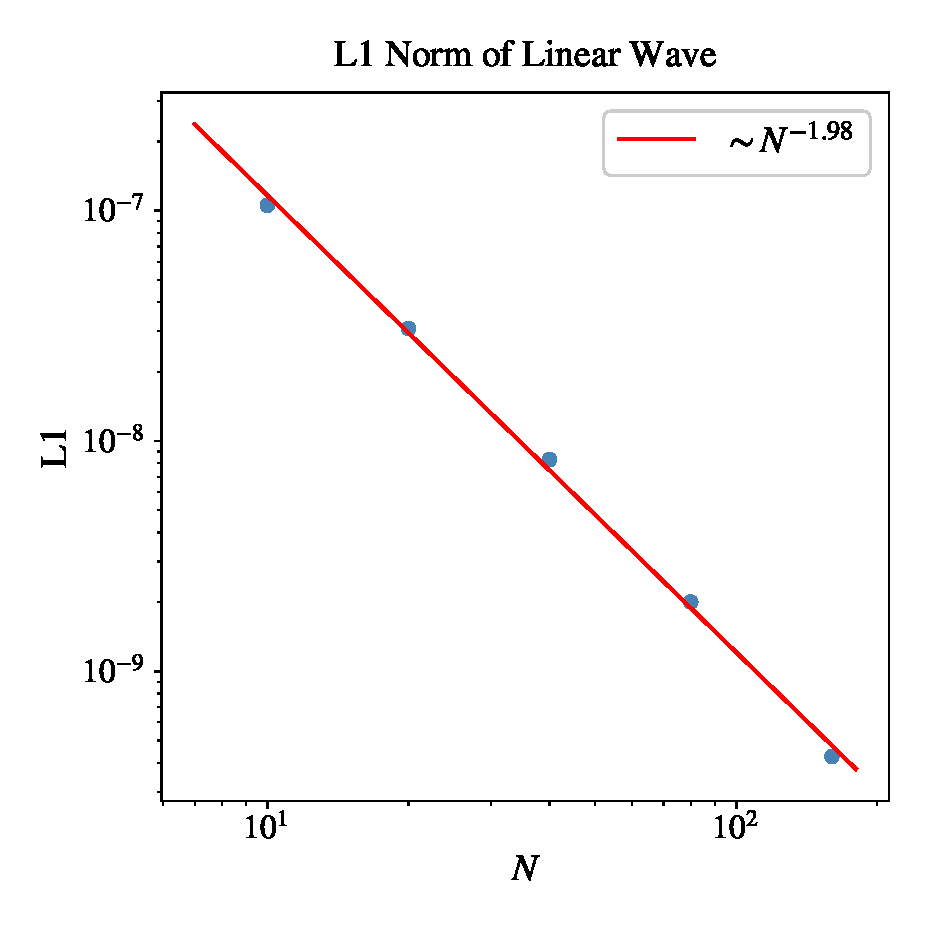
\includegraphics[width=0.4\textwidth]{figures/linear-wave-l1.eps}
        \caption{L1 norm of linear wave problem in 2d. Blue points are results
        of simulation from different resolutions overlaid by a linear fit showing
        the convergence is approximately second order. This example was produced by
        \textbf{linear\_wave\_2d.py} and \textbf{l1\_norm.py} scripts.}
        \label{fig.linear-wave}
    \end{center}
\end{figure}
Figure \ref{fig.linear-wave} shows the $L1$ norm as a function of grid cells per dimension.
As expected, the convergence rate is approximately second order in time and space for
this smooth problem. In the presence of shocks or other discontinuities it is not expected
to have such convergence.

\subsubsection{Sod shock-tube}
To examine the ability of the code to handle shock propagation we perform the Sod shock-tube 
problem \citep{toro-1997}. The problem consists of two different constant states at rest separated 
at the midpoint of the $x$ axis. A discontinuity exist in the density and pressure at that point. 
After $t=0$ the high density region flows into the lower density region. The flow produces a 
rarefaction, contact discontinuity, and a shock wave emanating from the density discontinuity. Thus, 
this problem creates a great test for the codes ability to capture the three wave types.

For our initial setup we use a unit box with reflective boundary conditions with density and pressure defined as
\begin{equation}
	\rho = \left\{
      \begin{array}{@{}ll@{}}
        	1.0 & \text{for}\ x \leq 0.5 \\
            0.125 & \text{for}\ x > 0.5
    	\end{array}\right.
\end{equation}
and
\begin{equation}
	P = \left\{
      \begin{array}{@{}ll@{}}
        	1.0 & \text{for}\ x \leq 0.5 \\
            0.1 & \text{for}\ x > 0.5
    	\end{array}\right.
\end{equation}
with $\gamma = 1.4$. The particles are laid out in a Cartesian grid and the simulation is evolved
until $t=0.15$. The number of particles per dimension is chosen to be $N=100$ and $N=45$ for 2D
and 3D respectively. This allows a comparison of a high and low resolution run.
\begin{figure}
    \begin{center}
        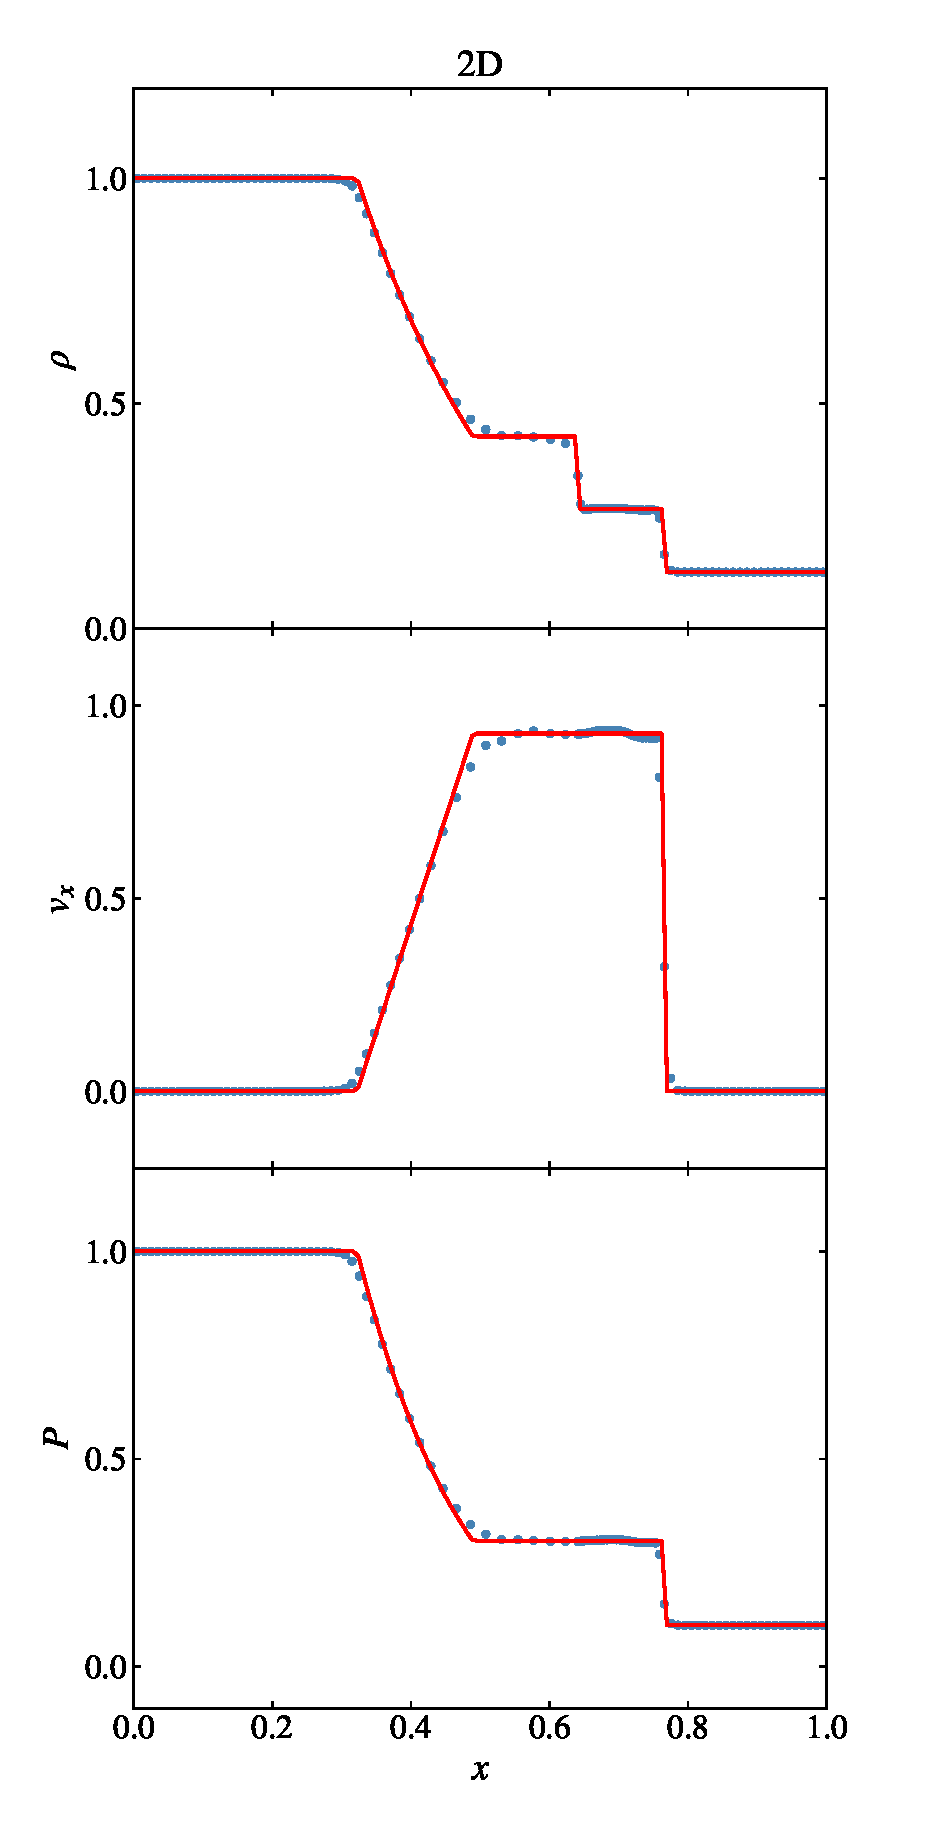
\includegraphics[width=0.4\textwidth]{figures/sod_2d.eps}
        \includegraphics[width=0.4\textwidth]{figures/sod_3d.eps}
        \caption{Profiles of density, $x$-component of velocity and pressure of the Sod 
        shock-tube simulation. Left: 2D run using a total of $100\times100$ particles. Right: 3D run 
        using a total of $45\times45\times45$, we only plot a slice of particles defined by $z=0$.
        Light blue points are the simulation while the red line is the exact solution.
        This example was produced by \textbf{sod\_2d\_cartesian.py},
        \textbf{sod\_3d\_cartesian.py}, \textbf{sod\_2d\_profiles.py}, and 
        \textbf{sod\_3d\_profiles.py} scripts.}
        \label{fig.sod}
    \end{center}
\end{figure}

Figure \ref{fig.sod} plots the particles density, $x$-component of velocity and pressure; only 
particles with $z=0$ are plotted in the 3D run for simplicity. The red line is the analytical 
solution. For the 2D simulation we can see the shock is well resolved as is the contact 
discontinuity. Further, the Lagrangian nature of the code can be seen as many particles have been 
squeezed between the contact discontinuity and the shock front while particles in the rarefaction 
have been spread out. For the 3D, lower resolution run, the code catches all three waves. Although, 
the contact discontinuity wave has been smoothed due to the lower number of particles.

\subsubsection{Explosion}
\begin{figure}
    \begin{center}
        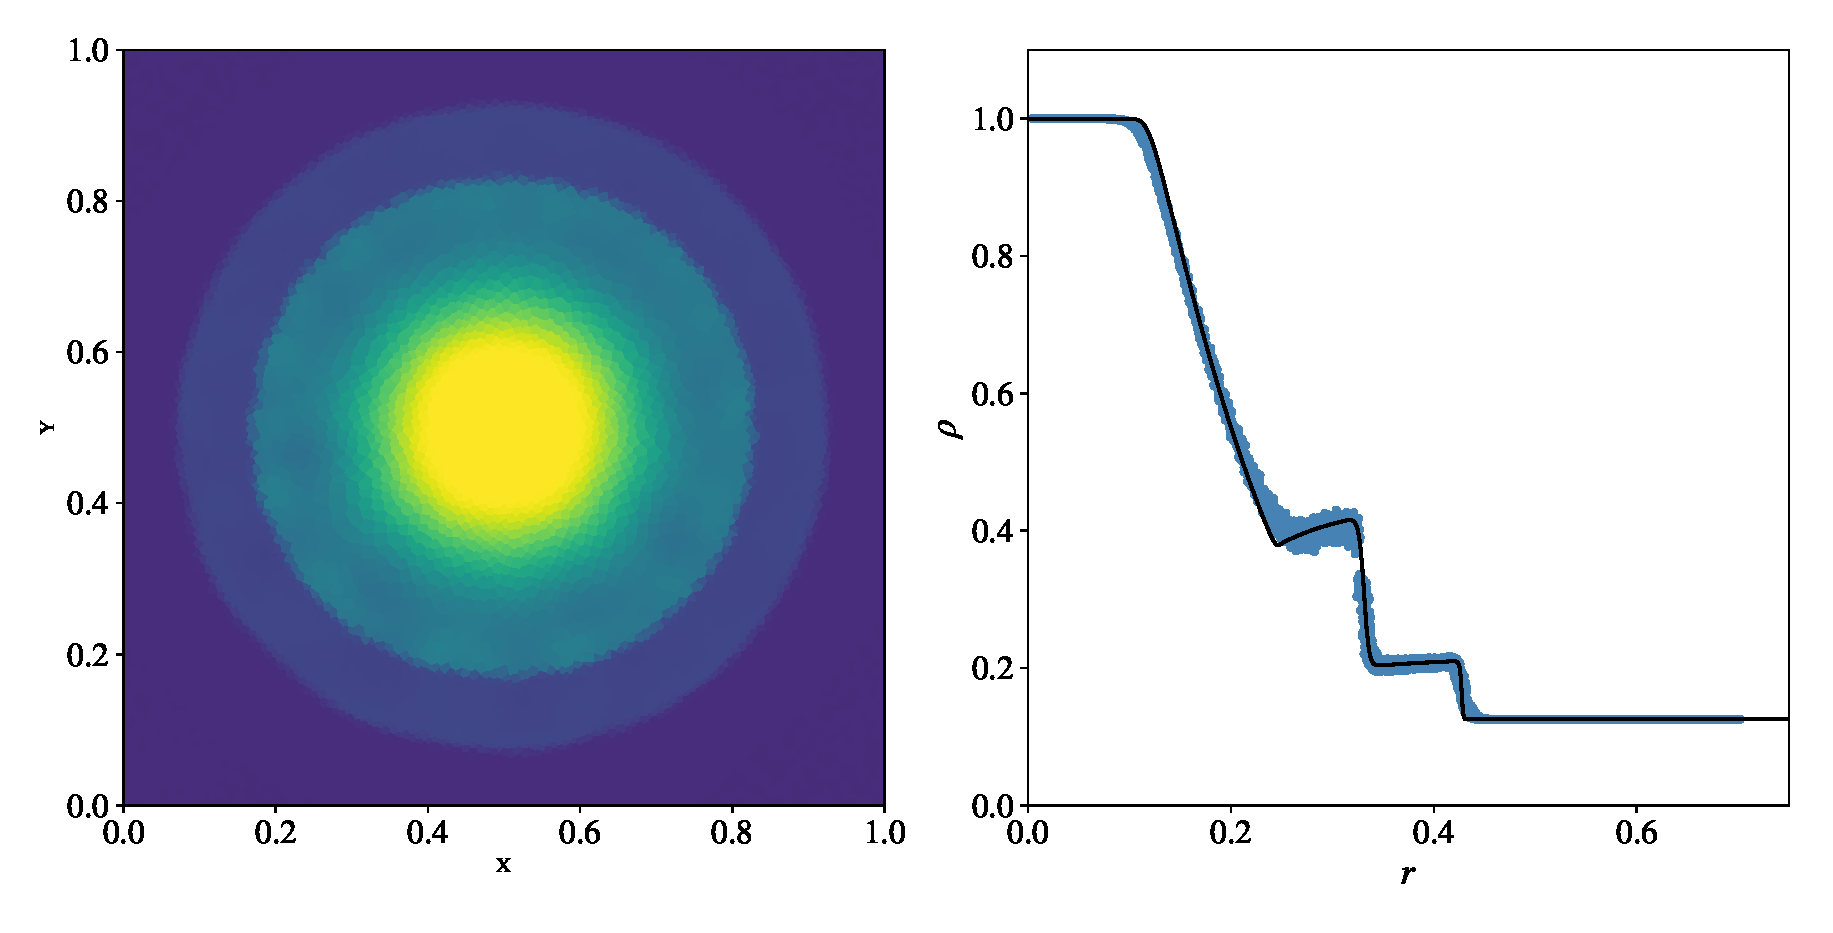
\includegraphics[width=0.8\textwidth]{figures/explosion_2d.eps}
        \caption{Density heatmap and radial profile of the Explosion problem. Left density
        heatmap, the irregular cells can been seen from the random initialization. Right
        radial density profile is an agreement with the exact solution in red.
        This example was produced by \textbf{explosion\_2d\_random.py} and 
        \textbf{explosion\_density\_panel.py} scripts.}
        \label{fig.explosion_2d}
    \end{center}
\end{figure}
An analog to the Sod problem is the 2D explosion problem \citep{toro-1997}. Like the Sod problem, 
the domain is partitioned into two constant states. However, the higher density region is now a 
circular region of radius $r$ centered in a unit box. Similar to the Sod problem, the initial 
conditions generate a shock, contact discontinuity and rarefaction wave. However, in this case
the waves are now a circular shock traveling radially outward, a circular contact
discontinuity traveling in the same direction, and a rarefaction wave traveling towards the
center.

We use the same values as the Sod problem except we restrict the higher density values onto
the center of domain with radius $r=0.25$. Further, instead of using a Cartesian grid we sample
particles uniformly for a unit square and perform 10 iterations of Lloyds algorithm. 

Figure \ref{fig.explosion_2d} shows the density map and density profile. Clearly, the cells
density matches the analytical solution in red. Further, the solution captures all three waves
even though the mesh was built in a random fashion. This an important difference over Eulerian
codes, since Lagrangian codes are not constrained to any initial particle placement. Therefore
one can reach better accuracy by placing the particles in way that exploits the problem. We will
see a later example of this in the Evrards problem, see Section \ref{sec.evrards}.

\subsubsection{Gresho vortex}
Our next problem will test stability of the code in maintaining equilibrium. \cite{Gresho90}, 
introduced an interesting problem to test for conservation of angular momentum. A vortex in a unit 
2D box with constant density $\rho=1$ is setup with the following angular velocity
\begin{equation}
	v_\phi (r) = \left\{
      \begin{array}{@{}ll@{}}
        	5r & \text{for}\ 0 \leq r < 0.2 \\
            2-5r & \text{for}\ 0.2 \leq r < 0.4 \\
            0 &\text{for}\ \geq 0.4
    	\end{array}\right.
\end{equation}
The angular velocity of the vortex grows linearly as one moves radially outward from
the center until midway of the disk. Then the velocity decreases linearly until it
vanishes at the rim of the disk. This produces triangular shape velocity profile.
The corresponding pressure is
\begin{equation}
	P(r) = \left\{
      \begin{array}{@{}ll@{}}
        	5 + 25/2r^2 & \text{for}\ 0 \leq r < 0.2 \\
            9+25/2r^2 - 20r + 4\ln(r/0.2) & \text{for}\ 0.2 \leq r < 0.4 \\
            3 + 4\ln(2) &\text{for}\ \geq 0.4.
    	\end{array}\right.
\end{equation}
The pressure is chosen such that the pressure gradients balance the centrifugal forces
generated by the rotation. Thus producing a solution that is independent of time.
\begin{figure}
    \begin{center}
        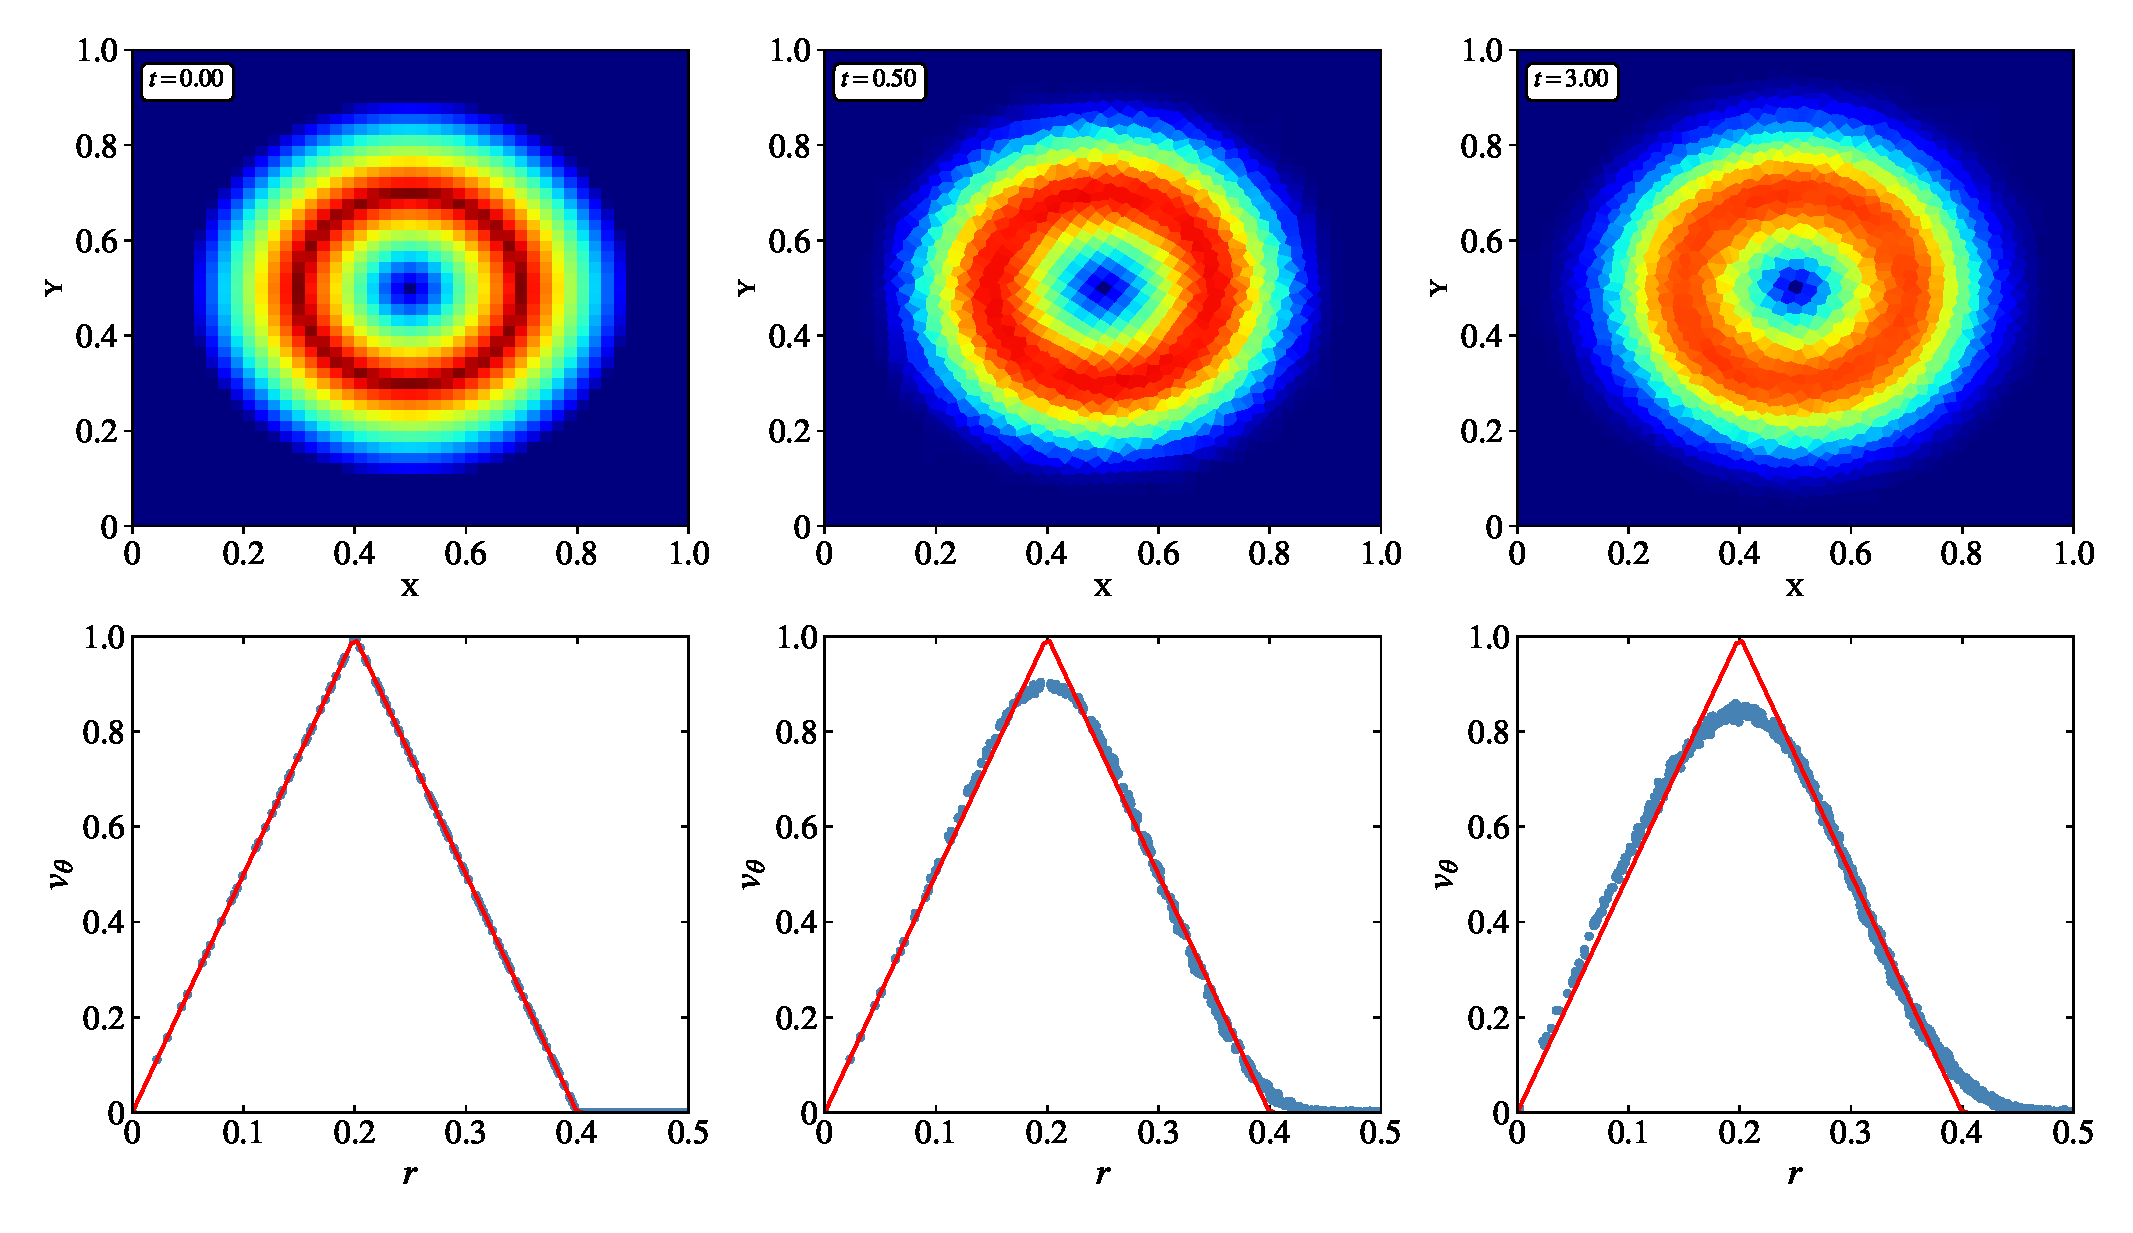
\includegraphics[width=0.8\textwidth]{figures/gresho_vortex.eps}
        \caption{Heatmap and radial profile of azimuthal velocity. Top row: time evolution
        of the cells at times $t=0.0, 0.5, 3.0$. Bottom row: corresponding radial profile of 	
        azimuthal velocity. As the simulation evolves the systems remains in equilibrium.
        This example was produced by \textbf{gresho\_2d\_cartesian.py} and 
        \textbf{gresho\_density\_panel.py} scripts.}
        \label{fig.gresho_vortex}
    \end{center}
\end{figure}
Figure \ref{fig.gresho_vortex} shows three snapshots at $t=0.0, 0.5, 3.0$ of the azimuthal
velocity. The top row is a 2d heat map while the bottom row is a radial profile. At time $t=0$
all the cells are rectangular. As the system evolves the cells that are rotating become irregular 
polygons. There is a small amount of velocity smoothing at the initial largest velocities and at
the rim of the vortex. However, it is evident that the system stays in equilibrium.

\subsubsection{Sedov-Taylor}
Another test that generates a shock is the Sedov-Taylor blast wave problem \citep{Sedov1959}. In 
this problem a homogeneous gas is injected with a large amount of energy in a point-like region at 
the center of the domain. A spherical shock is created emanating from the center. The shock 
propagates radially outward sweeping mass into a thin shell and creating a cavity behind the shock. 
The problem has a well known analytical self-similar solution; see \cite{Sedov1959} for details. 
Applying the Rankine–Hugoniot at the shock front the density jumps to a maximum compression of
\begin{equation}
	\rho_{\mathrm{max}}/\rho = (\gamma + 1)/(\gamma - 1),
\end{equation}
for $\gamma = 5/3$ this amounts to a max value of 4.

We consider the 2D and 3D case. A unit box is setup with particles in a Cartesian grid of size
$45\times 45$ and $45 \times 45 \times 45$ for 2D and 3D respectively. The stationary gas has
a constant density of $\rho = 1.0$ and pressure $P = 10^{-6}$ with $\gamma=5/3$. The simulation is
allowed to evolve to time $t=0.06$.
\begin{figure}
    \begin{center}
        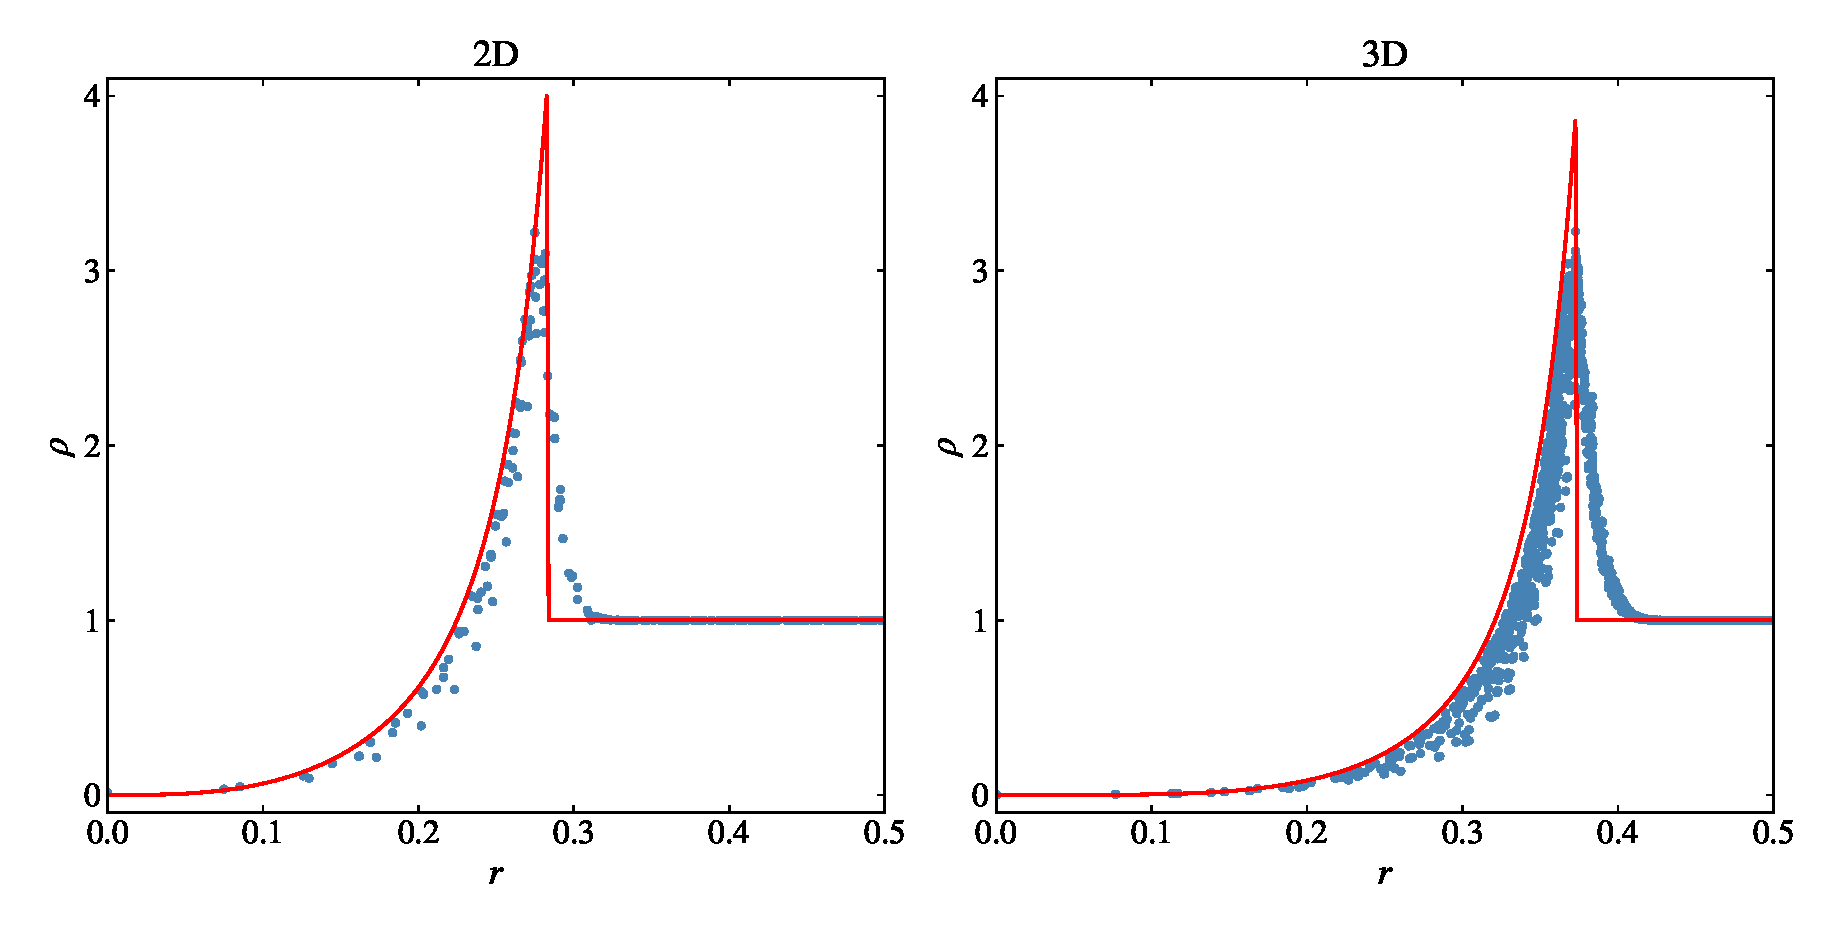
\includegraphics[width=0.8\textwidth]{figures/sedov_compare.eps}
        \caption{Density profile of Sedov-Taylor blast wave problem. Left: 2D version with an 
        initially Cartesian mesh of $45 \times 45$. Right: 3D version with an initially 
        Cartesian mesh of $45 \times 45 \times 45$; only a random sample of $45\times45$ is
        plotted for simplicity. Light blue points are the density at radius $r$ 
        from the center of the explosion while the red line is the exact solution.
        This example was produced by \textbf{sedov\_2d\_cartesian.py},
        \textbf{sedov\_3d\_cartesian.py}, and \textbf{sedov\_density\_compare.py} scripts.}
        \label{fig.sedov}
    \end{center}
\end{figure}
Figure \ref{fig.sedov} shows the cell density as a function of radial distance from the center of 
the explosion. It is noted that shock is well resolved by the cells as the mesh has deformed in such 
a way that the shock front contains a large amount of cells which is evident in
Figure \ref{fig.sedov_panel}.
\begin{figure}
    \begin{center}
        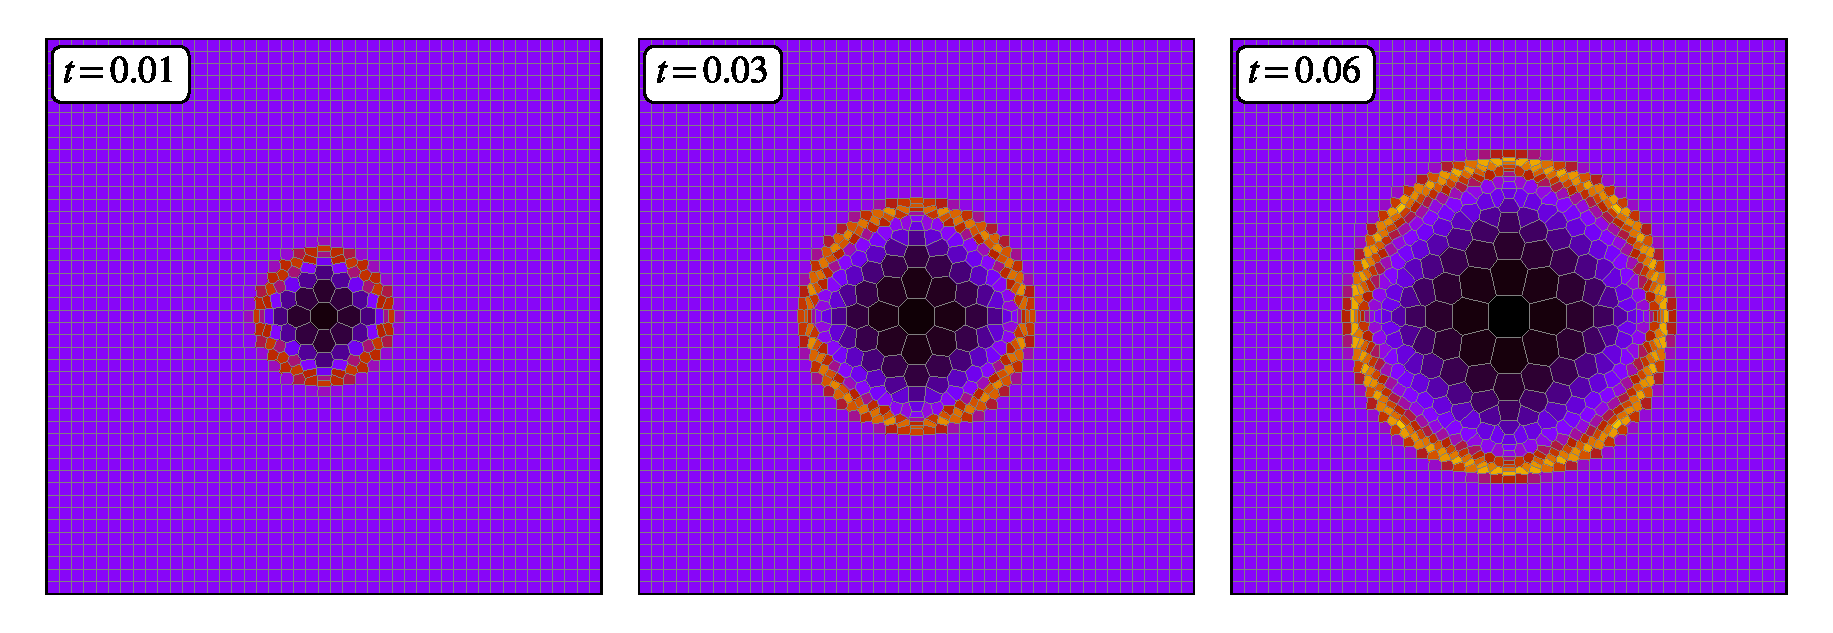
\includegraphics[width=0.8\textwidth]{figures/sedov_panel.eps}
        \caption{Evolution of the density at several times. The initial cell with the energy
        imparted remains stationary as the cells around it move radially outward. The cells at
        the shock are compressed allowing for better resolution. This example was produced by 
        \textbf{sedov\_2d\_cartesian.py} and \textbf{sedov\_density\_panel.py} scripts.}
        \label{fig.sedov_panel}
    \end{center}
\end{figure}
The center cell, where the energy is deposited, remains stationary while the
cells around it move radially outward. The cells exterior to the shock remain
stationary until they are swept and compressed by the shock.

\subsubsection{Kelvin-Helmholtz instability}
For our last hydrodynamic test we consider the Kelvin-Helmholtz (KH) instability. This
problem consist of a shear-flow where a single mode is excited by a velocity perturbation.
Specifically, two layers with different densities are initially in pressure equilibrium. 
Each layer flows in the opposing direction and receives a velocity perturbation perpendicular
to the interface. The perturbation grows exponentially and produces structures which
are called KH instabilities. A difficulty of this problem is that
numerical errors, noise, and resolution seed spurious small structure \citep{Lecoanet2016}
making direct comparisons a difficult endeavor. However, we can use this problem to
visually verify the characteristics of the problem are maintained
and leave the exact detail treatment to the next revision of the code.

We follow \cite{Springel2010} and setup a unit periodic box with density
\begin{equation}
	\rho = \left\{
      \begin{array}{@{}ll@{}}
            2 & \text{for}\ y < 0.25 \\
            1 & \text{for}\ 0.25 \leq y \leq 0.75\\
            2 & \text{for}\ 0.75 < y,
    	\end{array}\right.
\end{equation}
$x$-component of velocity
\begin{equation}
	v_x = \left\{
      \begin{array}{@{}ll@{}}
            -0.5 & \text{for}\ y < 0.25 \\
            0.5 & \text{for}\ 0.25 \leq y \leq 0.75\\
            -0.5 & \text{for}\ 0.75 < y,
    	\end{array}\right.
\end{equation}
and $y$-component of velocity
\begin{equation}
	v_y(x, y) = w_0 \mathrm{sin}(4\pi x) \left(\exp\left(-\frac{(y-0.25)^2}{2\sigma^2}\right) +
    	\exp\left(-\frac{(y-0.75)^2}{2\sigma^2}\right)\right)
\end{equation}
where $w_0=0.1$ and $\sigma=0.05/\sqrt{2}$. The pressure is set to $P=2.5$, $\gamma=5/3$
and the simulation is evolved until time $t=2$.
\begin{figure}
    \begin{center}
        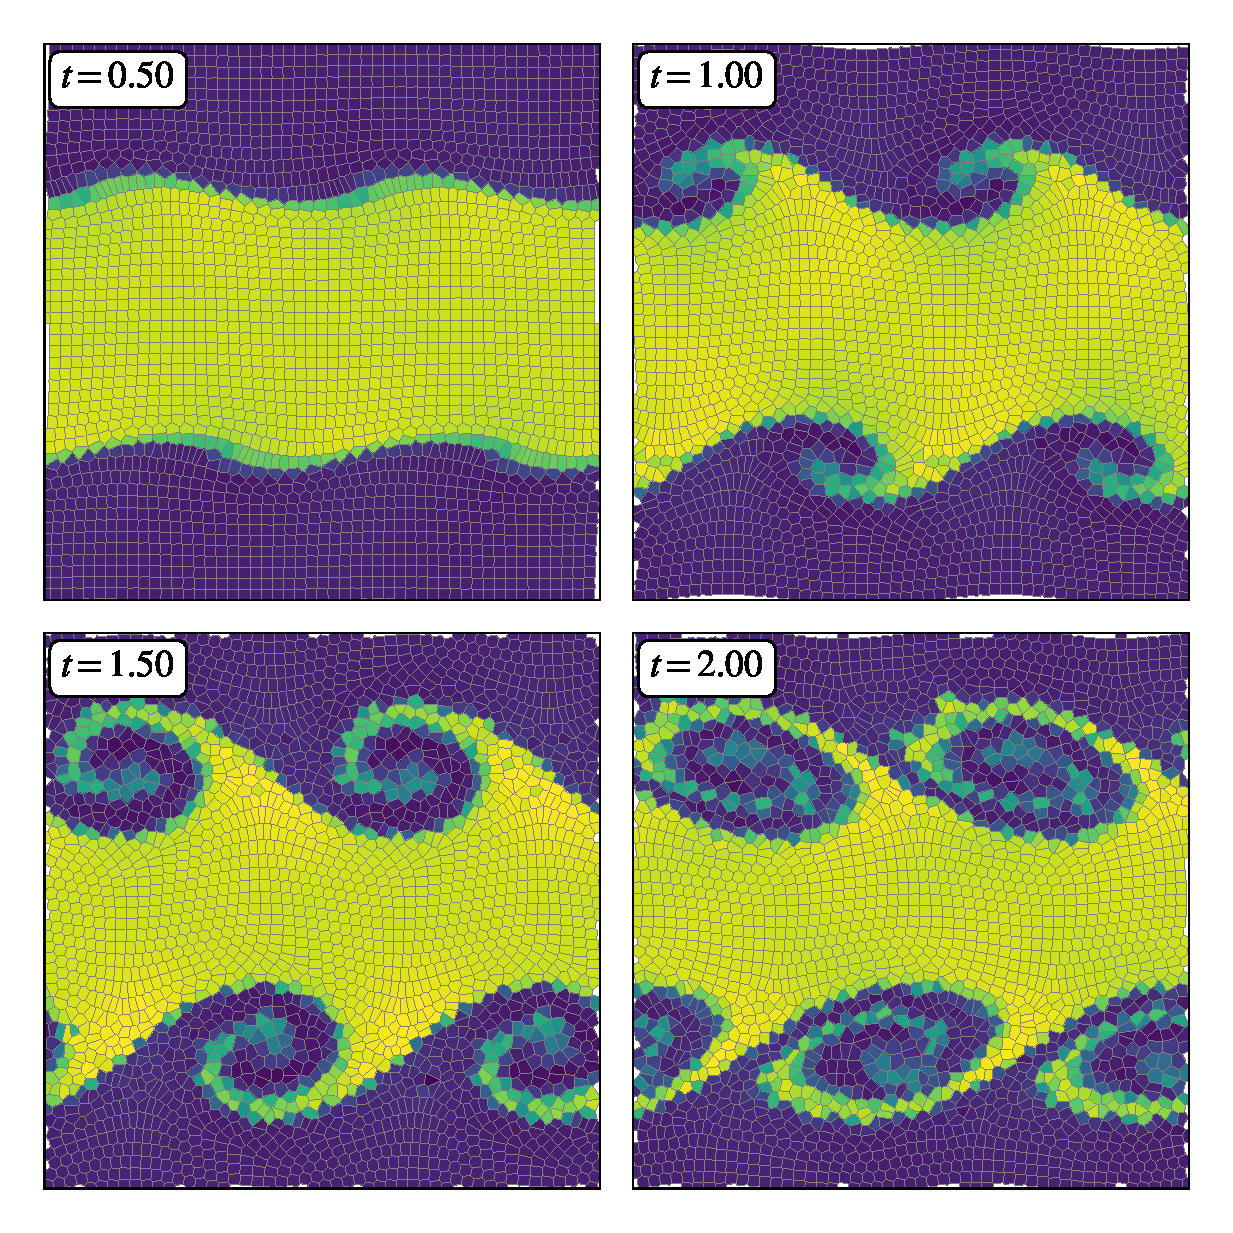
\includegraphics[width=0.8\textwidth]{figures/kelvin.eps}
        \caption{Evolution of the density at several times in the KH problem. We see the common
        traits of KH evolution, KH billows and mixing. This example was produced by 
        \textbf{kelvin\_helmholtz\_2d\_cartesian.py} and 
        \textbf{kelvin\_helmholtz\_density\_panel.py} 
        scripts.}
        \label{fig.kelvin}
    \end{center}
\end{figure}

Figure \ref{fig.kelvin} shows the density field for several selected times. Comparing with
Springel, visually we conclude that the results are in close agreement. The formation of the
Kevlin Helmholtz billows and mixing of both fluids at each time are similar.

\subsection{Gravity Tests}
\subsubsection{Two body}
Our first problem, in testing our gravity solver, is a simple two body problem where two particles
interact with each other through their gravitational force. Although, this problem does not really test the 
implementation of the gravity tree, since only two leaves will be constructed
in the tree and it is most likely that the leaves will interact with each other bypassing the node 
moments, it does test the gravity kernel and stability of the leap frog integrator.

For this problem an exact solution exists by reducing it to a single body. Given
two particles with masses $m_1$ and $m_2$ with positions $\vec{r}_1$ and $\vec{r}_2$ the equation of motion for
the reduced mass
\begin{equation}
	\frac{1}{\mu} = \frac{1}{m_1} + \frac{1}{m_2}
\end{equation}
is
\begin{equation}
	\mu\frac{d^2 \vec{r}}{dt^2} = -\frac{G m_1 m_2}{r^2}\hat{r},
    \label{eq.reduced-force}
\end{equation}
where $\vec{r}$ is the separation vector $\vec{r}_1 - \vec{r}_2$. Equation \ref{eq.reduced-force} can be
transformed to polar coordinates giving the solution
\begin{equation}
	r = \frac{a(1-\epsilon^2)}{1-\epsilon cos(\theta)}
\end{equation}
for initial conditions $a$ and $\epsilon$. The overall system evolves with a period of
\begin{equation}
    T = \sqrt{\frac{4\pi^2 a^3}{G m}},
\end{equation}
where $m=m_1 + m_2$. To recover the particles positions, a final transformation
of the form
\begin{equation}
	\begin{array}{rcl}
		\vec{r}_1 & = & \frac{m_1}{m}\vec{r}\\
    	\vec{r}_2 & = & -\frac{m_2}{m}\vec{r}
    \end{array}
\end{equation}
is used. The initial position and velocity of the particles can be parameterized by $a$,
$\epsilon$ and $q=m_1/m_2$
\begin{equation}
	\begin{array}{rcl}
    	\vec{r}_1 & = & a\frac{1-\epsilon}{1+q} \hat{x}\\
        \vec{v}_1 & = & \frac{1}{1+q}\sqrt{\frac{1+\epsilon}{1-\epsilon}}\sqrt{\frac{Gm}{a}} \hat{y}\\
        \vec{r}_2 & = & -q \vec{r}_1\\
        \vec{v}_2 & = & -q \vec{v}_1.
    \end{array}
\end{equation}

We setup the particles with parameter values $a=0.5$ and $\epsilon=0.25/0.75$ with $G=1$ and allow
the simulation to evolve for 10 periods. The time step is held fixed with a value of $dt=T/1000$.
In Figure \ref{fig.two_body} we show the trajectory for both particles as well as the evolution of
the relative total energy error. We clearly see that both trajectories remain along the exact solution
signifying the stability of the leap frog integrator. Further we see that the relative total energy
error remains bounded by zero and $-1.1\times10^{-4}$ indicating that the total energy remains
accurately conserved.
\begin{figure}
    \begin{center}
        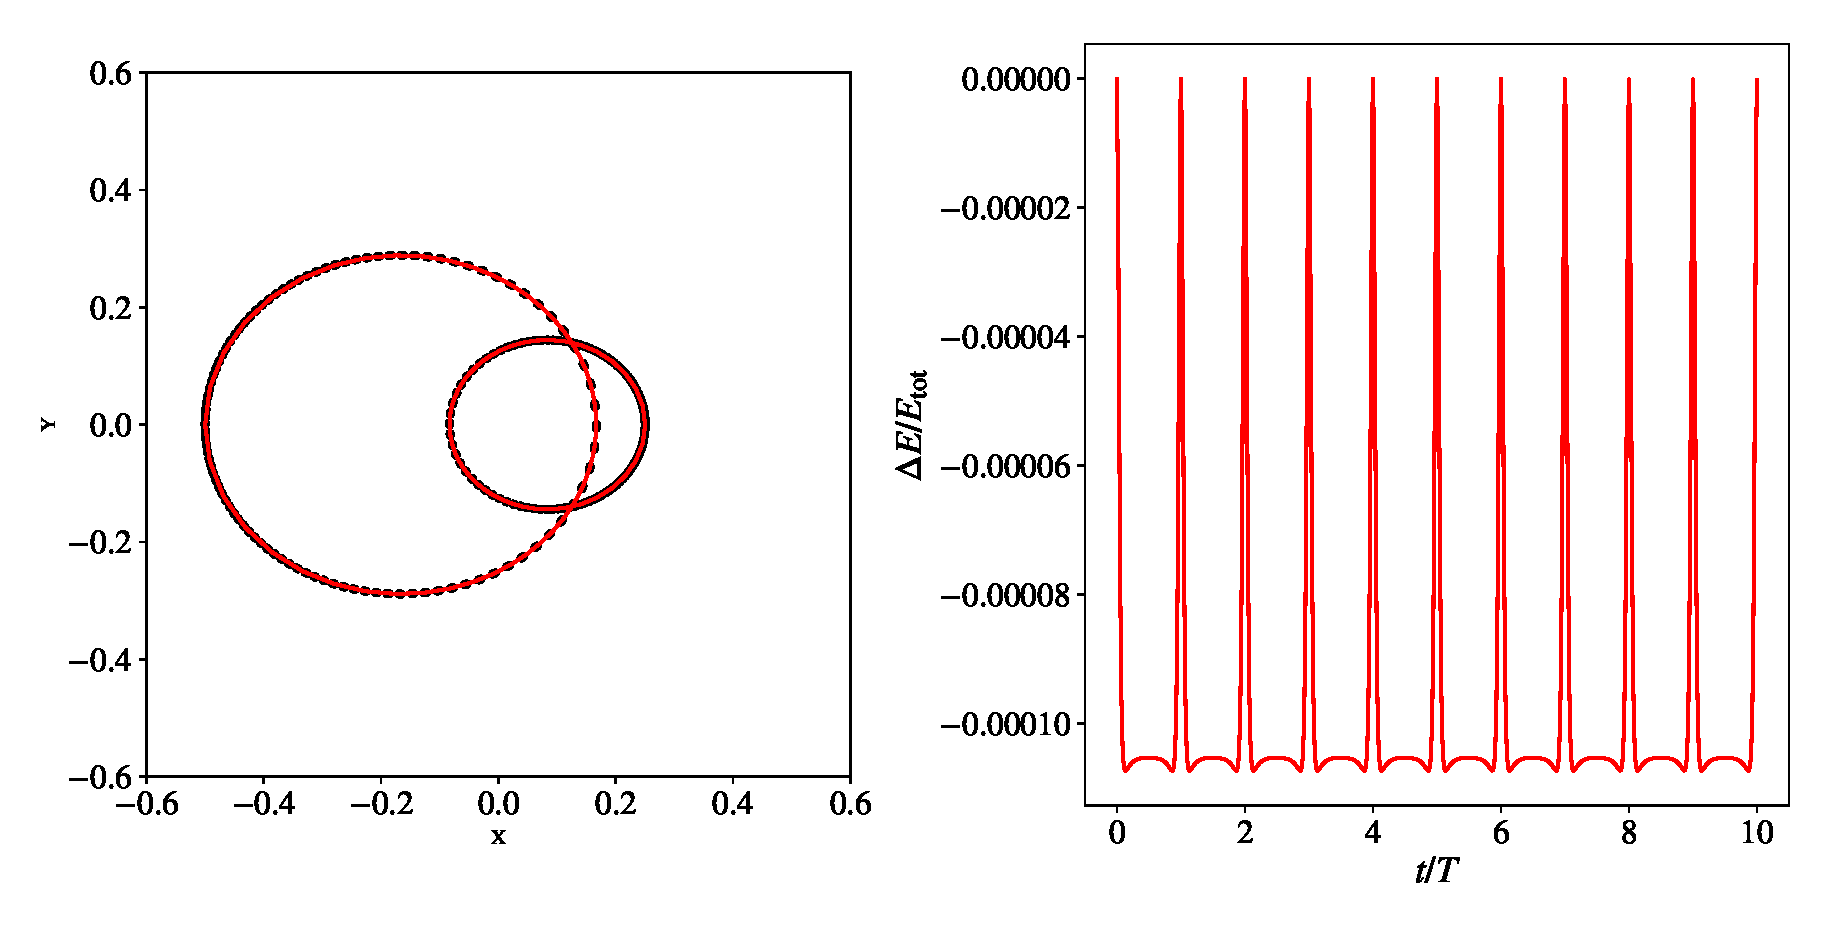
\includegraphics[width=0.9\textwidth]{figures/two_body.eps}
        \caption{Left: Trajectories of the two body problem for ten periods. Clearly
        both particles remain in their orbital path shown in red signifying the stability
        of the leap frog integrator. Right: Corresponding relative total energy error.
        The total energy remains accurately conserved as the worst relative error is
        $-1.1\times10^{4}$.}
        \label{fig.two_body}
    \end{center}
\end{figure}

\subsubsection{Plummer sphere}
The Plummer sphere cite is a model that can be used to describe the distribution of stars and in a cluster
and is commonly used to test gravity solvers. The Plummer sphere, i.e. a polytrope of index 5,
has a density profile of the from
\begin{equation}
	\rho (r) = \frac{3 M}{4\pi R^3} \left(1 + (r/R)^2\right)^{-5/2},
    \label{eq.plummer}
\end{equation}
where $M$ is the total mass of the cluster and $R$ is a scale parameter which sets the
size of the cluster. The system is in steady state with an isotropic velocity distribution.
To test our gravity solver, we initialize our particles with the given distributions and
advance the system in time. We expect the system to stay in steady state therefore we compare
the initial density distribution with the final state of the system.

For our test we chose the parameters of the Plummer sphere to be $M=1,000$ and $R=1$ with
$G=1$. We then sampled 10,000 particles using the the rejection technique outlined in
cite to set the position and velocities. The system is allowed to evolve to time $t=1$
which is roughly ten dynamical times. The gravitational tree used an opening angle 0.4
and smoothing parameter of 0.03.
\begin{figure}
    \begin{center}
        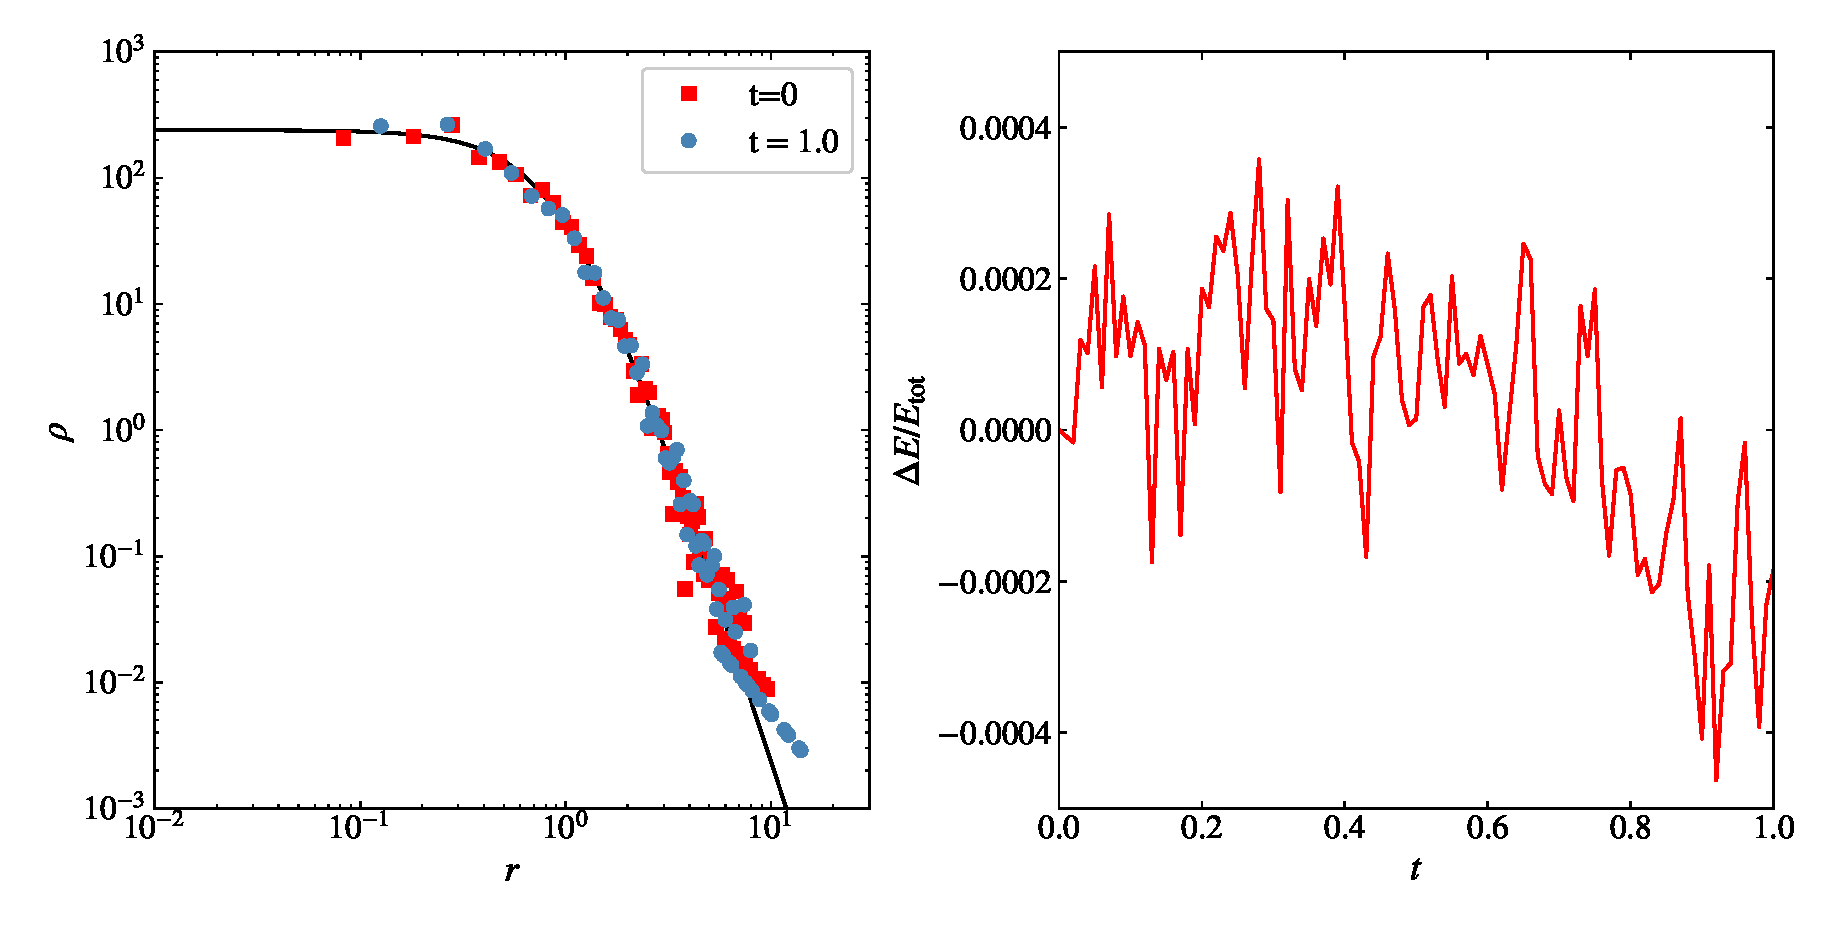
\includegraphics[width=0.9\textwidth]{figures/plummer.eps}
        \caption{Density profile of Sedov-Taylor blast wave problem. Left is the 2D version with an initially
        Cartesian mesh of $45 \times 45$. Right is the 3D version with an initially Cartesian mesh of 
        $45 \times 45 \times 45$. Light blue points are the density a radius $r$ from the center of the explosion
        while the red line is the exact solution.}
        \label{fig.plummer}
    \end{center}
\end{figure}
The left panel of Figure \ref{fig.plummer} shows the density profile at the initial and final 
time of the simulation with equation \ref{eq.plummer} overlaid as a reference. The density is calculated
by dividing the space by spherical shells, binning and dividing by the volume. It is clearly shown that
at the final time the particles remain in steady state with their positions matching the initial
distribution. The right panel of \ref{fig.plummer} shows the evolution of the relative error of the
total energy of the system. The error stays well below $5\times 10^{-4}$ with a final error of
$2\times 10^{-4}$, entailing the solver has accurately maintained the total energy.

\subsubsection{Rayleigh Taylor}
Our first hydrodynamic problem to include gravity is the Rayleigh Taylor instability problem.
The problem consists of dense fluid over a lighter fluid in the presence of a uniform 
vertical gravitational field. A perturbation is placed in the vertical direction causing the
dense field to sink while the lighter rises through buoyancy.

A rectangular domain of the size $[1\times3]$ is chosen with the gravitational force in the
$y$-direction with strength of $g=1$. The initial setup of the density
is
\begin{equation}
	\rho = \left\{
      \begin{array}{@{}ll@{}}
            1 & \text{for}\ y \leq 1.5 \\
            2 & \text{for}\ 5 > 1.5,
    	\end{array}\right.
\end{equation}
while the pressure is
\begin{equation}
	P = \left\{
      \begin{array}{@{}ll@{}}
            10 - y & \text{for}\ y \leq 1.5 \\
            11.5 + 2(y-1.5) & \text{for}\ 5 > 1.5,
    	\end{array}\right.
\end{equation}
such that the system is initially in hydrostatic equilibrium. A perturbation is applied
to the $y$-velocity
\begin{equation}
	v_y = \mathrm{cos}\left(2\pi x\right)\exp{-(y-1.5)^2/0.1}
\end{equation}
We set $\gamma=1$ and let the system evolve to $t=3.0$. Although without an implementation
of viscosity there is no one correct solution that all codes converge to. However, we can
visually inspect if our simulation share the same characteristics of another established
code. In Figure we that the single mode is very similar to the results from cite
\begin{figure}
    \begin{center}
        \includegraphics[width=0.6\textwidth]{figures/rayleigh_compare.eps}
        \caption{Density profile of Sedov-Taylor blast wave problem. Left is the 2D version with an initially
        Cartesian mesh of $45 \times 45$. Right is the 3D version with an initially Cartesian mesh of 
        $45 \times 45 \times 45$. Light blue points are the density a radius $r$ from the center of the explosion
        while the red line is the exact solution.}
        \label{fig.rayleigh}
    \end{center}
\end{figure}

We see the mode has the characteristics of

\subsubsection{Evrard Collapse}
\label{sec.evrards}
The final test is the Evrards collapse problem which tests the coupling of self-gravity and hydrodynamics.
The problem consists of an initially non-rotating isothermal gas sphere with mass $M=1$ and radius $R=1$
with a density 
\begin{equation}
	\rho(r) = \left\{
      \begin{array}{@{}ll@{}}
            1/\left(2\pi r\right) & \text{for}\ r \leq 1 \\
            0 & \text{for}\ r > 1
    	\end{array}\right.
\end{equation}
and pressure
\begin{equation}
	P(r) = \left\{
      \begin{array}{@{}ll@{}}
            0.05 /\left(3\pi r\right) & \text{for}\ r \leq 1 \\
            0 & \text{for}\ r > 1.
    	\end{array}\right.
\end{equation}
The gravitational constant is set to $G=1$ and $\gamma=5/3$. The evolution of the sphere begins
with mass falling towards the center due to self-gravity. The pressure at the center rises and
produces a shock traveling outward through the in-falling gas. The final state of the gas is a
spherical distribution in hydrostatic virial equilibrium.

We setup an initial Cartesian grid of size $33\times 33\times 33$ particles. Due to the nature
of the $1/r$ density profile, a Cartesian mesh will not resolve the high density values unless
the resolution is sufficiently increased. However we have complete freedom on how to the particles
are initially setup. Therefore, we transform particles radially inside the sphere by the following
\begin{equation}
    r_{\mathrm{new}} = r_{\mathrm{old}}^{3/2}.
\end{equation}
Such a transformation maps a grid of equally spaced particles with uniform density to
a set of particles spaced in such a way that the uniform density follows a $1/r$ profile. 
\begin{figure}
    \begin{center}
        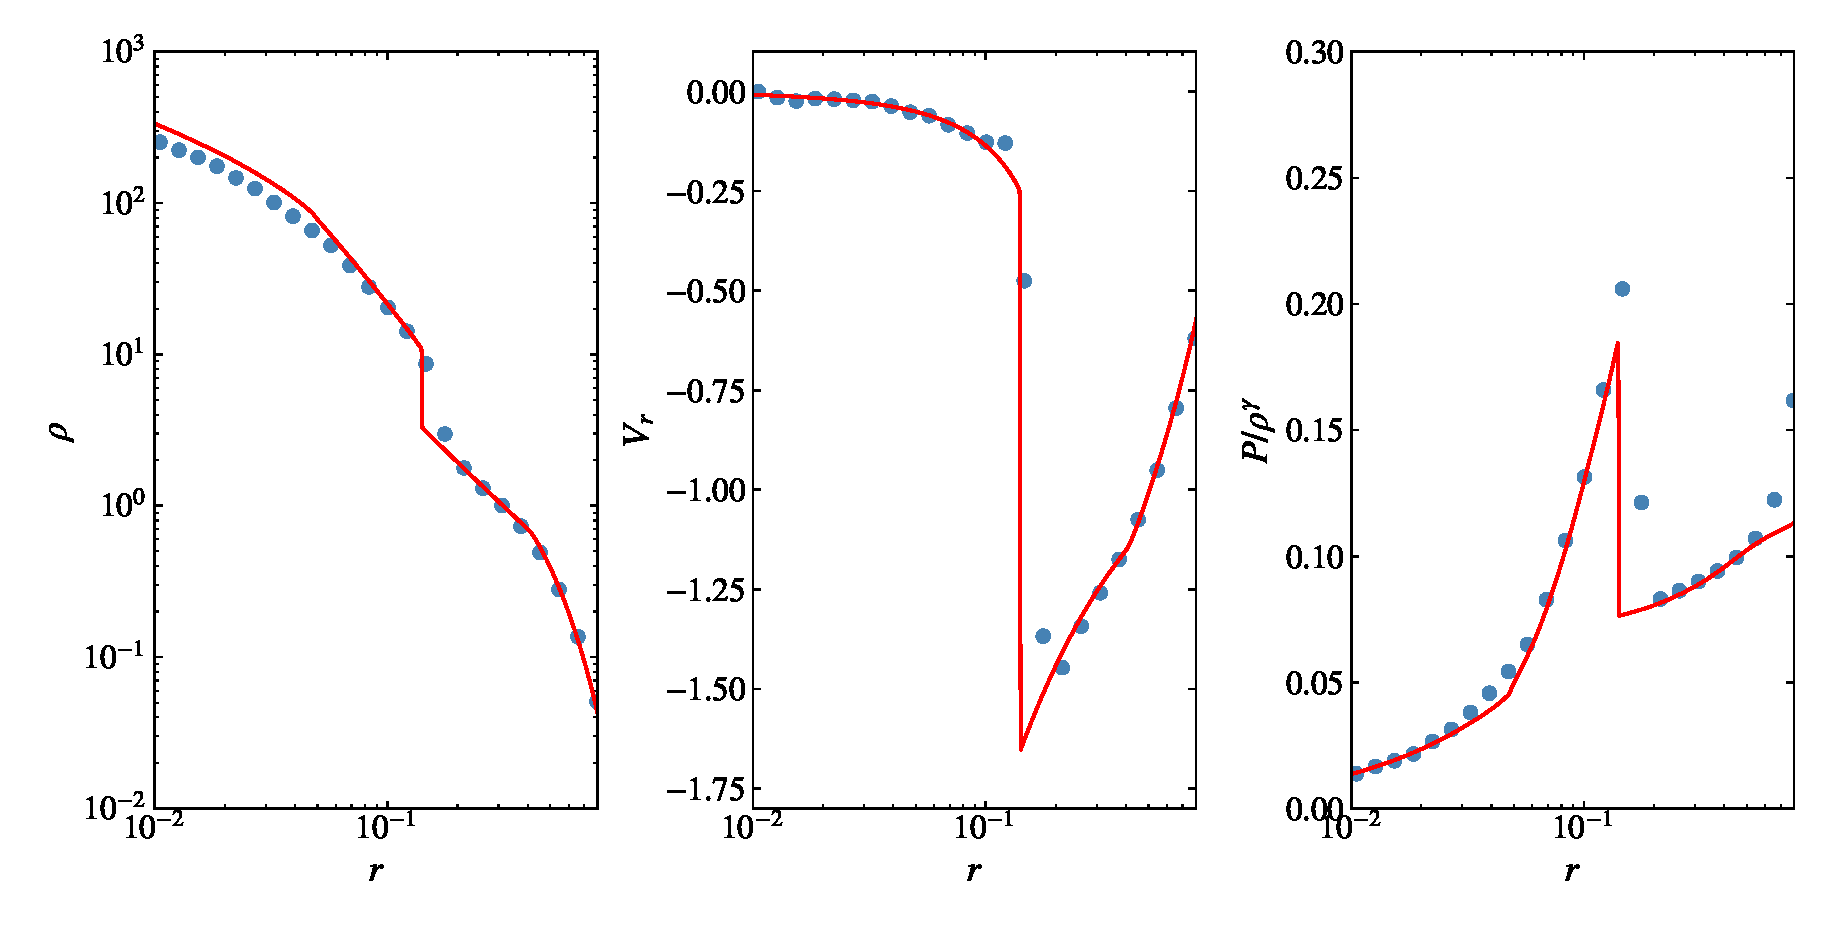
\includegraphics[width=0.9\textwidth]{figures/evrard.eps}
        \caption{Density profile of Sedov-Taylor blast wave problem. Left is the 2D version with an initially
        Cartesian mesh of $45 \times 45$. Right is the 3D version with an initially Cartesian mesh of 
        $45 \times 45 \times 45$. Light blue points are the density a radius $r$ from the center of the explosion
        while the red line is the exact solution.}
        \label{fig.evrard}
    \end{center}
\end{figure}

The radial averaged density, radial velocity and entropy are shown in Figure at time $t=0.81$
when the shock has formed and is traveling outward. We see all profiles adequately follow the
exact solution in red for this low resolution run. Further we see that there is significant
error in the conservation of energy Figure. This is expected as noted by Springel. The 
discrepancy arises from the gravitational work term which ignores the motion of mass
exchanged by adjacent cells. Springel proposed a new formulation for then energy equation
that results in better energy conservation. This updated method will be added in the next
revision of the code.
\begin{figure}
    \begin{center}
        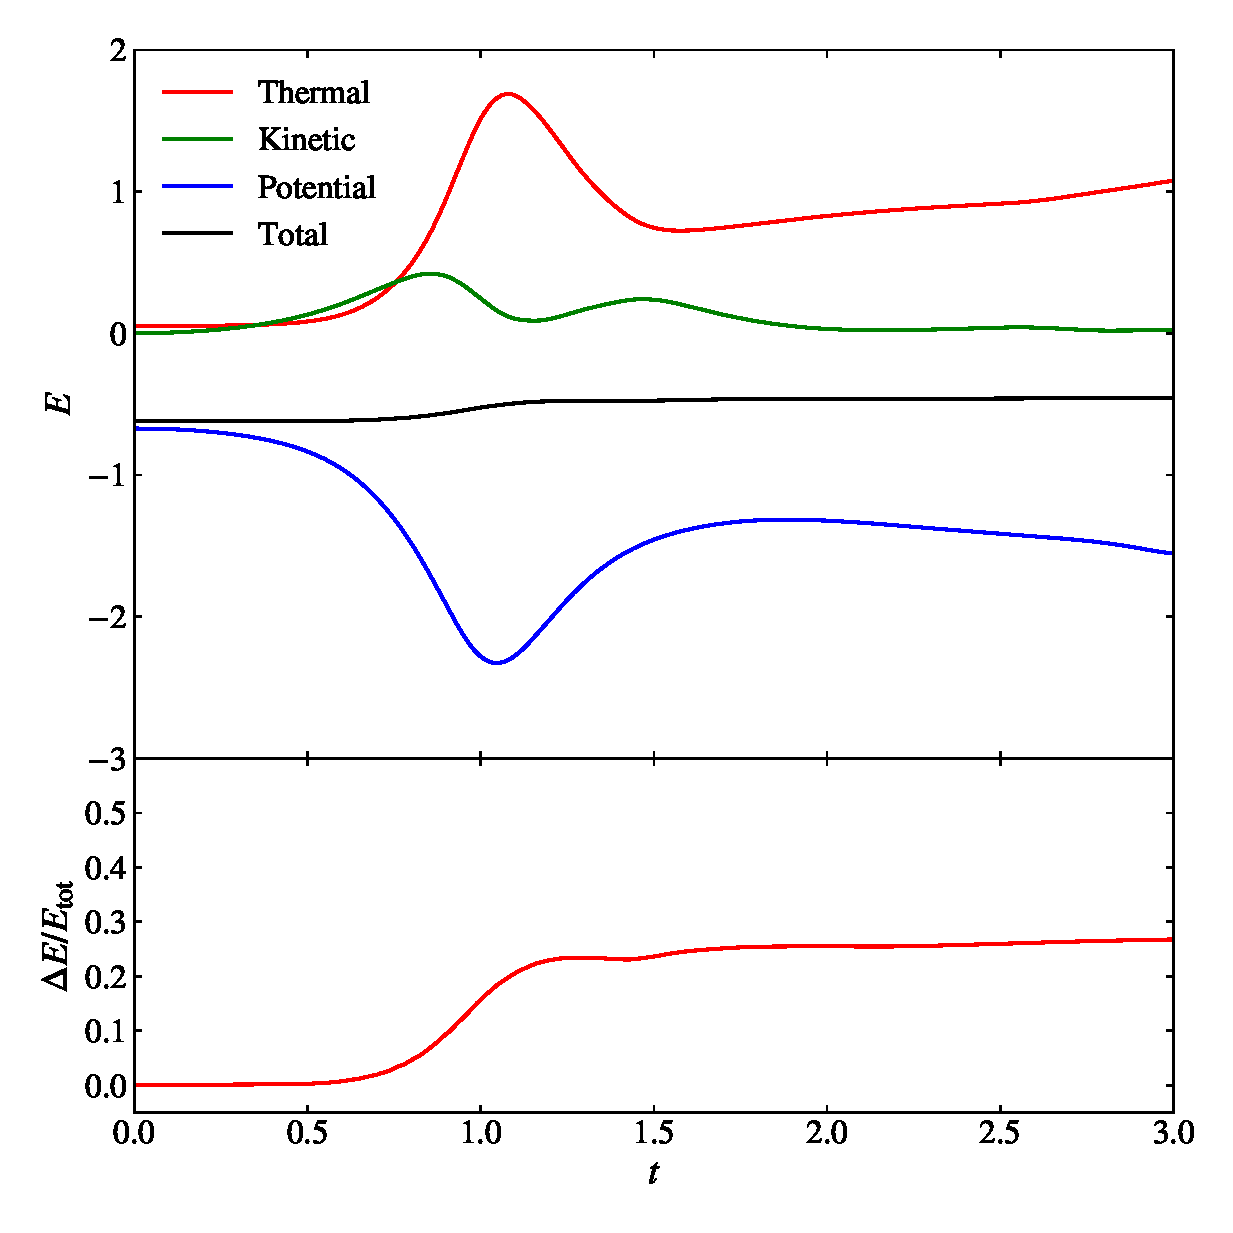
\includegraphics[width=0.6\textwidth]{figures/evrard_energy.eps}
        \caption{Density profile of Sedov-Taylor blast wave problem. Left is the 2D version with an initially
        Cartesian mesh of $45 \times 45$. Right is the 3D version with an initially Cartesian mesh of 
        $45 \times 45 \times 45$. Light blue points are the density a radius $r$ from the center of the explosion
        while the red line is the exact solution.}
        \label{fig.evrard_energy}
    \end{center}
\end{figure}

%
%%% Section: parallelism and performance
%\section{Parallel Strategy and Performance}
\label{sec.parallel}

\subsection{Parallel Strategy}

The current version of \enzo\ has been parallelized for distributed
memory platforms using the Message Passing Interface (MPI).  This is
done using a single grid object as the basic unit of parallelization.
Each grid object -- including all cell and grid data -- is fully
contained on a single processor\footnote{In this context, we use the
word {\it processor} to mean a basic distribution unit; this could be
either a core or a node, depending on details of the system.  Note
that the current version of \enzo\ is not threaded, although a hybrid
MPI + OpenMP version is under development.}.  Parallelization is
accomplished by distributing grids amongst processors.  This is done
on the root grid using a simple tiling system, where the root grid is
split up into $N_{\rm root}$ tiles, with $N_{\rm root}$ typically
equal to the number of processors, $N_p$.

Load balancing on levels other than the root level (i.e., grids for
which the level $l > 0$) is different, as the refined patches are not
generally uniformly distributed.  Grids on refined levels are first
placed on the same processor as their parent to minimize
communication; however, this generally does not result in a
well-balanced computational load.  Therefore, the code has a number of
options for load balancing the grids on a given level. Each grid is
assigned an estimated computational load, generally equal to the
number of cells in the grid (which, empirically, is a good estimate of
computational cost).  The first load-balancing option is to move a
grid from the processor with the highest computational load to the
processor with the lowest load, with the proviso that only grids with
load factors less than half the difference between the highest and
lowest loaded processors will be moved.  This continues until the load
ratio between the most-to-least loaded processor is below 1.05 or
until no suitable grid can be found to transfer.  A second load
balancing option uses a space-filling Hilbert curve to order the grids
by their approximate spatial position.  Then, once the grids have a
specific one-dimensional ordering, we can divide up the grids into
$N_p$ groups (with the division taking place as equally as possible).
Load balancing is done separately for each level.  Clearly load
balancing is most successful if there are significantly more grids
than processors; however, small grids are less efficient because of
the large number of ghost zones compared to active zones, and so the
code uses a simple heuristic in order to split up grids until there
are of order 10 grids per processor.  This generally results in good
load-balancing while not producing grids that are wastefully small.

Communication between processors is done using a non-blocking
communication strategy that allows overlap of communication and
computation.  This can be done efficiently because each processor
retains a copy of the entire hierarchy of grids, except that grids
that do not `live' on a given processor only contain meta data
(essentially just the location and size of the grid; such grids are
denoted as `ghost' grids).  Replicating the hierarchy means that all
communication of data from one grid to another can be identified by
each processor independently.  The metadata for `ghost' grids are
quite small and so the extra memory required is generally not onerous
unless very large numbers of grids are used (more than a few hundred
thousand grids).  A schematic of this distribution is shown in
Figure~\ref{fig.amr_hierarchy}.

Data is transferred through a three-step procedure that takes
advantage of the capabilities of the MPI library: (i) as the code
progresses and data is needed from another grid on another processor,
the receiving processor posts an MPI non-blocking receive indicating
that it is expecting data; this outstanding receive is recorded in a
table, (ii) the sending processor calls the MPI non-blocking send
function, and then finally (iii) the receiving processor, after it has
carried out all the computation it can, waits for any MPI message to
arrive.  Each message is coded so that it can be matched with the
appropriate receive posted in the first step, and based on that, the
appropriate routine is called to processes the data.  Step (iii) is
repeated until there are no outstanding receives.

% ----------------------------------

\subsection{Performance}
\label{sec.performance}

\subsubsection{Performance Measurement \& Instrumentation}

Because of the wide variety of simulations, methods, and uses of
\enzo, it is difficult to state in general terms which routines within
the code will be most costly during a given simulation.  As such, we
have designed a lightweight registering system that has been
implemented for the most commonly used routines (such as the
hydrodynamic and gravity solvers) as well as refinement level timers
that measure the time spent on each level.  Beyond this minimal set of
routines, we have designed a simple way for the user to modify the
source by adding \texttt{TIMER\_START("Your\_Routine\_Name")} and
\texttt{TIMER\_END("Your\_Routine\_Name")}.  These timers are created
and managed individually on each processor in an asynchronous fashion,
and contribute minimal computational, memory, and IO overhead.

At each complete root grid timestep (or less often if specified), each
timer is then communicated to the root processor where it calculates
the mean, standard deviation, minimum, and maximum for each of the
timers of that name across all processors.  For level timers, there
are additional attributes such as the number of cell updates, the
current number of grids, and the average cells updates per second per
MPI process.  This information is then output to a logfile.  This
provides a simplified interface to the user that can be used to
diagnose performance issues as well as estimate a given problem type's
scalability.  In addition to the logfile, we have developed a plotting
interface for quickly producing figures that process the data from the
logfile.  These capabilities are described in the online
documentation, along with further discussion of the performance
measurement implementation.

\subsubsection{Unigrid scaling}
\label{sec:weak_scaling}

\begin{figure}
\begin{center}
\includegraphics[width=0.6\textwidth]{figures/enzo_unigrid_weak_scaling.eps}
\caption{\enzo\ weak scaling performance for a set of Lyman-$\alpha$
forest cosmology simulations with constant comoving spatial resolution
per grid cell, showing cell updates per second per processor plotted
as a function of the number of root grid tiles of dimension $128^3$
(R) in each dimension.  The number of MPI tasks is N$ = R^3$, so R$ =
16$ on this plot corresponds to a $2048^3$ computational mesh running
on 4,096 MPI tasks.  This plot goes from R$ = 2$ (8 MPI tasks) to R$ =
24$ (13,824 MPI tasks) on two supercomputers -- NICS Kraken and ORNL
Jaguar when they were Cray XT4 systems -- and using 1, 2 or 4 MPI
processes per node, where each compute node contained a single
quad-core AMD Opteron CPU with a speed of 2.1 GHz on Jaguar and 2.3
GHz on Kraken.}
\label{fig.uniscale}
\end{center}
\end{figure}

It is advantageous to use \enzo\ in its ``unigrid'' (i.e.,
non-adaptive mesh) mode for a variety of problems, including
non-gravitating turbulence
\citep[e.g.,][]{2002ApJ...569L.127K,Kritsuk04, 2007ApJ...665..416K,
2009ASPC..406...15K}, the Lyman-$\alpha$ forest
\citep{2005MNRAS.361...70J,2009MNRAS.399.1934P}, or feedback of
metal-enriched gas from galaxies into the intergalactic medium
\citep{2004ApJ...601L.115N,2011ApJ...731....6S}.  Achieving good
scaling of the code in unigrid mode is relatively straightforward --
upon initialization, unigrid simulations are decomposed such that each
MPI process has a roughly equal subvolume (and thus an equal number of
grid cells), meaning that work is evenly distributed among
computational elements.  Communication patterns for both the gravity
solve (which uses a fast Fourier transform) and the fluid solves
(which transfer boundary information between subvolumes) are
predictable and straightforward, and rebuilding of the grid hierarchy
does not take place, removing a substantial global operation and a
great deal of communication.

Figure~\ref{fig.uniscale} shows \enzo\ weak scaling results for a
sequence of scaled unigrid Lyman-$\alpha$ forest calculations. These
calculations include dark matter dynamics, hydrodynamics using the PPM
solver, six-species non-equilibrium chemistry and radiative cooling,
and a uniform metagalactic ultraviolet background.  In this sequence
of test calculations, we perform a weak scaling test on up to 13,824
MPI tasks on the NICS Kraken XT4 and ORNL Jaguar XT4
supercomputers\footnote{These simulations were performed prior to
conversion of both machines to the current-generation systems}.  In
this test, each MPI task was given a $128^3$ root grid tile (i.e.,
$128^3$ grid cells containing baryon quantities) and, initially,
approximately $128^3$ dark matter particles.  The number of grid cells
on each processor was constant throughout the calculation; the number
of dark matter particles on each processor varies as they are moved
from subvolume to subvolume as structure evolves.  The grid resolution
was kept at a constant comoving size of $\simeq 40$~kpc/h, and as the
core count was increased, so was the simulation volume.  On each
machine, a compute node contained a single AMD Opteron quad-core chip
(2.1 Ghz on Jaguar; 2.3 Ghz on Kraken) with 2 GB/memory per core (8
GB/total per node).  Both machines used the SeaStar2 interconnect.  In
the scaling study, calculations were run with 1, 2, or 4 MPI tasks per
node.  The figure shows cell updates per second per MPI process;
perfect scaling would be a horizontal line.

As can be seen in Figure~\ref{fig.uniscale}, the unigrid weak scaling
performance of the code is extremely good for this problem, with only
a 20\% decrease in cell updates per second per MPI task as the code is
scaled from 8 to 4,096 MPI tasks, and a 40\% decrease in performance
overall going from 8 to 13,824 (or $24^3$) MPI tasks.  We speculate
that this decrease is likely to be partially due to global MPI
communications used to, e.g., calculate the overall timestep of the
simulation, and also likely due to load imbalances due to increasing
cosmological power (and thus an increasingly uneven distribution of
dark matter particles between MPI tasks at late times) as the
simulation volume grows.  We also observe that a systematic difference
in speed can be seen between the two machines, which can be attributed
primarily to the slightly faster CPUs on Kraken at the time (2.3 Ghz,
vs. 2.1 Ghz on Jaguar).  The difference in speed when using different
numbers of MPI tasks per node can be attributed primarily due to
differences in competing usage of shared cache on the quad-core chips
used on this machine.

Broadly, excellent scaling in \enzo's unigrid mode is seen for a
variety of problems as long as each compute core is given an adequate
amount of work to do.  For cosmological simulations, this value has
been empirically determined to be roughly $128^3$ cells per core.  If
fewer cells per core are used, the CPU is essentially data-starved and
poor scaling is observed due to computing units being idle while
waiting for information to be communicated from other processes (for,
e.g., boundary information or gravity solves).  Substantially larger
cell counts per core would in principle help scaling by reducing the
amount of inter-process communication needed.

As a final point, we observe that scaling at larger core counts has
been measured, but only with an experimental hybrid-parallel (MPI +
OpenMP) version of \enzo.  Using this version, scaling comparable to
that shown in Figure~\ref{fig.uniscale} was seen on up to 98,304 cores
on the NICS Kraken XT5 (an upgraded version of the XT4 machine used
for the scaling study shown in the figure), using 2-8 OpenMP threads
per MPI process.  Hybrid parallelism has the potential to
substantially improve scaling by reducing the amount of communication
per grid tile, as described in the previous paragraph.

\subsubsection{AMR scaling}

\begin{figure}
\begin{center}
\includegraphics[width=0.48\textwidth]{figures/strong_scaling_levels.eps}
\hfill
\includegraphics[width=0.48\textwidth]{figures/strong_scaling_routines.eps}
\end{center}
\caption{\emph{Left:} Strong scaling test of a 512$^3$ AMR
cosmological calculation.  The root grid scaling is not representative
of the true strong scaling of \enzo\ because the root grid tiles are
not repartitioned when a simulation is restarted with additional
cores.  The weak scaling test in Figure \ref{fig.uniscale} is more
representative of the scaling on the root level.  The performance in
the refined levels show good strong scaling up to 2,048 cores.
\emph{Right:} Time spent in representative major routines in the same
AMR calculation.}
\label{fig:strong_scaling}
\end{figure}

Many astrophysical problems, such as cosmological galaxy formation
\citep{2012ApJ...749..140H}, high-resolution disk galaxy simulations
\citep{2011ApJ...738...54K}, high-redshift
\citep{2009Sci...325..601T}, and present-day star formation
\citep{Collins12a}, involve multi-scale physics that span several
orders of magnitude in both space and time.  In these situations,
using \enzo\ in its adaptive mesh refinement mode is beneficial.
Because the adaptive grid hierarchy is dynamic, grid boundaries and,
thus, communication patterns can be unpredictable, hindering strong
scaling to high core counts.

Figure \ref{fig:strong_scaling} shows strong scaling results from a
single 50 Mpc/h cosmology simulation run on $N_{\rm core}$ compute
cores, ranging from 128 to 16,384 cores at power-of-two intervals.  It
was run on the NICS Kraken XT5 supercomputer, which has two AMD
Opteron hexa-core processors with 16 GB of memory per compute node.
The simulations that utilized 128, 256, and 512 cores were executed on
128 nodes because of the memory requirements.  The higher core count
simulations were run with 8 cores per node.  This simulation would not
run with 12 cores per node because of the memory overhead associated
with the grid hierarchy being duplicated on each MPI process.
However, this overhead is greatly diminished if a hybrid-parallel (MPI
+ OpenMP) approach is used.

This simulation includes dark matter dynamics, hydrodynamics using the
piecewise parabolic method, six-species non-equilibrium chemistry and
radiative cooling, and a uniform metagalactic ultraviolet background.
The simulation uses the space-filling curve method for load balancing
the AMR grids.  It has a $512^3$ root grid that is divided into 512
tiles, and 6 additional AMR levels are used.  We perform these scaling
tests when the simulation reaches $z=4$, where the AMR grid hierarchy
is well-developed and is thus a reasonable representation of AMR
simulation behavior in general.  The results shown in Figure
\ref{fig:strong_scaling} come from a single root-level timestep of
$\Delta t = 2.1\, \textrm{Myr}$.  At this time, there are $3.04 \times
10^5$ AMR grids, $9.03 \times 10^8$ ($\sim 967^3$) computational
cells, and $1.34 \times 10^8$ dark matter particles in total.  The
breakdown of the number of AMR grids, cells, timesteps, and number of
cell updates on each level is shown in Table \ref{tab:amr_scale}.

%%%%%%%%%%%%%%%%%%%%%%%%%%%%%%%%%%%%%%%%%%%%%%%%%%%%%%%%%%%%%%%%%%%%%%%%
\begin{table*}
  \begin{center}
  \caption{Strong scaling test computational details}
  \begin{tabular*}{0.9\textwidth}{@{\extracolsep{\fill}}c c c c c}
    \tableline\tableline
    {Level} & {$N_{\rm grid}$} & {$N_{\rm cells}$} & {$N_{\rm up}$} &
    {$N_{\rm timesteps}$}\\
    \tableline
    0 & 512 & $1.34 \times 10^8$ & $1.34 \times 10^8$ & 1\\
    1 & 61,868 & $4.01 \times 10^8$ & $4.01 \times 10^8$ & 1\\
    2 & 91,182 & $1.99 \times 10^8$ & $5.96 \times 10^8$ & 3\\
    3 & 59,932 & $7.62 \times 10^7$ & $5.34 \times 10^8$ & 7\\
    4 & 40,700 & $3.32 \times 10^7$ & $5.65 \times 10^8$ & 17\\
    5 & 28,346 & $2.76 \times 10^7$ & $1.36 \times 10^9$ & 49\\
    6 & 19,771 & $2.80 \times 10^7$ & $5.25 \times 10^9$ & 187\\
    \tableline
    Total & 302,311 & $9.03 \times 10^8$ & $8.83 \times 10^9$ & --\\
  \end{tabular*}
  \parbox[t]{0.9\textwidth}{\textbf{Note.} --- Data shown at $z=4$ for
    a root grid timestep of 2.1~Myr.  
    Col. (1): AMR Level. Col. (2):
    Number of grids. Col. (3): Number of computational
    cells. Col. (4): Number of cell updates. Col. (5): Number of
    timesteps.}
  \label{tab:amr_scale}
  \end{center}
\end{table*}

%%%%%%%%%%%%%%%%%%%%%%%%%%%%%%%%%%%%%%%%%%%%%%%%%%%%%%%%%%%%%%%%%%%%%%%%

The left panel in Figure \ref{fig:strong_scaling} shows the
computational and communication time spent on each level.  In the AMR
levels, there exists good strong scaling up to 2,048 cores, and
marginal speed-ups are found at 4,096 cores.  On the root-grid level,
there exists good scaling up to 1,024 cores, but the performance
dramatically decreases at higher core counts.  This occurs because the
root grid is not re-partitioned into $N_{\rm core}$ tiles when the
simulation is restarted with a different core count.  This feature can
be easily implemented and is planned in the next major release of
\enzo, where scaling results would be similar to the weak scaling
shown in \S\ref{sec:weak_scaling}.  The right panel in Figure
\ref{fig:strong_scaling} shows the time spent in some representative
major routines in \enzo.  The local physics routines, for example
\texttt{SolveHydroEquations}, exhibit perfect strong scaling because
they involve no communication.  By investigating the scaling behavior
in each routine, it is clear that the communication in the
\texttt{SetBoundaryConditions}, \texttt{SolveForPotential} (the
multi-grid solver in AMR subgrids), and \texttt{RebuildHierarchy} are
responsible for the lack of strong scaling at $N_{\rm core} \ga$~4,096
in this particular simulation.  The transpose of the root grid tiles
are responsible for the performance decrease because it is not
optimized for situations where the number of tiles is greater than the
number of MPI processes.  These results are directly applicable to
simulations with similar computational demands.  In simulations with
fewer computational cells, strong scaling will cease at a smaller core
count because the CPUs will become data-starved more quickly, and the
opposite occurs with larger simulations.


\subsubsection{An Approximate Time and Memory Scaling Model}

In this section, we develop a simple, approximate model to estimate
the computational time and memory required to complete a given
calculation.  Note that we are {\it not} trying to model parallel
performance (which was discussed in the previous section), but have an
even simpler goal: to determine how to scale computational time
estimates as we increase the simulation resolution.  This is a
straightforward thing to do in codes that use static grids, as the
computational effort per timestep is constant.  However, for an AMR
calculation, the number of grids that will be generated during the run
is not known in advance, and so the CPU time per problem time can vary
drastically throughout the calculation.  For example, at the beginning
of a cosmological simulation, when the densities are nearly uniform,
only the static grid is required and the calculation progresses
rapidly.  However, as structure forms and dense clumps are generated,
the number of grid points swells by orders of magnitude (an increase
of $10^3$ is not uncommon) and most of the CPU time is consumed at
late physical time in the simulation.  Therefore, simply performing a
few steps at the beginning of the calculation does not produce a good
estimate of the required CPU time.

Nevertheless, we can try to determine how the compute time scales for
a given run as we increase the resolution.  First, we neglect
particles and concentrate on the time taken by the grids, which can be
justified both theoretically and empirically\footnote{Since the
potential is calculated on the grid, the only particle costs are:
depositing mass to the grid, interpolating accelerations, and updating
particle positions and velocities.  These are relatively
computationally inexpensive operations.}.  Second, we break the
problem down slightly, and examine the scaling over a short enough
period of time that the grid structure does not change significantly
(i.e. the number of grids at each level remains approximately
constant).  We then assume that the whole run scales in the same way,
or in other words, that changes in the resolution affect the
simulation in the same way at each timestep.  This is usually a good
approximation, as the most costly parts of the calculation typically
don't change their characteristics substantially between timesteps.

To make progress, we assume that the computational cost to advance a
single cell by one timestep is a constant.  This can be incorrect if
the chemistry solver requires many iterations, but is usually fairly
accurate.  For a unigrid calculation, the time would by proportional
to $N_{\rm root}^4$ since the number of cells scales as $N_{\rm
root}^3$ and, assuming the Courant condition is the factor that
controls the timestep, the number of steps to advance the calculation
over a given time interval is proportional to $N_{\rm root}.$
Therefore, to advance a hierarchy a given time interval, we find,
accounting for all levels and using a refinement factor of 2,

\begin{equation} 
t_{\rm SU} = C_1 \sum_l f_l N_{\rm root}^4 2^{4l}
\end{equation} 

where $C_1$ is a constant, which can be thought of as the time taken
to advance a single cell.  The factor $f_l$ is the fraction of the
volume on a given level that is actually refined.  By definition $f_0
= 1$, and $f_l \le 1$.  In writing down this equation, we neglect a
number of costs that are not directly proportional to cell count,
including communication between processors, the $\log{N}$ factor for
the root grid FFT, cache misses, optimizations, and other costs
associated with processing the hierarchy.  The first item on this
list, in particular, is clearly important for large processor counts;
however, we neglect parallel considerations in this section.

Note that unless $f_l/f_{l+1} < 1/16$ (i.e. if less then about 6\% of
a given level is further refined), the cost per level will increase
with level.  A key question, therefore, is the value of $f_l$ for each
level.  Unfortunately, this depends strongly on the simulation being
run.  In Figure~\ref{fig:scaling}, we show the values of $f_l$ for
three simulations: two cosmological runs with varying box size, and a
third simulation focusing on a single disk galaxy.

\begin{figure}
\centerline{\includegraphics[width=0.7\textwidth]{figures/scaling_plot2}}
\caption{This figure shows (clockwise from upper left), the covering
fraction $f_l$ of the grids on a given level $l$, the ratio of
$f_{l}/f_{l+1}$, the relative memory usage of each level (normalized
by the memory usage of level 0), and, in the lower-left panel, the
relative CPU usage of each level, again normalized by $l=0$.  In each
panel, three curves are shown: the solid black and long dashed red are
two cosmological simulations with box sizes of 30 h$^{-1}$ Mpc and
80h$^{-1}$ Mpc respectively.  The dot-dashed blue line is for a
non-cosmological simulation of a ram-pressure stripped galaxy.  In the
top-right panel, there is a line at the critical ratio of 0.06, which
determines if the next finer level ($l+1)$ takes more (above) or less
(below) CPU time than level $l$.}
\label{fig:scaling}
\end{figure}

As, the figure demonstrates, the $f_l$ values all show a sharp decline
with level, dropping as power-laws with the level $l$.  Focusing first
on the ``refine-everywhere" cosmological runs, which both show similar
behavior despite the different box sizes and redshifts at which we
collect the data.  In fact, we find these results are very typical for
cosmological runs, with only slight variations depending on the exact
problem that is being simulated.  The top-right panel shows the ratio
of $f_{l}/f_{l+1}$ which, remarkably, hovers around the critical value
of 0.0625 determined earlier.  This implies that the relative CPU
usage of each level, shown in the lower-left panel, is nearly flat,
and that going to additional levels of refinement only increases the
amount of calculation by a factor of roughly $1/l_{\rm max}$.  Even in
the most extreme case, the L80 run, the last level adds only 25\% to
the computation time.

The memory used by each level, on the other hand, scales as

\begin{equation}
{\rm memory} = C_2 \sum_l f_l N_{\rm root}^3 2^{3l}
\end{equation}

and the terms in this sum are shown in the bottom-right panel of
Figure~\ref{fig:scaling}.  This demonstrates that the memory usage is
dominated by the top three levels, and adding additional levels 
adds minimally to the memory usage of the run.  We have empirically
tested this scaling for cosmological simulations and found it to be
reasonably accurate (although the increase is typically slightly
larger than found here, usually 30-50\%, probably because of
less-than-ideal parallel scaling).

The physical reason for the $f_{l+1}/f_l$ ratios found in the
cosmological simulations appears to be due to a combination of the
density structure of individual clouds and to the distribution of the
clouds themselves.  In particular, we note that for a $\rho \propto
r^{-2}$ density profile, the Lagrangian refinement criteria typically
used in such simulations produces an $f_{l+1}/f_l$ ratio of 1/8 for a
single, resolved cloud.  Of course, at some point we would resolve the
flat density of individual clouds and the ratio would climb, making
further refinement more costly; however, we are not yet in this regime
in this example.

These conclusions are, however, highly dependent on the type of run
being performed.  We contrast this cosmological case to the simulation
of a galaxy formation run, as shown by the dot-dashed curves in
Figure~\ref{fig:scaling}.  Note that grid levels 1 and 2 in this
simulation are statically refined to ensure that the Lagrangian volume
of the galaxy halo is resolved to at least level 2 at all times. More
importantly, the $f_{l+1}/f_{l}$ ratio of the highest levels are
systematically slightly larger than the critical 0.0625 value,
indicating that the CPU time is dominated by the most refined levels,
as shown in the bottom-left panel.  The memory usage is dominated by
levels 2 and 3, the static levels, as the bottom-right panel
demonstrates.  In this case, adding more levels of refinement would
substantially increase the cost of the simulation.

We have focused thus far on scaling when increasing $l_{\rm max}$, but
without changing the refinement criteria.  However, we can also keep
the levels fixed and modify the refinement criteria.  For cosmological
runs, this is typically done by increasing the mass resolution (and
simultaneously decreasing the dark matter particle mass), and adding
additional linear small-scale modes to the initial conditions.  The
effect of this is to boost the $f_l$ values at all levels (except for
the root grid where $f_0$ is already 1) by a factor linearly
proportional to the increase in the mass resolution.  This is because
the refinement criteria typically boosts the number of refined cells
on the first and subsequent levels by this factor.  Again, we have
empirically tested that this scaling is approximately valid, provided
that we keep the maximum level constant.

Putting this together, we find an approximate scaling for the
computational time required for cosmological simulations:

\begin{equation}
t_{\rm SU} \propto M_{\rm res}^{-1} l_{\rm max}.
\end{equation}

This is approximately accurate, and gives users some way to estimate
compute times for \enzo\ calculations.  

\subsection{GPU parallelization and scaling}

Many of today's leading supercomputers use a heterogeneous
computing platform:
on a single node of a distributed-memory platform, a multi-core CPU is
often paired with one or more many-core accelerators.  One programming
model that has been shown to successfully take advantage of these
hardware accelerators is to run the serial component of the algorithm
on the CPU, and the vector-parallel part of the algorithm on the
many-core hardware accelerator. Due to the much higher computational
performance of the many-core accelerators, if a code can be ported to
effectively utilize this heterogeneous architecture, massive speedup
in simulation performance may be achieved.  This heterogeneous trend
is likely to continue in future supercomputers, due to the relatively
low energy needs of hardware accelerators as well as other
factors. Thus, to ensure \enzo's efficiency on future high-end
computational platforms, some of the most time-consuming parts of
\enzo\ have been ported to many-core architecture.  Since GPUs are
currently the most popular many-core accelerator, NVIDIA's CUDA C/C++
programming technology was chosen to port some \enzo\ modules to
NVIDIA GPUs.

Thus far, the PPM and Dedner MHD solvers (described in
Sections~\ref{sec.hydro.ppm} and~\ref{sec.num.hydro-muscl},
respectively), have been ported to take advantage of GPUs using CUDA.
Since the CPU and GPU on a node have access to separate pools of RAM,
fields updated by other modules will be transferred to the GPU before
calling the GPU fluid solver.  Correspondingly, after calling the GPU
solver, the updated fields will be transferred back to CPU. This
ensures that the GPU-parallelized solvers can work correctly with
other parts of the code that have not yet been ported to the GPU, as
well as with the communication infrastructure within \enzo.  In
addition, the GPU solver supports SAMR, which is not a trivial task.
As discussed in Section~\ref{sec.amr}, one of the key steps in \enzo's
AMR implementation is flux correction, which is required when each
level of resolution is allowed to take its own time step.  In the GPU
version of the solvers, the fluxes are calculated on the GPU and only
the fluxes required for flux correction are transferred back to the
CPU.  This reduces data transfer overhead, which can be substantial in
a heterogeneous architecture of this sort.

The key step in porting to many-core architectures such as the GPU is
exposing the massive parallelism inherent in the algorithm. Due to the
explicit, directionally-split stencil pattern of both the PPM and
Dedner MHD solvers, they are inherently massively parallel and thus
should be a good fit for hardware acceleration. Both solvers essentially
contain two parts -- computation of fluxes, and a cell update.
When computing fluxes, the basic procedure is to compute the flux at
each cell-interface given the inputs from neighboring cells. In the
cell update part, the fundamental computation is updating the
cell-centered values using the previously-computed fluxes. In the CPU
serial code, a loop over the grid is used, where the loop body
contains these basic computations. In both parts,
algorithmically-different loop iterations are completely independent
of each other. Thus, the natural parallelization scheme is to map
one GPU thread to one iteration of the loop. However, the original CPU
code, which operates on each grid as a serial process, does not
completely expose this parallelism as some small temporary arrays are
reused among loop iterations.  This re-use of arrays introduces data
dependency among loop iterations, which is undesirable for GPU
parallelization.  Because of this re-use of arrays, the main change in
porting the serial CPU solvers to allow massively parallel GPU
computation was replacing those shared temporary arrays by larger
temporary arrays that are not shared among loop iterations. This
change exposed the massive parallelism in the algorithm, which could
then be accelerated in a straightforward manner using CUDA.

To illustrate the speedup provided by porting two solvers to GPUs, we
show the results of a weak scaling test of driven MHD turbulence on a
uniform mesh in Figure~\ref{fig:gpu_scaling}.  This particular problem
type contains no physics other than the equations of ideal
MHD, and thus is representative of the type of calculation than can currently
benefit from the GPU-optimized solvers in \enzo.  In this scaling
test, we use the Dedner MHD solver, which runs on both CPUs and GPUs
and has been tuned to maximize performance on both platforms.  The
benchmarking platform is a Cray XK6 system with a Gemini
interconnect. Each node has a 16-core AMD Opteron 6272 CPU and a
single NVIDIA Tesla K20 GPU, which has 2,496 CUDA cores and a maximum
theoretical speed of 1.17 Tflops for double-precision computations.  For
the CPU run, all the 16 cores in each node are used by launching 16
MPI processes per node. For the GPU run, 16 MPI processes are also
launched per node, and all processes on this node share the single GPU
on that node. This can work because NVIDIA's MPS (Multi-Process
Service) technology allows multiple processes to concurrently use the
same GPU.  A series of weak scaling tests were run, varying from 1 to
8 nodes (16 to 128 MPI processes), with each node containing a cube of
$256^3$ cells (so, a 4-node computation would have a domain that is
$512 \times 512 \times 256$ cells).  Figure~\ref{fig:gpu_scaling}
displays the scaling results in terms of cell updates per second per
node -- as a result, ideal weak scaling is a horizontal line.  In
general, the simulations using the GPU-accelerated MHD solver perform
roughly 5 times better overall on this system than the equivalent
CPU-only calculation run on the same number of nodes.  We note,
however, that this somewhat mis-represents the speedup obtained by
porting the MHD code to GPUs -- in the GPU simulation case, the 16 CPU
cores on each node are mostly idle, as they are used only for
timestep calculation and boundary condition transmission (which are
both computationally inexpensive compared to the fluid solve).  This
means that, effectively, the GPU simulation is 80 times faster than a
single CPU core, so a user would likely see much greater effective
speedup on a system where the ratio of CPU cores to GPUs is lower.


\begin{figure}
\centerline{\includegraphics[width=0.5\textwidth]{figures/gpu_scaling.eps}}
\caption{Weak scaling performance of MHD turbulence using the Dedner
MHD algorithm, which has both CPU and GPU solvers.  Each node of the
machine (a Cray XK6) contains one 16-core AMD Opteron 6272 CPU and 1
NVIDIA Tesla K20 GPU.  In this test, there are $256^3$ cells/node.
The y-axis shows cell updates per second per node, which for ideal
weak scaling is a horizontal line.  Blue line: CPU solver.  Red line:
GPU solver.}
\label{fig:gpu_scaling}
\end{figure}


%
%%% Section: code development methodology
%
%%%%%%%%%%%%%%%%%%%%%%%%%%%%%%%%%%%%%%%%%%%%%%%%%%%%%%%%%%%%%%%%%%%%%%%%%%%%%
\section{Code development methodology}
\label{sec.development}

Over time, \enzo's development has followed a trajectory toward
increasing openness.  Started as the graduate research project of Greg Bryan at
the University of Illinois, it was subsequently stewarded by the
Laboratory for Computational Astrophysics (LCA) at the University of
California at San Diego, and has transitioned to a distributed,
completely open, and community-driven project.  Initially, \enzo\ was
versioned using a series of ``snapshots'' of the code base, usually
hand-created by the individuals doing development work.  These were
distributed to collaborators and colleagues, but the central ``trunk''
of development was updated primarily by a single person: while patches
and technology were accepted from external developers, the relatively
small number of individuals using the code resulted in a strong
centralization of development.

As the stewardship of the code passed to the LCA, the code was
released first to ``friendly users'' and then as a public open source
release.  However, while the code was made available with
documentation, technology developed in the broader community of users
was typically not re-integrated.  This led to a wide dispersal of
development, largely independent, by individuals who downloaded and
used the version of the code developed by the LCA.


Following the first public, open source release of \enzo, the code was
migrated to the Subversion version control system.  This is a
centralized version control system, and the ``stable'' \enzo\ source
code was made globally readable following the \enzo\ 1.5 release.
Access to the primary development tree required a password and login
for each user, and providing upstream changes either required this
password and the granting of write access or a sequence of patches and
manually-created diffs (much like the original development system).
The technical friction of manually contributing patches and
modifications, combined with Subversion's difficulty with tracking
merges, resulted in further fragmentation of the code base.

A version developed at Penn State and Stanford forked from a version
prior to the LCA version and was the one in which MHD with Dedener
divergence cleaning, the MUSCL hydro solvers, the ray tracing
radiative transfer module, relativistic fluid dynamics, the shearing
box boundaries and updates to the multi-species chemistry were
included. This version was the one that was eventually merged using
the distributed version control system (DVCS) Mercurial
(\url{http://mercurial.selenic.com/}) into a branch of the code known
as \texttt{week-of-code}, so named after the in-person development
sprint at KIPAC in June 2009 at which it was created.  The
fundamental, and transformative, distinction between the previous
\textit{centralized} version control system and mercurial's
\textit{distributed} version control system is the elimination of
gatekeepers.  While there still exists a canonical, central location
where stable and development versions of \enzo\ can be obtained,
changesets and versions can be exchanged between peers without the
intervention of designated gatekeepers.  This has the direct effect of
enabling local development to be versioned and its provenance ensured,
while still retaining the ability to benefit from ``upstream''
development.  An important, even crucial, side effect is that the
technology used for local versioning provides mechanisms for easily
submitting locally-developed modifications to the community source
location.  Mercurial internally represents all changes as nodes in a
directed, acyclic graph (DAG), which results in the natural ability to
more consistently and easily manage merging development streams.

Currently, \enzo\ is developed using the hosted source control
platform Bitbucket (\url{http://bitbucket.org/}) at
\url{http://bitbucket.org/enzo/}.  There are two mailing lists, one
for usage-focused questions and discussion, and another for
development discussion.  Both of these lists are open and publicly
archived.  Bitbucket provides mechanisms for inspecting source code,
hosting branches and forks of the primary source, and for code review.
All proposed source code changes for \enzo\ are subjected to a peer
review process, where experienced developers read, inspect, test, and
provide feedback on source code changes.  All developers, including
long-time \enzo\ contributors and developers, are subject to this
process before their code is included in the primary \enzo\
repository.  By using a remote, hosted system, \enzo\ is now
\textit{completely} open to contributions from the community.
Individuals, who may or may not consider themselves \enzo\ developers,
are free to ``fork'' the \enzo\ code base, develop changes (signed
with their own name), and submit them for review and inclusion into
the primary code repository.  In
contrast to the centralized, gatekeeper-focused technology used
previously, this enables anyone to contribute changes to be evaluated
for inclusion in the \enzo\ codebase.  One challenge that this
presents is that the \enzo\ code is a moving target -- to that end, we
recommend that users include the changeset hash of the \enzo\
repository that generated their simulation data (and also the version
of \texttt{yt} used to analyze the data) in their publications.

While peer review is able to catch many bugs and problems with source
code changes, \enzo\ is also subject to ``answer'' testing (described
in detail in Section~\ref{sec.tests.suite}).  We have created a set of
parameter files and problem types that exercise the underlying
machinery of \enzo.  These ``test problems'' have affiliated
``tests,'' which consist of scripts that use \texttt{yt}
\citep{2011ApJS..192....9T} to produce results such as mass
distribution, projections, profiles and so on.  The testing
infrastructure then evaluates whether the variation in the new results
compared to a ``gold standard'' of results has exceeded an acceptable
threshold, typically set to roughly the level of roundoff error in
single-precision floating point arithmetic.  Optionally, for those
test problems that are deemed unsafe to change to any precision, the
tests also produce hashes of the outputs; these hashes will only
remain unchanged in the event of bitwise identicality between results.
The results of the gold standard are versioned and stored in Amazon
S3, enabling remote testing to proceed.  While the testing process --
building, running, analyzing and comparing -- is not yet automated
against incoming pull requests, we hope to deploy that functionality
in the future.  The primary challenge is that of compute time; the
tests are organized into multiple categories, including by the
expected run time, but the full suite of tests can take several days
to run.
 
%
%%% Section: conclusions
%%%%%%%%%%%%%%%%%%%%%%%%%%%%%%%%%%%%%%%%%%%%%%%%%%%%%%%%%%%%%%%%%%%%%%%%%%%%%%
\section{Conclusions}
\label{sec.conclusions}

In this paper, we have presented the algorithms underlying \enzo, an
open-source adaptive mesh refinement code designed for
self-gravitating compressible fluid dynamics, including the effects of
magnetic fields, radiation transport, and a variety of microphysical
and subgrid processes.  In addition, we have described the \enzo\ code
development process, have shown the outputs of a set of representative
test problems, and have provided information about \enzo's performance
and parallel scaling on recent supercomputing platforms.  The \enzo\
code, its test suite, and all of the scripts used to generate plots
and figures for this paper are open source and are available at the
\enzo\ website, \url{http://enzo-project.org}.  Furthermore, the
\texttt{yt} toolkit, which is designed to analyze \enzo\ data (as well
as data from a wide variety of other simulation tools), can be found
at its website, \url{http://yt-project.org}.  Both of these codes have
active user and developer communities, extensive documentation and
user support, and strong mechanisms for users to contribute their
changes and fixes to the codebase.

The developers of the \enzo\ code are currently working on several
projects that will extend the functionality, scalability, or overall
performance of the code in the near future.  Projects that will appear
in forthcoming releases of the \enzo\ code include:

\begin{itemize}
\item The creation of a hybrid-parallel version of \enzo, combining
MPI for communication between nodes of a supercomputer and OpenMP for
thread-based parallelism within a node.  This will reduce on-node
memory usage and improve overall scaling behavior.
\item The restructuring of \enzo's treatment of particles to
accommodate a wider range of ``active'' particles that can easily
interact with each other and with multiple grids, and include sink,
source, and particle creation, destruction, splitting, and merging
functionality.
\item A new HYPRE-based AMR gravity solver that is faster, more
accurate, and more scalable than the current multigrid solver.
\item New infrastructure for problem initialization, enabling users to
more quickly and easily create new types of simulations.
\end{itemize}

With the continual rapid development of computer hardware, it makes
sense to not only review \enzo's current capabilities, but to look
toward its future development in view of predicted technological
trends. These trends in supercomputing hardware suggest that
substantial modifications to \enzo's core infrastructure, and very
possibly some of the core algorithms, will be required. More
specifically, the progression involves the usage of specialized
large-core-count, vectorized computing units such as graphics
processing units or chips like the Intel Xeon Phi, as well as
precipitously decreasing amounts of RAM per computing core.  The
former trend means that the amount of processing power per compute
node will continue to increase, likely much faster than the bandwidth
between nodes, and will require tremendous reduction in inter-node
(and possibly inter-CPU) communication in order to maintain code
scalability.  Also, much of the current code will need to be rewritten
to take advantage of the vector nature of these CPUs, making
assumptions that are quite unlike those made in much of the current
codebase.  The latter trend means that duplication of data -- for
example, the grid hierarchy -- must be effectively eliminated to save
memory, and all inter-core and inter-node communication must be
carefully thought through to minimize the amount of data moved.  An
additional challenge as one goes to core counts in the tens to
hundreds of millions (or more) is that the reliability of individual
computing elements will become much more of an issue, requiring
robustness to hardware failure to be built into the code at some
level.  Furthermore, we are nearing the physical limits of transistor
speed and interconnect latency~\citep{feynman1999feynman}, meaning
that simple hardware improvements will not make these challenges
disappear, and careful thought (and the rewriting of a great deal of
code) must take place!  These challenges are not unique to the \enzo\
code, and in fact are faced by effectively all applications that wish
to take advantage of new computational architectures. We therefore
anticipate that \enzo\ (or a code that has the capabilities of \enzo,
from a user's point of view) will continue to be usable at the largest
scales on such machines.

  

%  If you are editing this file to add acknowledgments, please note that
%  some of the grant number formats have been edited a bit (from, say,
%  08-08184 to 0808184) to ensure consistency between different
%  grants.  I ask that you please adhere to the current formatting,
%  etc. as well.  Thanks!  --Brian

\acknowledgments

Development of \enzo\ has been ongoing since 1994 by a wide range of
agencies and institutions.  In all grants listed, we put the
initials of the PI (if an \enzo\ developer) or the \enzo\ developer
funded by the grant (if the PI is not a developer of \enzo).

This work has been supported by the National Science Foundation by
grants
AAG-0808184 (DRR),
AAG-1109008 (DRR),
ACI-9619019 (MLN),
ASC-9313135 (MLN),
AST-9803137 (MLN), 
AST-0307690 (MLN), 
AST-0407176 (RC),
AST-0407368 (SS, EJH),
AST-0507521 (RC), 
AST-0507717 (MLN), 
AST-0507768 (AGK),
AST-0529734 (TA),
AST-0607675 (AGK),
AST-0702923 (EJH),
AST-0707474 (BDS), 
AST-0708960 (MLN), 
AST-0807075 (TA),
AST-0807215 (JB),
AST-0808184 (MLN, AGK),
AST-0808398 (TA),
AST-0908740 (AGK, DCC),
AST-0908819 (BWO), 
AST-0955300 (NJG),
AST-1008134 (GB),
AST-1109570 (AGK), 
AST-1009802 (JSO), 
AST-1102943 (MLN),
AST-1106437 (JB),
AST-1210890 (GB),
AST-1211626 (JHW),
OCI-0832662 (BWO, MLN),
OCI-0941373 (BWO),
PHY-1104819 (MLN, JB),
the CI TraCS fellowship (OCI-1048505; MJT),
and the Graduate Research Fellowship program (NJG; SWS).

This work has been supported by the National Aeronautics and Space
Administration through grants
NAGW-3152 (MLN),
NAG5-3923 (MLN),
NNX08AH26G (MLN, TA),
NNX09AD80G (BWO),
NNX12AH41G (GB),
NNX12AC98G (BWO),
NNZ07-AG77G (BDS),
NNG05GK10G (RC),
ATP09-0094 (SVL),
Chandra Theory grant \#TM9-0008X (BWO),
Hubble Space Telescope Theory Grant HST-AR-10978.01 (BDS),
the Fermi Guest Investigator Program (\#21077; BWO),
and the Hubble Postdoctoral Fellowship through the Space Telescope Science
Insititue, \#120-6370 (JHW).

This work has been supported by the Department of Energy via the
Los Alamos National Laboratory (LANL) Laboratory Directed Research and
Development Program (BWO, DCC, HX, SWS), 
the LANL Institute for Geophysics and Planetary Physics (BWO, DCC, CP,
BC),
the Los Alamos National Laboratory Director's Postdoctoral Fellowship
program (No. DE-AC52-06NA25396;
BWO and DCC), and the
DOE Computational Science Graduate Fellowship (DE-FG02-97ER25308; SWS)

Additional financial support for the \enzo\ code has come from
Canada's NSERC through the USRA and CGS programs (EL) and through a 
Japan MEXT grant for the Tenure Track System (EJT).

We acknowledge the  many academic institutions that have supported \enzo\
development, including (in alphabetical order)
Columbia University,
Georgia Institute of Technology,
Michigan State University and the MSU Institute for Cyber-Enabled
Research, 
the National Center for Supercomputing Applications at the University
of Illinois in Urbana-Champaign, 
the Pennsylvania State University,
the San Diego Supercomputer Center at US San Diego (through the Strategic Applications
Partner program and the Director’s office),
Princeton University,
SLAC National Accelerator Laboratory,
the SLAC/Stanford Kavli Institute for Particle
Astrophysics and Cosmology,  
Southern Methodist University,
Stanford University,
the Texas Advanced Computing Center at the University of Texas,
the University of Arizona,
the University of California at San Diego, 
the University of California at Santa Cruz,
the University of Colorado at Boulder and the Janus supercomputing collaboration,
the University of Florida,
and the University of Illinois.
We acknowledge support from the Kavli Institute for Theoretical
Physics at Santa Barbara, the Aspen Center for Physics, and the UCLA
Institute for Pure and Applied Mathematics, which have
generously hosted \enzo\ developers through their conference and
workshop programs.

Computational resources for \enzo\ development have come from the NSF
XSEDE program (at NCSA, SDSC, and TACC), the NASA High-End Computing program (through the NASA Advanced Supercomputing (NAS) Division at Ames Research Center), the DOE INCITE
program, the DOE Advanced Simulation and Computing (ASC) program, and
the Oak Ridge Leadership Computing Facility.

The \enzo\ collaboration would like to acknowledge the following
scientists, who have made contributions to the \enzo\ codebase at some
point during their research career: Gabriel Altay, Brian Crosby,
Elizabeth Harper-Clark, Daegene Koh, Eve Lee, Pascal Paschos, Carolyn
Peruta, Alex Razoumov, Munier Salem, and Rick Wagner.

The \enzo\ collaboration would also like to acknowledge the significant contributions to
\enzo\ development made by the late Dr. Robert P. Harkness. 



\appendix
\section{Interpolation methods}


\vspace{0.3cm}\noindent
{\bf ThirdOrderA} 

This interpolation method provides third-order accuracy based on the
Triangular Shaped Cloud (TSC) methodology \citep{Hockney88}.  As
%usual, in one dimension, we define the parent values as $Q_{-1}$,
%$Q_0$, and $Q_{+1}$, where the central parent cell has a left edge at
%$x_0$ and width $\Delta x$.  Then, the interpolated value for a
%subgrid cell $q_i$ with a cell left edges at $x_i = x_0 + i \Delta
%x^p/r$ where $i$ runs from 0 to $r-1$ for refinement factor $r$, is
%given by:
  

\bibliographystyle{apj}
\bibliography{apj-jour,ms}  % looks in ms.bib for bibliography info

\end{document}  
